\documentclass[doublespacing]{utdthesis}
% For one-and-a-half spacing, use: \documentclass[halfspacing]{utdthesis}

%%% Load any desired packages in the space below.
%%% Warning: Do not load packages that change the margins, headers, or footers!
%%%
% Optional: If you want to use Times as your font, load it here.  Note that
% although package "times" should work, it may not be the best choice.  Newer
% LaTeX distributions offer "mathptmx" and "newtxtext,newtxmath" as superior
% replacements.  You should find out which is best for your LaTeX.  (If this
% sounds confusing, you probably shouldn't use Times at all.)
%\usepackage{times}
%
% Optional: If your LaTeX has microtype, use it to improve text quality:
\usepackage{microtype}
%
% Recommended: If your thesis contains math, use the AMS packages:
\usepackage{amsmath,amssymb,amsthm}
%
% Recommended: If your thesis needs to import graphics, use graphicx:
\usepackage{graphicx}
%
% Recommended: If your bibliography contains web page URLs, the url package
% improves their appearance (e.g., better line breaking):
\usepackage{url}
\usepackage{tipa}
%
\usepackage{multirow}
% Required: To satisfy UTD's formatting requirements for citations, use the
% "natbib" package.  (Use other citation packages at your own risk; not all
% are flexible enough to meet UTD's requirements.)  If you wish to use numeric
% citations, change "authoryear" to "numbers" below.  Use the "chicago" BibTeX
% style, which most closely matches the Turabian formatting required by UTD.
% UTD mandates a blank line between each pair of bibliography entries, so set
% \bibsep as shown below.  Finally, if you are accustomed to using \cite as
% your citation macro, point it to natbib's \citep macro as shown.
\usepackage[authoryear]{natbib}
\usepackage[table,xcdraw]{xcolor}
\usepackage[font={small}]{caption}
\usepackage{listings}
\usepackage{color}
\usepackage{acronym}

\definecolor{dkgreen}{rgb}{0,0.6,0}
\definecolor{gray}{rgb}{0.5,0.5,0.5}
\definecolor{mauve}{rgb}{0.58,0,0.82}

\lstset{frame=tb,
	language=Java,
	aboveskip=3mm,
	belowskip=3mm,
	showstringspaces=false,
	columns=flexible,
	basicstyle={\small\ttfamily},
	numbers=none,
	numberstyle=\tiny\color{gray},
	keywordstyle=\color{blue},
	commentstyle=\color{dkgreen},
	stringstyle=\color{mauve},
	breaklines=true,
	breakatwhitespace=true,
	tabsize=3
}



\bibliographystyle{chicago}
\setlength{\bibsep}{12pt plus 1pt minus 1pt}
\let\cite=\citep
%
% Required: If you have any wide tables or figures that need to be typeset
% in landscape, use the rotating package:
\usepackage{rotating}
%
% Optional: If you use hyperref to auto-generate hyperlinks, always load it
% LAST since it modifies everything else.  In addition, only load hyperref if
% you use pdftex or pdflatex to generate PDFs directly.  Do NOT use it if you
% use plain tex or latex to generate a DVI file.  (If you are generating DVI
% files which you then convert to PDF, you should seriously consider switching
% to pdflatex.  The DVI format loses information because it cannot support
% modern PDF document features.  Using pdflatex to generate PDFs directly
% therefore results in PDFs of significantly higher quality.)
\usepackage{ifpdf}
\ifpdf
  \usepackage{hyperref}
\fi
%
%%% End of packages.

%%% Define all your personal macros here (if you have any).
%
\providecommand{\hyperref}[2][]{#2}

\newenvironment{exampleclasscode}
 {\parindent=1cm\begin{verse}}
 {\end{verse}}
%
%%% End of personal macro definitions.


%%% The following definitions MUST come before the document begins.
%
\author{Navid Shokouhi}
\title{Automatic Speaker Recognition and Diarization \\
		in Co-channel Speech}
\thesistype{Dissertation}  % or "Thesis"
\degreefull{Doctor of Philosophy}
\degreeabbr{PhD}
\subject{Electrical Engineering}
\graduationmonth{November}
\graduationyear{2016}
\prevdegrees{BS} % comma-separated list of PREVIOUS degrees

% List committee members in order.  Mark chairpersons with a "*":
\committeemember*{John H. L. Hansen}
\committeemember{Carlos Busso}
\committeemember{Issa Panahi}
\committeemember{P. K. Rajasakeran}
%
%%% End of definitions.


%%% Beginning of actual thesis document.

\newcommand{\abbrlabel}[1]{\makebox[3cm][l]{\textbf{#1}\ \dotfill}}
\newenvironment{abbreviations}{\begin{list}{}{\renewcommand{\makelabel}{\abbrlabel}}}{\end{list}}

\begin{document}

\frontmatter

\signaturepage
%\copyrightpage{2012} % optional

\begin{dedication} % optional
Dedicated to my parents, Hossein and Manzar, \\ 
and my brother, Ali \\
\end{dedication}

\maketitle

\begin{acks}{November 2016} % date when thesis first submitted to committee
This study would not have been possible without the support of my advisor, Prof. John H. L. Hansen. 
For years he has managed the Center for Robust Speech System (CRSS), where several students and research staff have benefited from his professional and scientific support. 
I would also like to acknowledge all the students and staff at CRSS whose presence was an encouragement for remaining productive during the course of this study. 

I thank Dr. Carlos Busso, Dr. Issa Panahi, and Dr. P. K. Rajasekaran for agreeing to sit as committee members and assess my work. 
I would especially like to thank Dr. Rajasekaran, who in addition to being a committee member, provided constant advice and encouragement during my years as a PhD student. 

At last I thank my parents Hossein Shokouhi and Manzar Mohammadi. 
My father, Hossein, functioned as a second PhD advisor for me from across the globe by sharing his own experience as a PhD student and encouraging me throughout my work. 

This project was funded by AFRL and partially by the University of Texas at Dallas from the Distinguished University Chair in Telecommunications Engineering held by Prof. John H.L. Hansen.

\end{acks}

%\begin{preface} % may or may not be required, depending on thesis content
%% author may insert additional preface text here
%%\prefacetext
%% author may insert additional preface text here
%\end{preface}

\begin{abstract}
%500 words
This study investigates various aspects of multi-speaker interference and its impact on speaker recognition. 
Single-channel multi-speaker speech signals (aka co-channel speech) comprise a significant portion of speech processing data. 
Examples of co-channel signals are recordings from multiple speakers in meetings, conversations, debates, etc. 
The nuisances of co-channel speech are two-fold: 1) overlapped speech, and 2) non-overlapping speaker interference. 
In overlap, the direct effects of two stochastically similar, non-stationary signals added together disrupts speech processing performance, originally developed for single-speaker audio. 
For example, in speaker recognition, identifying speakers in overlapped segments is more difficult compared to single-speaker signals. 
Analyses in this study show that introducing overlapped speech increases speaker recognition error rates by an order of magnitude. 
In addition to the direct impact of overlap, its secondary effect is in how one speaker forces the other to change his/her speech characteristics. 

Different forms of co-channel data are investigated in this study. 
In scenarios where the focus is on overlap, independent cross-talk is used. 
Independent cross-talk refers to the summation of independent audio signals from different speakers to simulate overlap. 
The alternative form of data used in this study is real conversation recordings. 
Although conversations contain both overlapped and non-overlapped speech, independent cross-talk is a better source of overlap. 
The reason real conversations are not deemed sufficient for overlap analysis is the scarcity and non-uniformity of overlaps in typical conversations. 
Independent cross-talk is obtained from the GRID corpus, which was used in the speech separation challenge as a source of overlapped speech. 
Real conversations are obtained from the Switchboard telephone conversation corpus. 
Other real conversational data used throughout this study include: the AMI meeting corpus, Prof-life-log, and UTDrive data. 
These datasets provide a perspective towards environment noise and co-channel interference in day-to-day speech. 

Categorizing datasets allows for a meticulous analysis of different aspects of co-channel speech. 
Most of the focus in analyzing overlaps is presented in the form of overlap detection techniques. 
This study proposes two overlap detection methods: 1) Pyknogram-based 2) Gammatone sub-band frequency modulation (GSFM). 
Both methods take advantage of the harmonic structure of speech to detect overlaps. 
Pyknograms do so by enhancing speech harmonics and evaluating dynamics across time, while GSFM magnifies the presence of multiple harmonics in different sub-bands. 
The other advancements proposed in this study use back-end modeling techniques to compensate for co-channel speech in real conversational data. 
These techniques are presented to reduce the impact of interfering speech in speaker-dependent models. 
Several methods are investigated, all of which propose a different modification to the popular probabilistic linear discriminant analysis (PLDA) used in state-of-the-art speaker recognition systems. 
In addition to model compensation techniques, this study presents CRSS-SpkrDiar, which is a speaker diarization research platform aimed at tackling conversational co-channel speech data. 
CRSS-SpkrDiar was developed during this study to alleviate end-to-end co-channel speech analysis. 

Taken collectively, the speech analysis, proposed features, and algorithmic advancements developed in this study all contribute to an improved understanding and measurable performance gain in speech/speaker technology for the co-channel speech problem. 


\end{abstract}

\tableofcontents
\listoffigures % required if you have any figures
\listoftables % required if you have any tables

\newpage
LIST OF ACRONYMS
\begin{abbreviations}
	\item[API] Application Programming Interface
	\item[ASR] Automatic Speech Recognition
	\item[BIC] Bayesian Information Criterion
	\item[DCF] Detection Cost Function
	\item[DER] Diarization Error Rate
	\item[DESA] Discrete Energy Separation Algorithm
	\item[EER] Equal Error Rate
	\item[EM] Expectation Maximization
	\item[ERB] Equivalent Rectangular Bandwidth
	\item[FA] False Alarm
	\item[FM] Frequency Modulation
	\item[GLPK] GNU Linear Programming Kit
	\item[GMM] Gaussian Mixture Model
	\item[GSFM] Gammatone Sub-band Frequency Modulation
	\item[HMM] Hidden Markov Model
	\item[ILP] Integer Linear Programming
	\item[LDA] Linear Discriminant Analysis
	\item[MFCC] Mel Frequency Cepstral Coefficients
	\item[NIST] National Institute of Standards and Technology
	\item[OVL] Overlap
	\item[PLDA] Probabilistic Linear Discriminant Analysis
	\item[RTTM] Rich Transcription Time Marks
	\item[SAD] Speech Activity Detection
	\item[SAPVR] Spectral Autocorrelation Peak-Valley Ratio
	\item[SFM] Spectral Flatness Measure
	\item[SIR] Signal-to-Interference Ratio
	\item[SNR] Signal-to-Noise Ratio
	\item[SRE] Speaker Recognition Evaluation
	\item[SSC] Speech Separation Challenge
	\item[SVM] Support Vector Machine
	\item[TEO] Teager Energy Operator
	\item[TV] Total Variability
	\item[UBM] Universal Background Model
	\item[WCE] Word-Count Estimation
\end{abbreviations}


\mainmatter


\chapter{INTRODUCTION}
 
The presence of speech interference is an important artifact for all automatic speech processing systems. 
As speech technology advances into our daily lives (in the form of text-to-speech recognition, speaker verification systems, etc.), the need to address multi-speaker interference increases. 
In this study, multi-speaker interference is referred to as co-channel speech. 
Precisely, {\it co-channel speech} refers to single-channel audio data that contain more than one speaker. 
Channel, in our definition, is synonymous to {\it recording device}; hence single-channel implies access to only one recording. 
Unfortunately, due to the non-stationary nature of speech interference, co-channel speech is inherently a difficult type of signal for speech processing. 
The presence of multiple speakers in co-channel increases the complexity of problems that are already difficult to address in single speaker scenarios. 
However, advancements in single-speaker speech technology in the past two decades has allowed researchers to broaden their scope of interest. 
Today, automatic speech recognition (ASR) is enabled in most smart-phones. 
During the course of this study, both Microsoft Windows and Mac OS were released with built-in speech recognizers and one comes with a voice-based user verification system. 
These are signs that current speech technology is extending its reach into our daily activities. 
A significant portion of day-to-day speech data recorded by devices is co-channel. 
Therefore, the existence of this study is due in part to the rise of a new age in speech technology where research is not limited to isolated single-speaker conditions. 

The focus of this study is to address various aspects of speaker recognition in co-channel speech data. 
This is accomplished by providing a clear definition of co-channel speech and its various forms. 
We will see that not only different solutions, but different approaches must be used to address each form of co-channel. 





A wide range of terms have been used to describe various aspects of co-channel speech, 
which will be clarified throughout this chapter. 
This study addresses both conversational speech and artificially mixed audio streams as co-channel. 
Although some studies propose multi-channel solutions to co-channel speech~\cite{panahi2009blind,xiao2011overlapped}, the focus here is solely on single-channel recordings (i.e., a single microphone). 
In co-channel data, a subset of instances may contain more than one ``active'' speaker at the same time, i.e. multi-speaker segments, 
which we label as ``overlapped speech''. 
Overlapped regions are segments of a co-channel signal where both speakers are simultaneously active. This categorization is summarized in Fig.~\ref{fig:cochannel_vs_overlap}.


\begin{figure}[h!]
	\centering
	\vspace{0mm}
	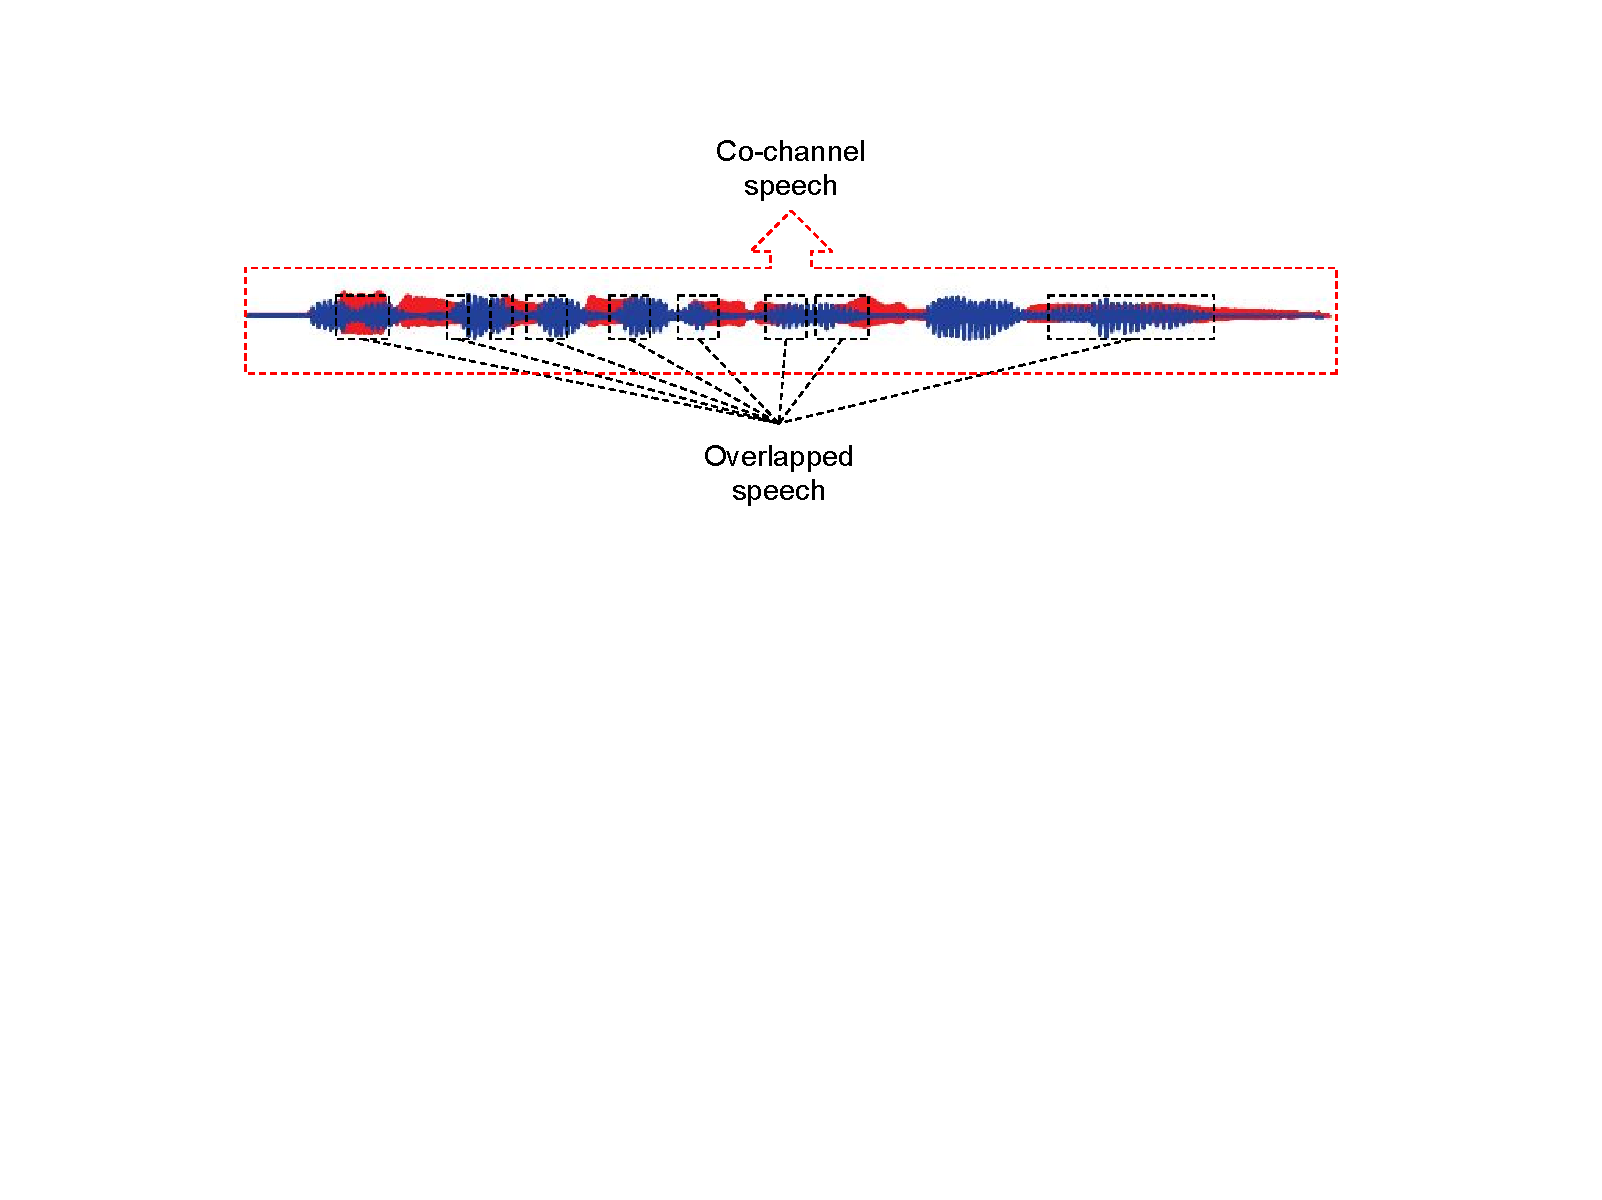
\includegraphics[height = 2in, width=0.9\textwidth]{figures/cochannel_vs_overlap-crop}
	\vspace{-3mm}
	\caption{\it \small Difference between co-channel and overlapped speech. Overlap refers to instances where more than one speaker is active. Co-channel is defined as an entire stream that contains multiple speakers. All co-channel files do not necessarily contain overlap. }
	\label{fig:cochannel_vs_overlap}
	\vspace{-3mm}
\end{figure}


%The specifics of recording conditions are overlooked in this study. 
%For example, information that relates to each speaker’s distance from the microphone and room acoustics. 
%This is intentional, since most of the difficulty in dealing with co-channel speech arises 
%from it being single-channel, which implies limited access to spatial 
%information as well as other sources of meta-data.

Aside from overlapped vs. non-overlapped speech, there are different ways of categorizing co-channel data in terms of how it is generated. 
Among such is a semantic classification that focuses on speakers' interactions with each other and divides co-channel data into two subgroups: 
\begin{itemize}
	\item conversational co-channel speech
	\item co-channel speech with independent parties
\end{itemize} 

Conversational co-channel speech refers to recordings in which speakers acknowledge other parties in the recording and engage in dialog. 
Alterations of speech production are an important artifact of conversational co-channel speech, which are the result of conscious and unconscious reactions of the foreground speaker and interferer(s). 
Examples of such alterations are raised pitch and energy level ~\cite{Shriberg01observationson,schegloff2000overlapping}. 
Raised Pitch and volume are especially common at or around overlaps. 
Readers are probably familiar with political debates with heated arguments. 
Most debates are perfect instances of an exaggerated version of the above-mentioned changes in speech production. 
Schegloff argues that long and sustained overlaps are primarily a sign of argumentative speech~\cite{schegloff2000overlapping}. 
In such conversations, most speakers tend to alter their voice in order to control the floor. 
These changes are problematic in automatic speech applications and are considered a type of distortion. 
Treatments are directed towards applications that suffer the most from speech alterations, predominantly automatic transcription of speech, i.e., speech recognition. 
Aside from changes in speech production, the element of interference by competing speakers is also an important artifact observed during overlaps. 
Therefore, in conversational co-channel data, one has to consider both overlaps and speaker specific alterations as sources of distortion and mismatch. 

Co-channel data with independent parties, are examples of co-channel data where the speakers do not interact with each other. 
An example of this types is cross-talk between separate channels; imagine switching between radio stations on an analog AM radio. 
The main characteristic of such data is that speakers are not aware of each other and therefore do not pertain to normal conversational mannerisms. 
That includes following turn-taking rules, which in most cases limits overlapped speech. 
Artificially generated co-channel data (mixing independent channels) is another example of co-channel speech with independent parties. 
A considerable portion of this study will focus on this type of co-channel data to analyze performance of overlap detection and also speaker recognition. 
We rely on this type of data since it provides the flexibility of controlling the amount of overlapped speech. 
As we will show in the next chapter, conversational co-channel speech does not necessarily contain sufficient overlapped data for some of our experiments. 
Therefore, we allow ourselves to neglect some aspects of conversational co-channel speech for the benefit of more overlap. 
That is why we value ``co-channel data with independent parties'', despite some of its unrealistic characteristics compared to conversational speech. 

The treatment of different speech processing applications for co-channel speech will focus on one of the two categories described above. 
This study will focus on a number of speech applications including: 
\begin{itemize}
	\item Signal processing and audio classification: identifying and separating overlapped segments in co-channel files. 
	\item Speaker recognition/verification: The ability to automatically decide whether two or more speech samples belong to the same speaker. 
	\item Speaker diarization: Segmenting an audio stream by counting the number of speakers as well as determining who spoke when. 
\end{itemize}

A description of an outreach to signal processing in vehicles is also presented, where algorithms developed for co-channel speech analysis were used to improve driver safety. 

\section{Approach}

The goal of this thesis is to provide tangible solutions to problems caused by co-channel speech in automatic speech technology. 
We argue that part of these issues are caused by overlapped speech (direct speech interference), which plays a significant role in making co-channel speech a difficult problem. 
The presence of overlapped speech can be detrimental to speaker diarization and speech recognition systems. 
%There is no clear and unique way of labeling or transcribing overlapped segments. 
In speaker diarization, it becomes difficult to assess system performance at overlaps, due to the inherent ambiguity in labeling overlapped segments. 
The same goes for speech recognition where aside from determining which is the ``primary'' speaker, recognizing speech at overlaps is more difficult, due to interference coming from other speakers. 
For this and other reasons detailed in the next chapter, the first portion of this study is devoted to overlapped speech detection. 
Our approach to overlap detection will be to focus on developing signal processing techniques to detect and separate overlap from single-speaker speech. Figure~\ref{fig:overlap_applications} depicts some applications of overlap detection in speech technology. 

\begin{figure}[h!]
	\centering
	\vspace{0mm}
	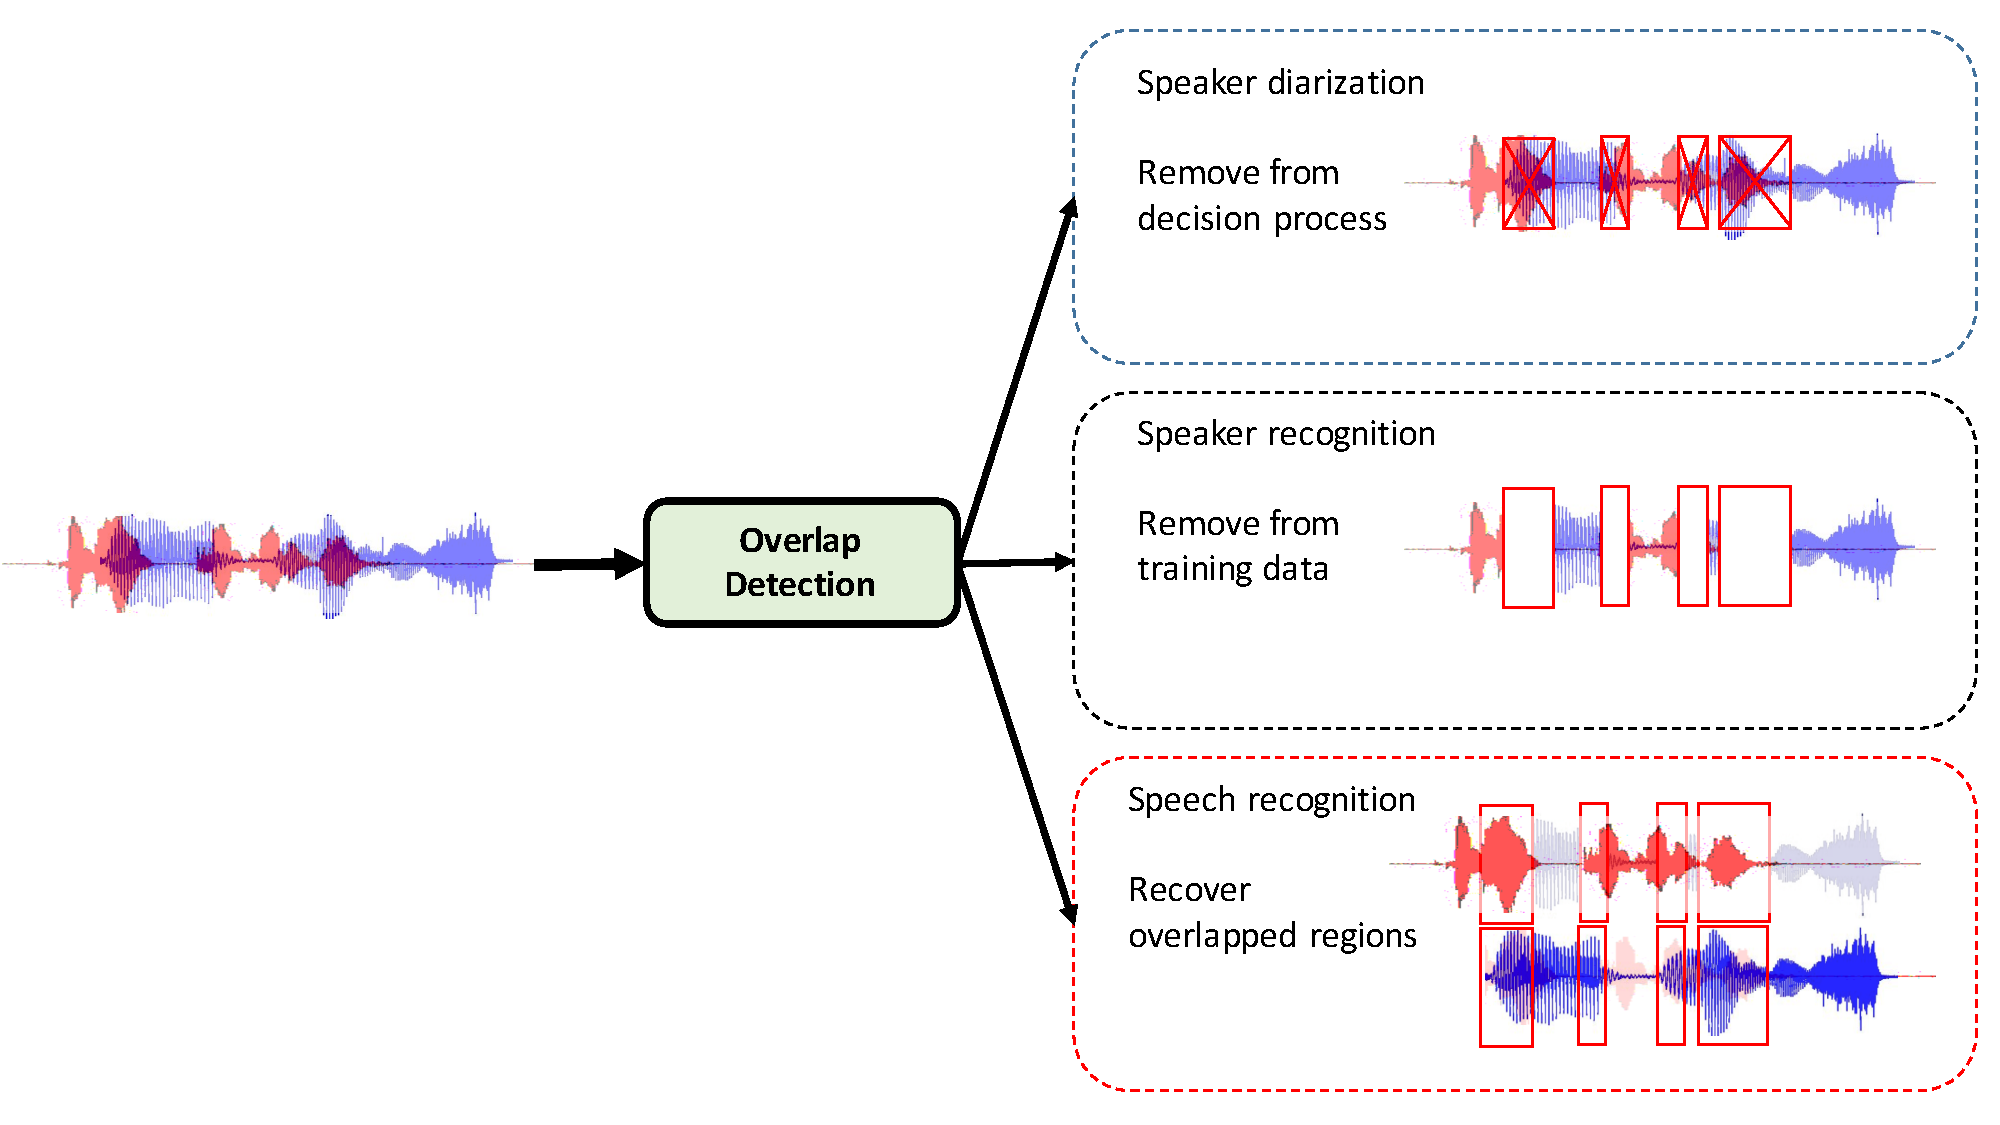
\includegraphics[height = 3in, width=\textwidth]{figures/overlap_detection_applications}
	\vspace{-3mm}
	\caption{\it \small Various applications of overlap detection. Top: In speaker diarization, ignoring overlapped regions provides a more fair assessment of diarization performance. Middle: Removing overlaps in speaker recognition increases the reliability of training data. Bottom: Overlap detection results can be used as an initial step to recover overlapped regions.}
	\label{fig:overlap_applications}
	\vspace{-3mm}
\end{figure}

Although overlap is considered an important aspect of co-channel speech, in many conversational speech data, the amount of overlap can be considered negligible, depending on the application. 
One such application is speaker recognition, which is also the main theme of this thesis. 
In text-independent speaker recognition, speech content (i.e., what is being said) is of less values compared to long-term speaker dependent characteristics (i.e., who is speaking). 
The standard approach in dealing with co-channel speech in such cases is speaker diarization. 
The role of diarization is to segment audio streams into shorter intervals each of which contains only one speaker. 
We consider speaker diarization a ``signal level'' approach. 
The term signal level is in respect to co-channel speech, since it is removed from the original signal prior to any other processing.
Alternately, a novel approach is presented in this study with the intention of bypassing the use of speaker diarization in the aforementioned scenario while preserving speaker recognition performance. 
This approach is to remove unwanted speaker-dependent information from latent variable subspaces generated from audio files~\cite{dehak2011front,kenny2010bayesian}. 
We refer to such solutions as ``subspace level''. 
Therefore, chapters III and IV each propose a different approach to remove interfering speakers from co-channel data. 
\begin{enumerate}
\item Remove interfering speakers in the feature subspace level: i-vector subspace factorization (Chapter III).
\item Remove interfering speakers in the signal level: speaker diarization (Chapter IV).
\end{enumerate}

Speaker diarization, will attempt to recognize and group speech that belongs to the same speaker in a co-channel audio stream. 
While subspace factorization maps speaker-dependent models to a subspace that will only contain parameters identifying the speaker of interest (aka primary speaker). 
Once again it should be pointed out that the main theme of this study is to address speaker recognition and identification in co-channel speech. 
Which makes speaker diarization an inseparable part of our approach. 





\chapter{FRONT-END SIGNAL PROCESSING}

\section{Introduction}
\label{sec:intro}
 
Overlapped speech constitutes a significant amount of research in co-channel speech. 
To such an extant that in many cases the terms co-channel and overlapped speech are used interchangeably. 
This chapter focuses on proposing signal processing techniques to recognize instances of co-channel data where speakers overlap; overlapped speech detection. 
Single-channel recordings from meetings or conversations are examples during which speakers may overlap. 
In fact, as shown in the previous chapter, the is a direct relation between the number of speakers and the possibility of overlap. 

Most studies on overlapped speech have focused on separating the target or suppressing interfering speech~\cite{morgan_cochannel}. 
Often to de-noise and thereby improve the performance of automatic speech applications~\cite{Quat_Dan_cch_sup,Chazan_93,cooke20101} (primarily speech recognition). 
However, over the past decade, due to increased interest in recognition systems such as speaker identification (SID) and diarization, a growing trend of detecting overlapped regions has been observed. 
In speaker identification, the presence of interfering speech in conversational speech styles not only reduces the effectiveness of trained speaker models but also increases the uncertainty in scoring test files with overlapped regions~\cite{yantorno_report}. 
Removing overlapped segments increases model reliabilities which consequently improves recognition~\cite{shokouhi2015}.    
State-of-the-art speaker diarization systems are also currently at a stage where one of the main sources of error is the presence of overlapped speech~\cite{boakye_icassp_08,zelenak12Trans}. 
One of the main reasons overlaps become a source of confusion in speaker diarization systems is that there is no basis for selecting ground-truth in overlapped regions. 
This makes evaluating speaker diarization systems more challenging\footnote{Future chapters will describe co-channel speech data in speaker diarization in more detail.}. 
Fortunately, for applications such as speaker identification and diarization it is rarely necessary to separate the target from interfering speaker in overlapped speech, since preserving speech content is not a priority. 
One can improve system performance by detecting and excluding overlapped segments for both SID and diarization. 
In other, removing a corrupt (in this case overlapped) speech segment usually does more good then harm in such applications. 
Replacing interferer suppression and target separation with overlapped speech detection, is sometimes called ``usable speech detection''\footnote{In order to avoid any confusion between this study and the assumptions made in \cite{yantorno_report}, we use the more general term overlapped speech detection.} \cite{yantorno_report}. 
An overlapped speech detection system can be used in any of the aforementioned tasks as a data purification step or a signal processing front-end. 

\begin{figure*}[t!]
	\centering
	\vspace{0mm}
	%\textbf{Overlap Detection Applications}\par\medskip    
	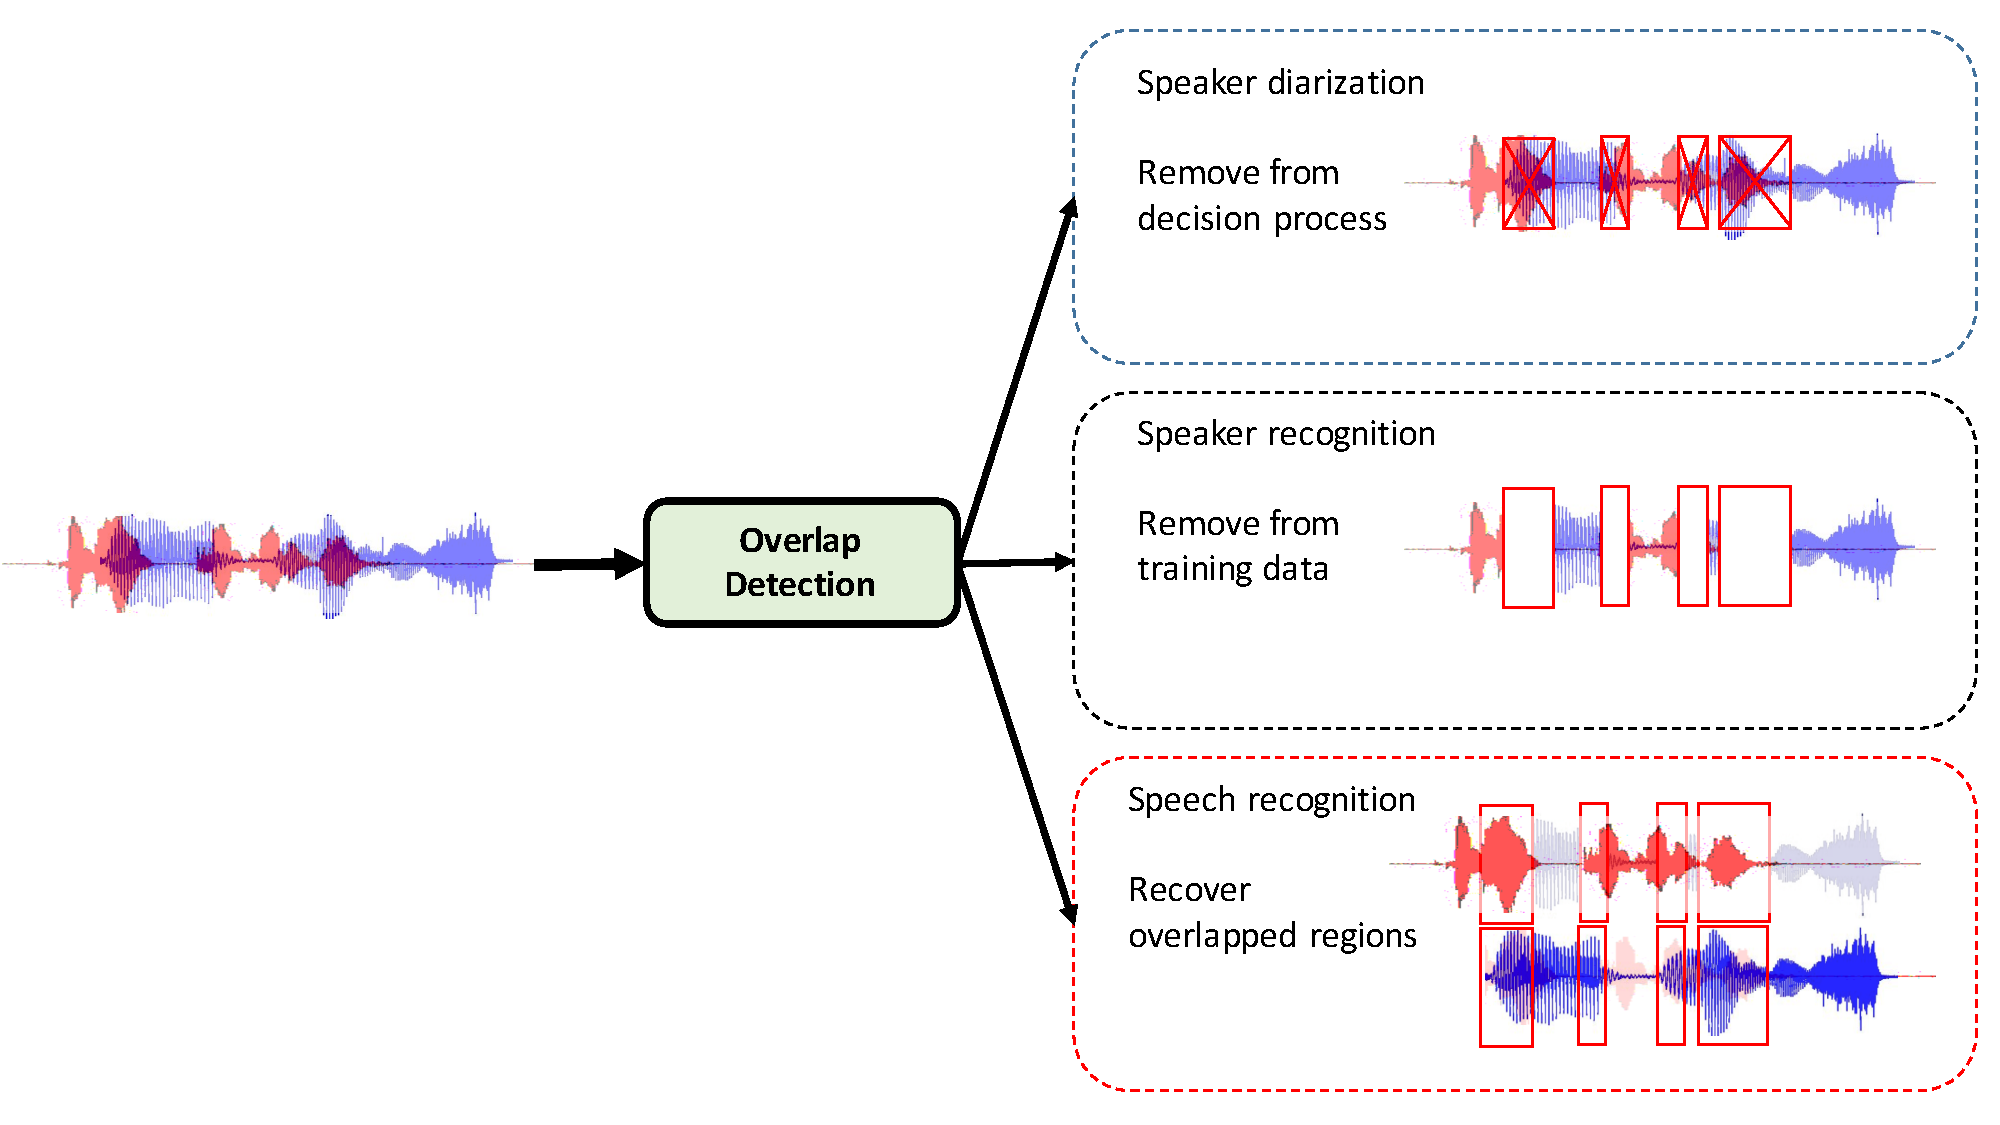
\includegraphics[height = 3in, width=0.9\textwidth]{figures/overlap_detection_applications}
	\vspace{-3mm}
	\caption{Applications of overlap detection. 
	Top: In speaker diarization, removing ignoring overlapped regions provides a more fair assessment of diarization performance. 
	Middle: Removing overlaps from in speaker recognition increases the reliability of training data.
	Bottom: Overlap detection results can be used as an initial step to recover overlapped regions.}
	\label{fig:pykno_blockdiag}
	\vspace{-3mm}
\end{figure*}

Signal processing front-end solutions in our study focus solely on overlapped speech detection. 
Figure~\ref{fig:pykno_blockdiag} summarizes incorporating overlap detection in speech processing technology. 


Detecting overlapped segments has previously been considered in tasks such as speaker identification (SID) and speaker diarization~\cite{boakye_thesis,yantorno_report}. 
In such problems, the presence of a secondary speaker either decreases model reliability (in training), or introduces confusion in the decision-making process by distorting test files. 
Detecting overlaps is computationally advantageous to enhancing the desired speaker's speech when one has the luxury of neglecting overlapped data~\cite{yantorno_report}. 
As is the case for speaker recognition and diarization~\cite{Boakye_is_08}. 
By detecting overlapped speech, we are able to remove them from the training and decision-making process. 
We begin this chapter by demonstrating the effects of manipulating the amount of overlapped data in speaker verification experiments. 
This will give us an understanding of how much overlaps affect speaker identification. 
In addition, we will see how introducing overlaps to speaker verification affects train and test data separately. 


\section{Overlaps in Speaker Verification}
\label{SID_in_GRID}

In this section, in order to show the detrimental effects of adding overlapped data to speaker verification, we present a case study of speaker recognition on data from the monaural speech separation challenge~\cite{cooke20101}. 
Our experiments use $12$-dimensional MFCC features ($13$ excluding the $0^{th}$ coefficient) plus $\Delta$ and $\Delta\Delta$, which adds to a total of 36 dimensional features. 
The experiments use the Gaussian mixture model (GMM) approach where a trained speaker is model using a mixture of Gaussians and the maximum likelihood of a given test audio file is computed from the train model. 
GMM parameters are obtained through maximum a-posterior adaptation of the parameters of a speaker independent GMM (called a universal background model which is trained on a large pool of speakers). 
We only MAP adapt GMM means in our experiments. 
$512$ mixtures were used to form the Universal background model (UBM). 
This setup requires a model for the train speakers (for whom we have several recording sessions available), but for the test speakers we only use the features to compute the ML probability of the test features belonging to the corresponding train speaker in each trial. 
The figure below summarizes the speaker verification setup. 

\begin{figure*}[h!]
	\centering
	\vspace{0mm}
	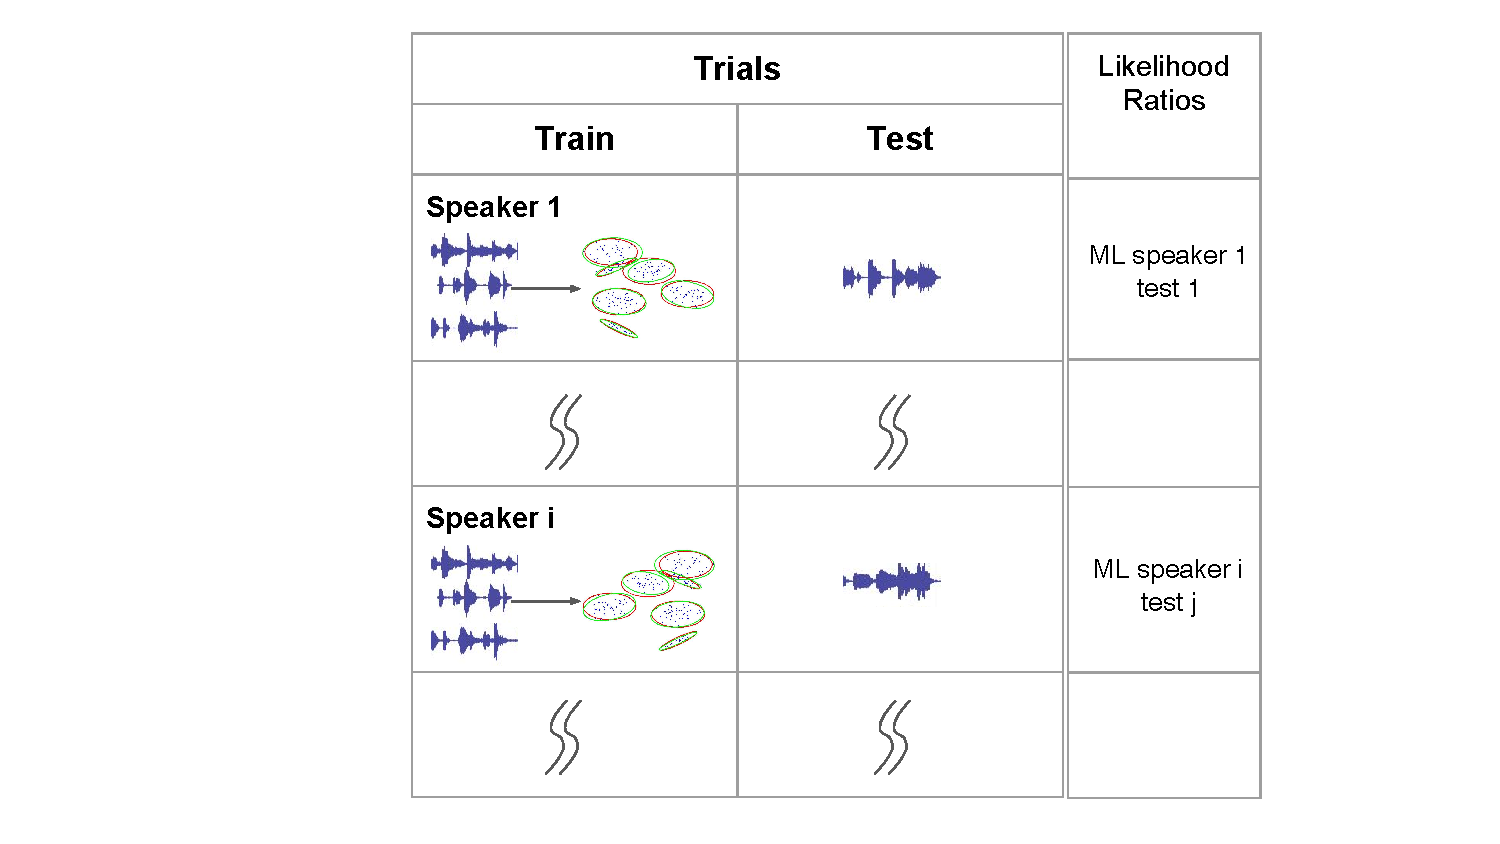
\includegraphics[height = 3in, width=0.5\textwidth]{figures/speaker_verification_setup}
	\vspace{-3mm}
	\caption{GMM-UBM speaker verification setup.}
	\label{fig:gmm_ubm_verification}
	\vspace{-3mm}
\end{figure*}


\subsection{Overlaps in test data}
As a comparison benchmark, we first evaluate SID performance under clean train and test conditions on the SSC data.
Gaussian mixture models (GMM) are adapted from a Universal back model (UBM) trained on TIMIT files~\cite{msridentity}.
For each model speaker, there are 500 utterances in SSC, which are all used in the training process. Test files are available in all SIR conditions.
As expected, lower SIR values correspond to higher equal error rates.
The presence of a secondary speaker, clearly causes confusion in the score distribution, leading to less separability between target and imposter trials.
SID performance under clean test files and those with average SIR ranging in $+6, +3, 0, -3
, -6, -9 dB$ are provided in Fig.~\ref{fig:sidingrid_ovlintest_train_a}.

It is worth mentioning that the authors were tempted to compare these results with stationa
ry noise experiments.
However, contrary to our expectations, we observed that performances were better in the ove
rlapped condition when compared to white Gaussian noise and speech-shaped noise interferenc
e, even for negative SIR values.
We find this to be a misunderstanding caused by comparing stationary and non-stationary noi
se through the same measurement procedure, which is the SIR (or SNR).
For a given target speech file, adding a certain amount of stationary noise will affect all frames, whereas in the case of non-stationary noise (here speech) only a portion of the frames receive non-uniform interference.
This leads to incomparable results under presumably similar conditions which we decided to exclude from this study to avoid confusion.

%\begin{figure*}[t!]
%	\centering
%	\begin{subfigure}[t]{0.5\textwidth}
%		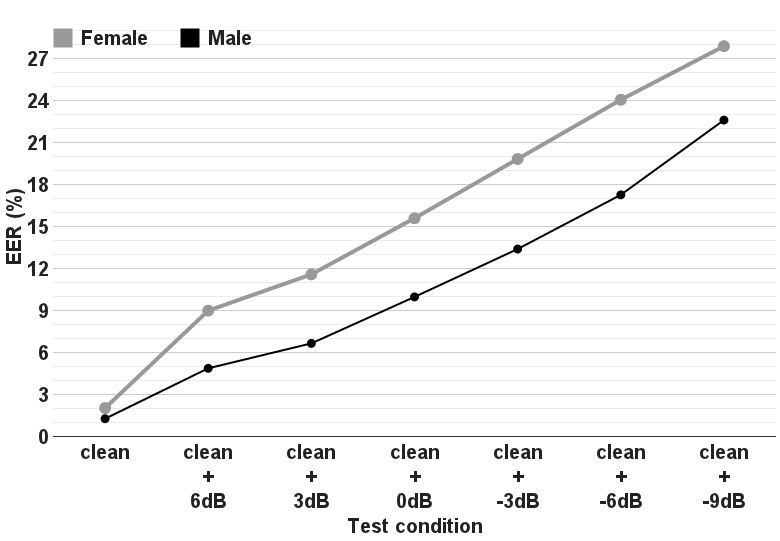
\includegraphics[width=\textwidth]{figures/sidingrid_ovlintest}
%		\vspace{-1mm}
%		\caption{~}
%		\label{fig:sidingrid_ovlintest_train_a}
%	\end{subfigure}%
%	~ %add desired spacing between images, e. g. ~, \quad, \qquad, \hfill etc.
%	%(or a blank line to force the subfigure onto a new line)
%	\begin{subfigure}[t]{0.5\textwidth}
%		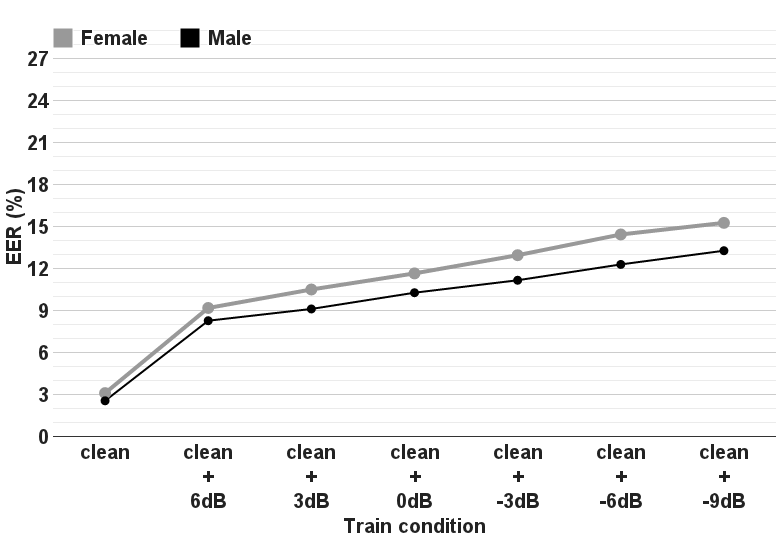
\includegraphics[width=\textwidth]{figures/sidingrid_ovlintrain}
%		\vspace{-1mm}
%		\caption{~}        \label{fig:sidingrid_ovlintest_train_b}    \end{subfigure}    \vspace{-3.6mm}
%	\caption{The rise in EER values as we increase the effect of overlapped speech (via decreasing the SIR). Starting from clean (i.e. single-speaker speech) to lower SIR values. a) Shows the case where train files are clean, but test files contain overlaps.  b) clean test files but train files contain overlaps.}
%	\vspace{-1.2mm}
%\end{figure*}
%
%\begin{figure}[!t]
%	\vspace{2mm}
%	%\centering
%	\begin{subfigure}[b]{0.3\textwidth}
%		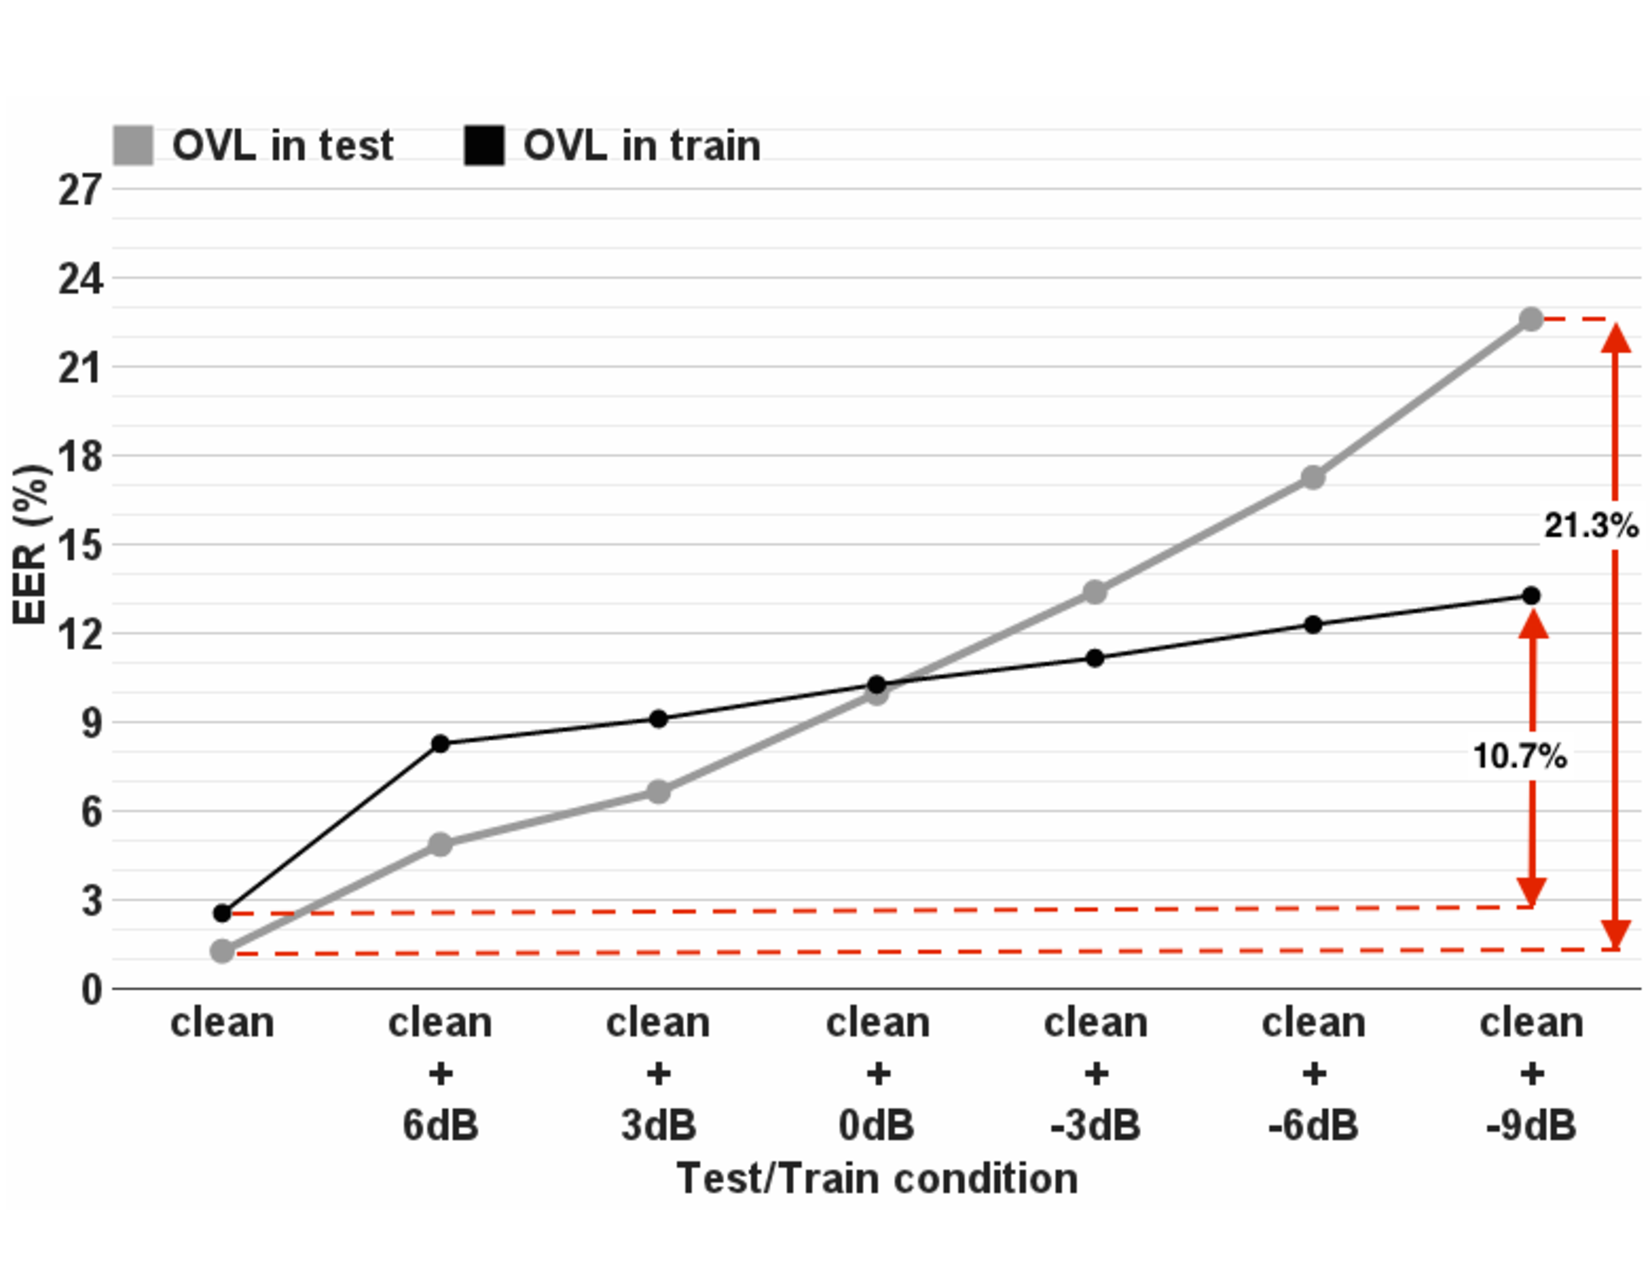
\includegraphics[height = 2.43in, width=1.6\textwidth]{figures/sidingrid_ovlintrainvstest_male_rev1}
%		\caption{male}
%		\label{fig:sidingrid_ovlintrainvstest_male}
%	\end{subfigure}
%	\begin{subfigure}[b]{0.3\textwidth}
%		\hspace{0.7\textwidth}
%		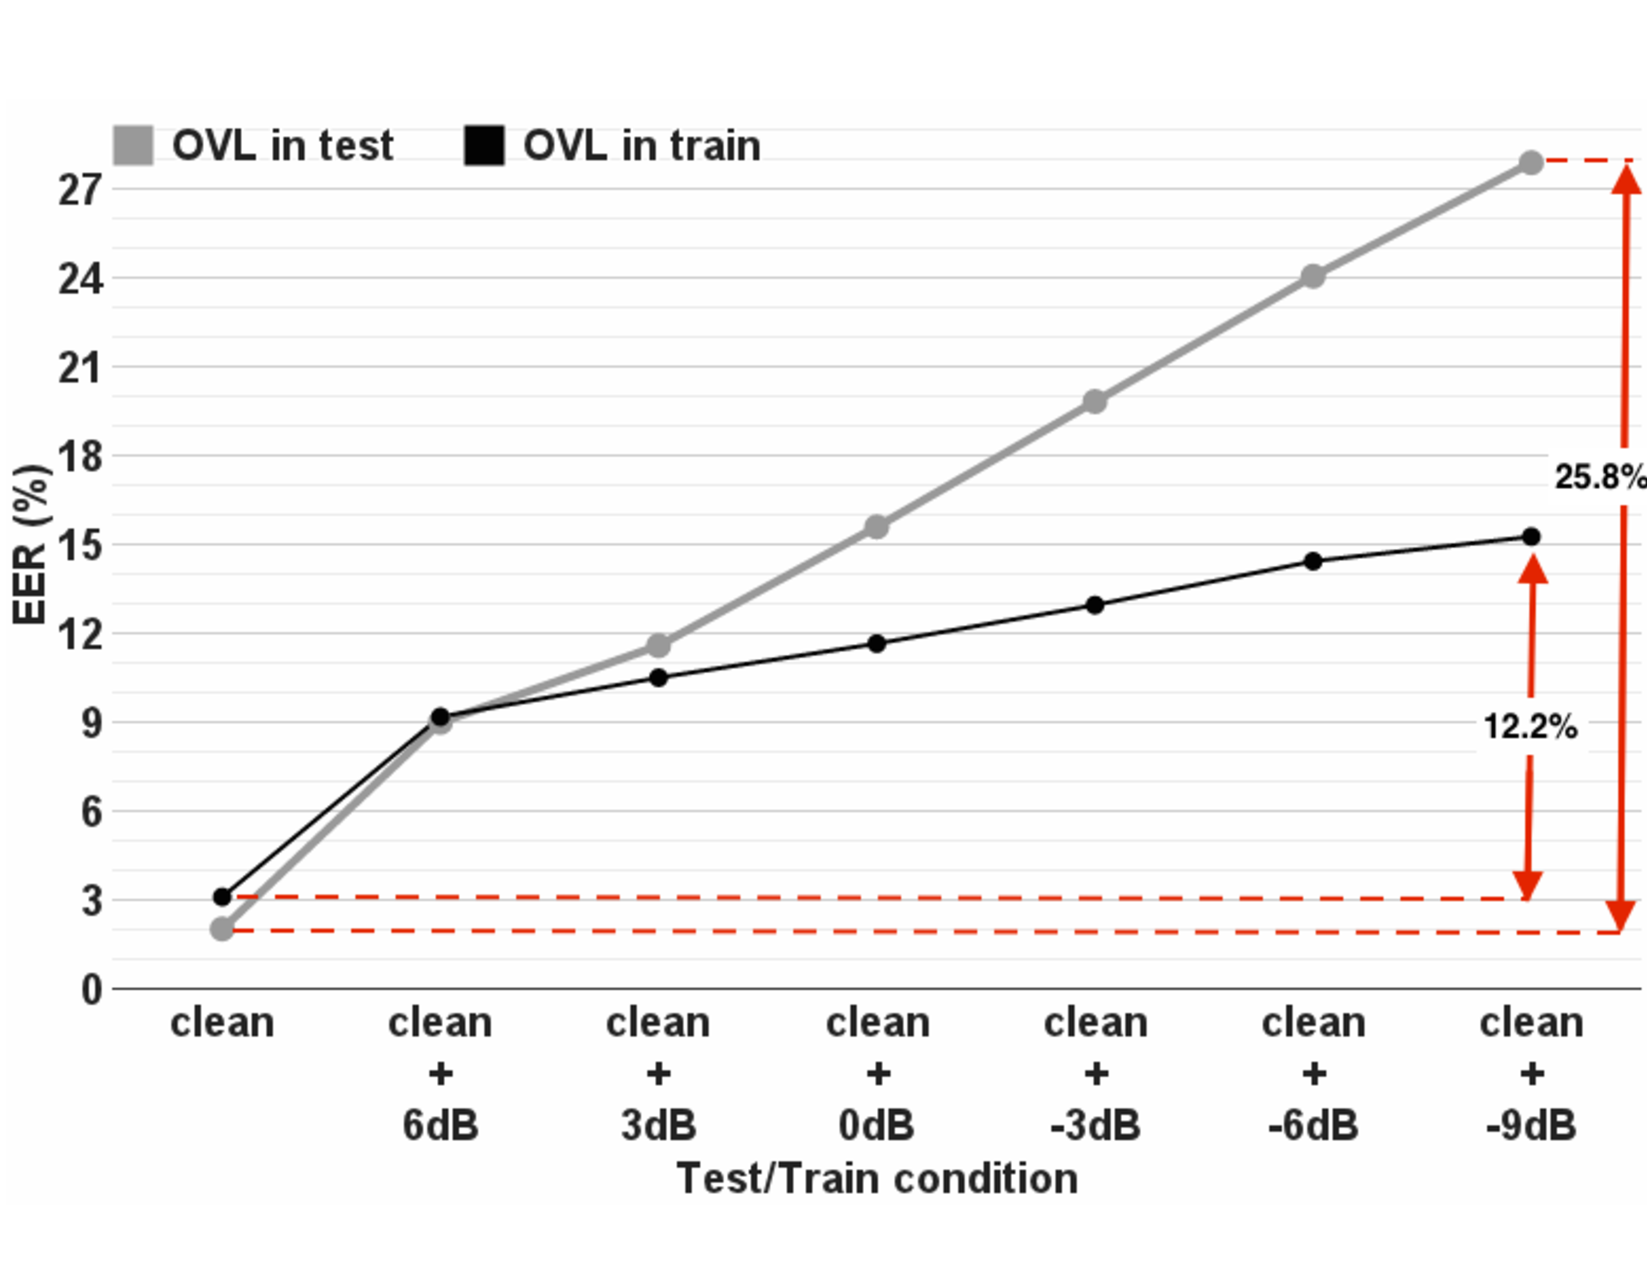
\includegraphics[height = 2.43in, width=1.6\textwidth]{figures/sidingrid_ovlintrainvstest_female_rev1}
%		\caption{female}
%		\label{fig:sidingrid_ovlintrainvstest_female}
%	\end{subfigure}
%	\caption{Comparing the impact of increasing overlap (OVL) in train vs. test data by decreasing SIR values. Experiments for male (a) and female (b) speakers. Lower SIR drops the performance more rapidly when applied to test data.}
%	
%	\vspace{2mm}
%\end{figure}

\subsection{Overlaps in train data}
We also examine the effect of adding overlapped speech to train files.
Figures~\ref{fig:sidingrid_ovlintrainvstest_male} and \ref{fig:sidingrid_ovlintrainvstest_female} compares the effects of adding overlapped speech in train and test files.

An interesting observation is the higher rate with which the EER increases when the SIR drops for the test condition.
We believe this is due to the fact that in train conditions, the training of Gaussian mixture models tends to cancel out the effect of the interfering speech.
For each speaker, the GMM is trained on a set of features, some of which are influenced by the desired speaker and the rest influenced by the interfering speakers.
Since multiple training files are used to model each speaker (different training files have different interfering speakers), the GMM tends to converge to a common locale in the feature space, which belongs to the speaker for whom the models are being trained.
We call this effect averaging out (or cancelling out) of the interfering speakers.
This to some extent slows the growth in EER as the data becomes noisier in train files.
Such cancellation, however, does not exist across test files.

\section{Background}

Traditionally, studies have used spectral harmonicity as a key factor in detecting overlapped speech~\cite{nav_icassp13,smolenski_tut}. 
This approach is motivated by the fact that two fundamental frequencies exist in most instances of overlapped speech which disarranges the harmonic structure observed in single-speaker speech. 
As a side-note here, we point out that most focus in overlapped speech has been at regions where both speakers produce ``voiced'' speech. In~\cite{morgan_cochannel} a classification of different types of segments in co-channel speech is presented. Figure~\ref{fig:morgan_v_uv_table} is adopted from~\cite{morgan_cochannel}. 

\begin{figure}[h!]
	\centering
	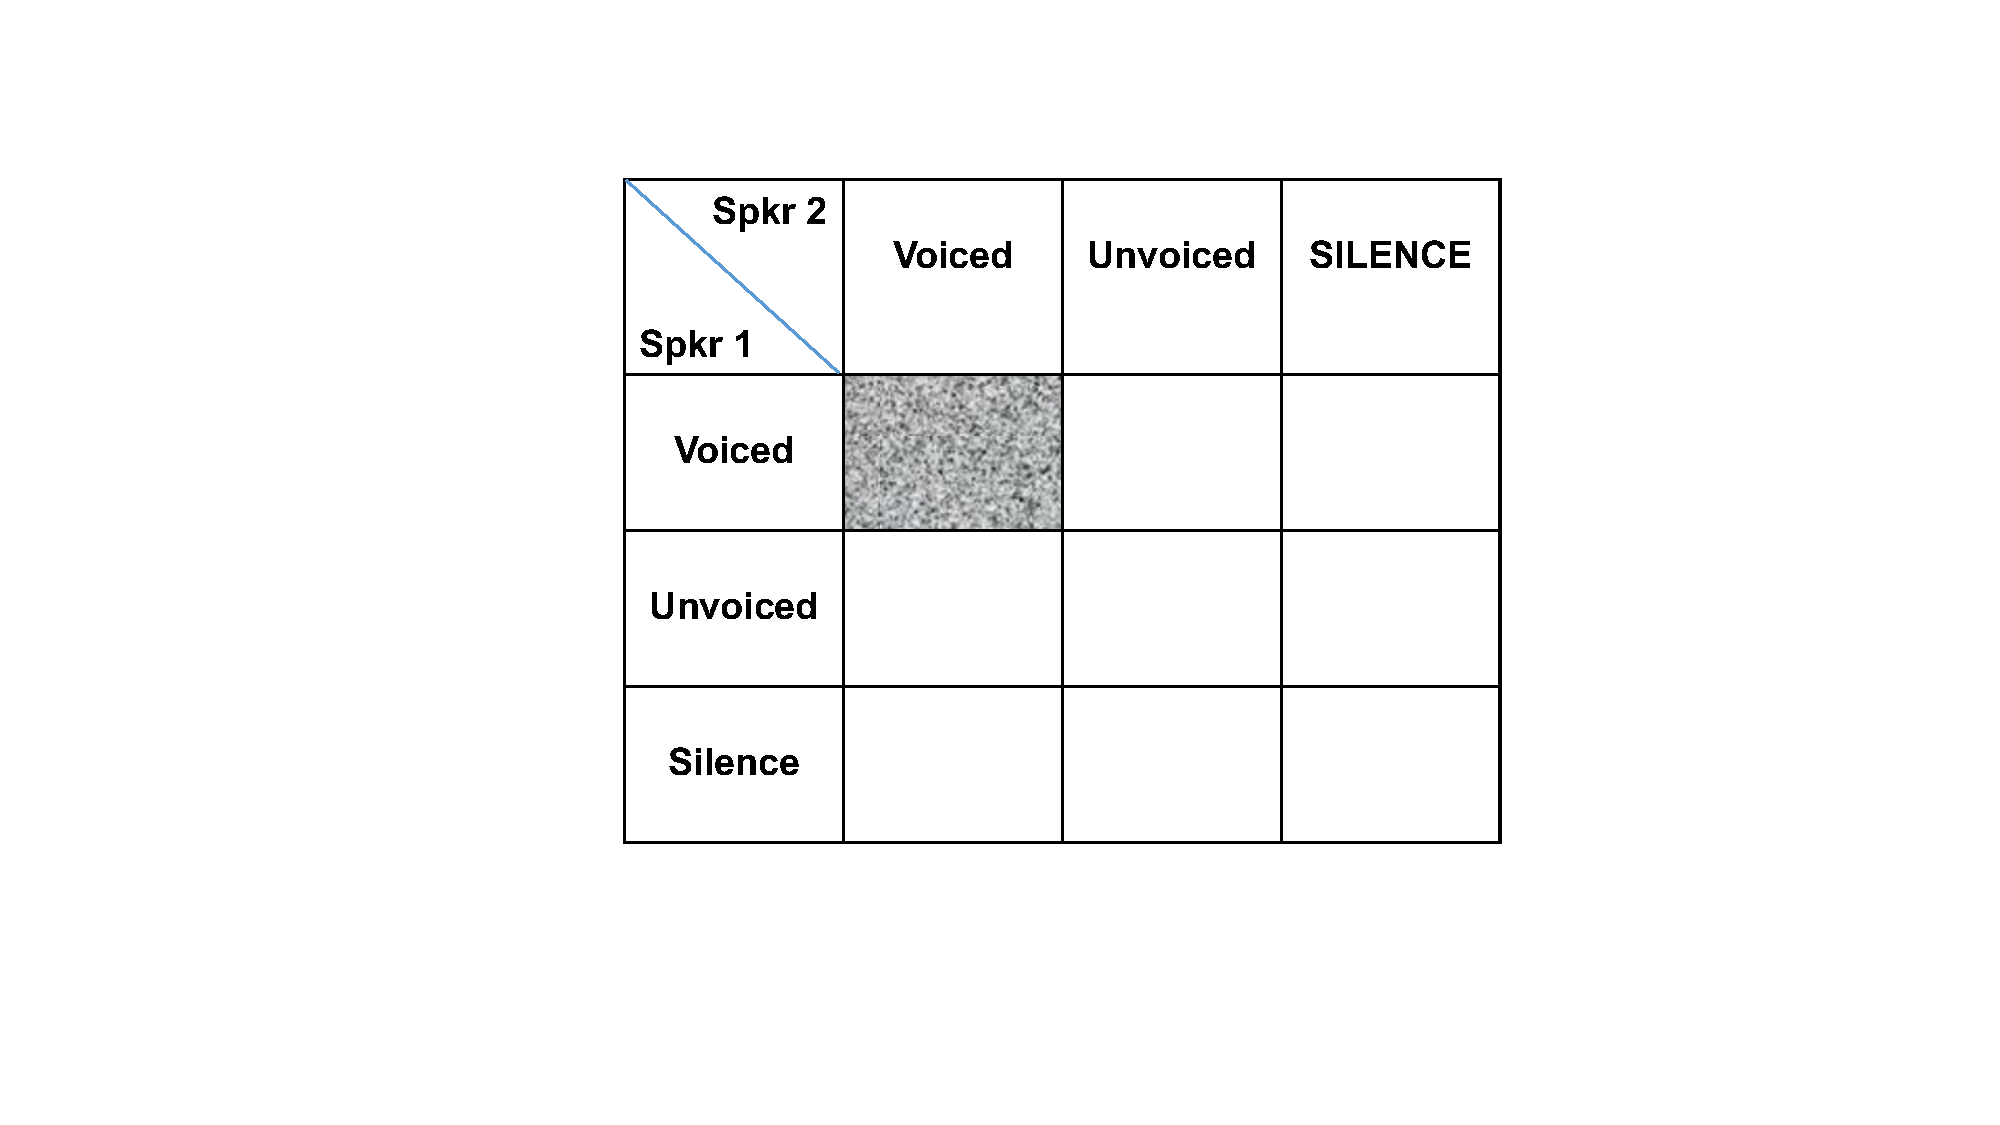
\includegraphics[height = 3.1in, width=0.5\textwidth]{figures/morgan_v_uv_table}
	\label{fig:morgan_v_uv_table}
	\caption{Classification of different segments in a co-channel file. In overlap detection we are interected in 
		the voiced-voiced (shaded) region.}
\end{figure}

Most of our focus will be on the voiced-voiced cell. 
Merely because detecting other regions becomes far more difficult. 
A more detailed classification of overlapped regions is presented in~\cite{fig:nav_icassp13}, where a grid containing all phones is used to rank-order overlapped segments in terms of difficulty. 
The analysis in~\cite{fig:nav_icasssp13} expands Fig.~\ref{fig:morgan_v_uv_table} as shown in Fig.~\ref{fig:nav_v_uv_table}. 
General consensus is to focus on detecting voiced-voiced overlap detection, which from now on we will refer to as overlap detection. 

\begin{figure}[h!]
	\centering
	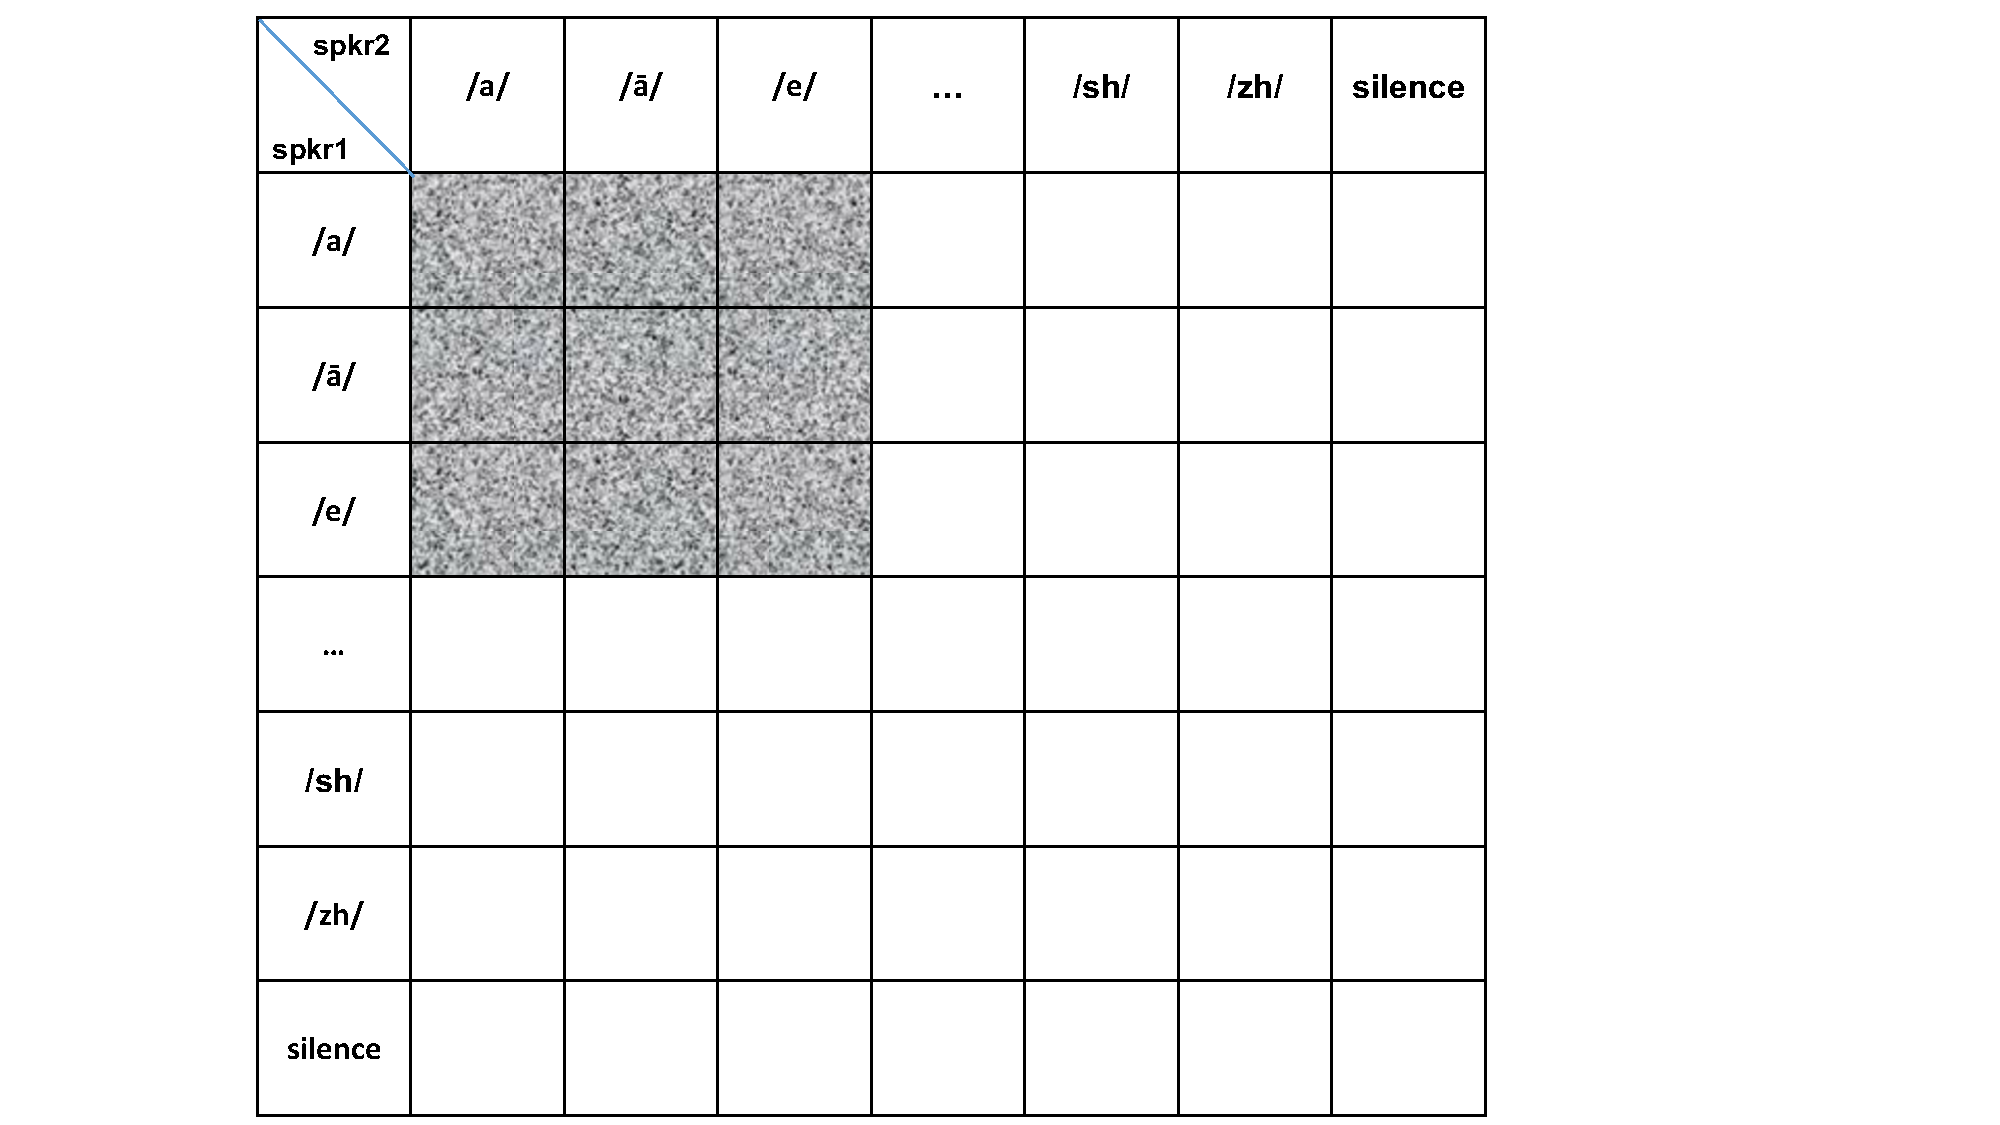
\includegraphics[height = 3.1in, width=0.5\textwidth]{figures/nav_v_uv_table}	
	\label{fig:nav_v_uv_table}
	\caption{phone-based expansion of overlapped segments in Fig.~\ref{fig:morgan_v_uv_table}.}
\end{figure}

Concentrating on voiced speech allows us to use more discriminating harmonic structures to detect overlaps. 
In~\cite{sapvr_2000}, the peak-to-valley ratios in frame-based spectral autocorrelations are introduced as a discriminating feature for overlapped speech detection through the same assumption. 
Spectral flatness measure, the ratio of geometric to arithmetic means calculated from spectral bins in a speech frame, has also been used as a measure to capture harmonicity and has been used to detect the presence of overlapped speech~\cite{nav_icassp13}. 
Another related characteristic is observed when monitoring fundamental frequencies along time. 
Adjacent pitch period comparison (APPC) presented in~\cite{appc2001} uses the temporal variation of estimated ``pitch'' periods as a measure to detect ``usable'' speech with the assumption that temporal variations of adjacent pitch periods are significantly higher in overlap. 
A multi-pitch tracking algorithm proposed in~\cite{Dwang_03_trans} was used in~\cite{Dwang_03} to estimate coexisting fundamental frequencies in the presence of multiple speakers. 
Regions where more than one fundamental frequency is estimated are labeled as overlap. 
The multi-pitch tracking technique described in~\cite{Dwang_03_trans}, decomposes speech into sub-bands and pitch estimation is only performed on reliable sub-bands. 

A slightly different, yet fundamentally similar, approach to distinguish overlapped speech is to use speech kurtosis which measures higher order moments of the signal statistics~\cite{Wrigley_05}. 


A number of studies have considered investigating spectral characteristics at formant frequency locations when dealing with overlapped speech. 
Giuliani et al. use a filter-based approach to improve speech recognition rates for different instances of meeting conditions by adding a detection step that separates double-speaker speech from single-speaker audio~\cite{giuliani_meeting}. 
This was accomplished by cascading two-layer sub-band filters to capture formant characteristics. 
Formant frequency information was obtained by filtering the signal at sub-bands with center frequencies and bandwidths corresponding to nominal ${F_1, F_2}$, and ${F_3}$ values for all English vowels. 
One of the reasons Formant-based overlapped speech analysis has received less attention is the difficulties in modeling pole interactions at overlapped regions, which is an issue for linear predictive modeling and other commonly used formant tracking techniques. 
Characterizing pole interactions using standard LP models easily becomes intractable in the presence of more than one source. 
Add to this complication, the unknown speaker locations with respect to each other and the microphone. 
As a result, we focus our attention to nonlinear speech models, some of what have proven more successful in the scenarios described above. 

Nonlinear speech models, including the AM-FM speech model~\cite{maragos_kaiser_quatieri} have been used in previous studies to model speech resonances without any specific requirements for the source signal. 
These energy operators have also been used to deal with signals with more than one source~\cite{maragos_instantaneousenergy}, aka co-channels signals~\footnote{Co-channel is a more general terminology used to described multi-component signals. 
In the case of speech, co-channel speech may refer to any single-channel recording that contains speech from multiple speakers, regardless of whether there is overlap.}. 
Maragos et al. use higher order energy operators to develop an algorithm that simultaneously demodulates the components of a co-channel mixture in AM-FM modulated signals~\cite{maragos_instantaneousenergy}. 
Litvina et al. separate speech from music using the Teager energy operator (TEO) separation algorithm~\cite{maragos_kaiser_quatieri}~\cite{Litvin2010}, where they used the extracted components to design a time-varying filter and suppress the interfering signal. 
Similar multicomponent signal decomposition techniques have been addressed using energy operators to separate narrow-band signals~\cite{Linicassp95,hu12_nullspacepersuit,santhanam_maragos_2000}. 

Our goal is to incorporate sub-band analysis to design a technique suitable for {\bf overlapped speech detection}. 
Two algorithms are proposed that incorporate sub-band analysis for overlap detection. 
\begin{itemize}
	\item using TEO methods on narrow-band components to detect speech harmonics. 
	\item apply cosine functions across sub-band outputs to magnify the presence of multiple harmonics. 
\end{itemize}


%%%%%%%%%%%%%%%%%%%%%%%%%%%%%%%%%%%%%%%%%%%%%%%%%%%%%%%%%%%%%%%%%%%%%
%%%%%%%%%%%%%%%%%%%%%%%%%%%%%%%%%%%%%%%%%%%%%%%%%%%%%%%%%%%%%%%%%%%%%
%%%%%%%%%%%%%%%%%%%%%%%%%%%%%%%%%%%%%%%%%%%%%%%%%%%%%%%%%%%%%%%%%%%%%
%%%%%%%%%%%%%%%%%%%%%%%%%%%%%%%%%%%%%%%%%%%%%%%%%%%%%%%%%%%%%%%%%%%%%

\section{Pyknograms}
\label{sec:ovldet}

We propose a novel approach for overlapped speech detection based on an enhanced spectrogram. 
These spectrograms, called Pyknograms, were first introduced by Potamianos and Maragos in~\cite{potamianos_maragos_icassp95,potamianos_maragos_jasa96} and are calculated by applying multi-band demodulation in the AM-FM speech model framework~\cite{maragos_kaiser_quatieri}{\footnote{The authors in~\cite{potamianos_maragos_jasa96} used the term ``Pyknogram'' which stems from the Greek word ``pykno'' meaning dense. Pyknograms represent highly resonating regions in time-frequency plots as populated scatter plots, hence the term density.}. 
Pyknograms provide a more prominent representation of harmonic trajectories, which we propose to use as a means to detect the presence of interfering speech.


\subsection{Energy Operators and the AM-FM speech model}

In Pyknograms~\cite{potamianos_maragos_jasa96}, the harmonic structure of speech is enhanced by decomposing spectral sub-bands into amplitude and frequency components. 
This multi-band analysis uses the AM-FM speech model~\cite{maragos_kaiser_quatieri} to decompose sub-bands and thereby calculate corresponding instantaneous frequencies and bandwidths: (\ref{eq:instamp}),~(\ref{eq:instfreq}). 
Pyknogram extraction locates dominant peaks in the spectrogram from instantaneous frequencies. 
To extract Pyknograms, the speech signal is initially passed through a filter-bank (we have modified the algorithm to use logarithmically spaced Gamma-tone filters, while~\cite{potamianos_maragos_jasa96} uses linearly-spaced Gabor filters). 
Filter-bank outputs are then decomposed into amplitude and frequency components using the discrete energy separation algorithm (DESA-1)~\cite{maragos_kaiser_quatieri}, where the frequency and amplitude components of a given sub-band, $x(n)$, are calculated using the discrete energy operator,
 

\begin{equation}
\Psi [x(n)] = x^2(n)-x(n-1)x(n+1),
\end{equation}
$\Psi [x(n)]$ is energy operator used to estimate amplitudes and instantaneous frequencies, as shown in Fig.~\ref{fig:desa1}. 


\begin{equation}
\label{eq:instfreq}
f(n) = \frac{1}{2\pi}\arccos \Big (1-\frac{\Psi[x(n)-x(n-1)]}{2\Psi[x(n)]}\Big),
\end{equation}
 
 
\begin{equation}
\label{eq:instamp}
|a(n)| = \sqrt{\frac{\Psi[x(n)]}{\sin^2(2\pi f(n))}}.
\end{equation}



\begin{figure}[b]{3.5in}
	\centering
	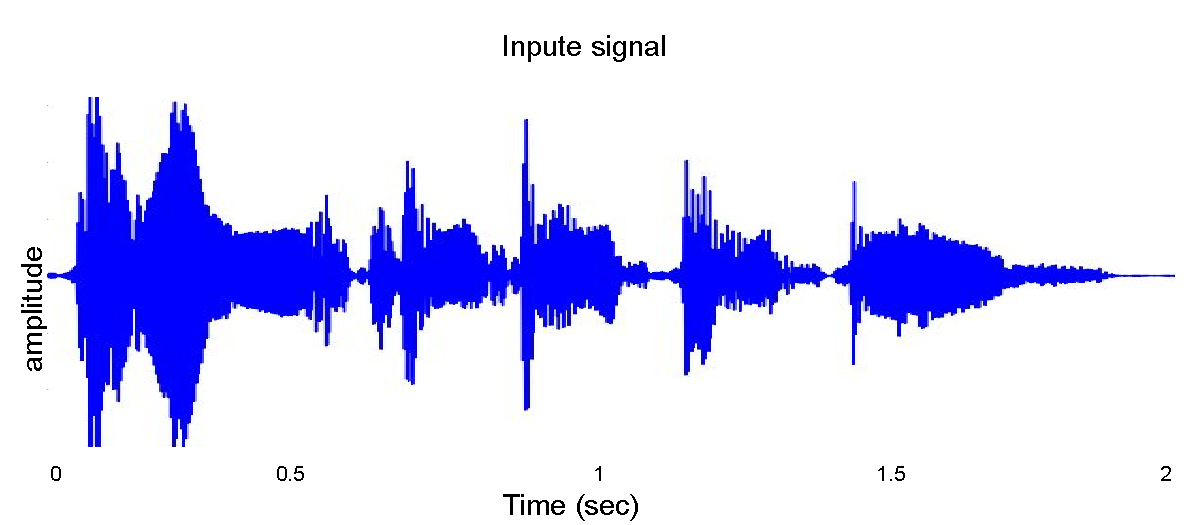
\includegraphics[height=1.5in, width=4in]{figures/teo_signal}
	\caption{Input signal.}
\end{figure}
	
\vspace{1.0mm}
\begin{figure}[b]{3.5in}
	\centering
	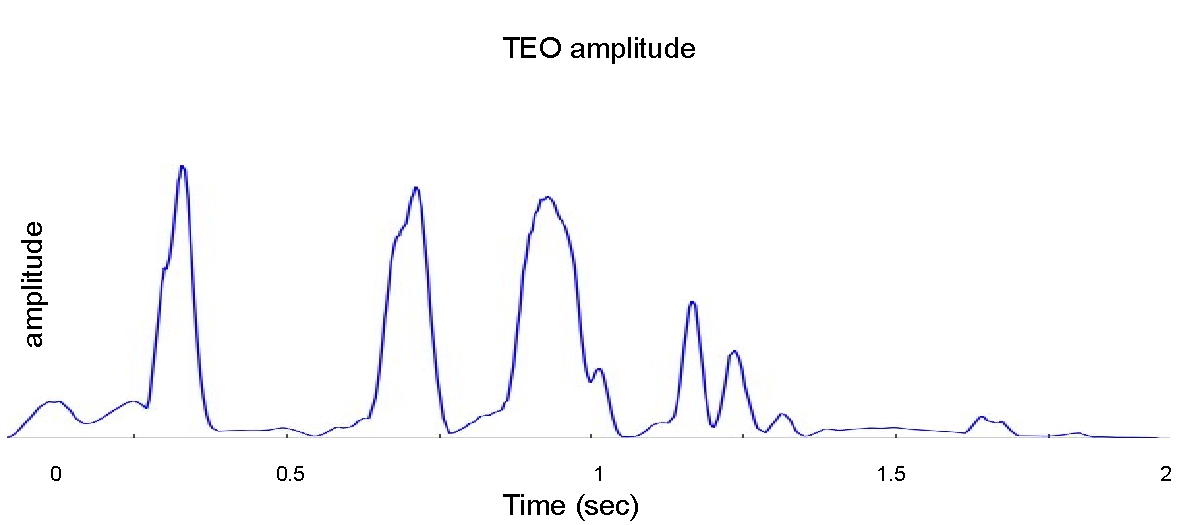
\includegraphics[height=1.5in, width=4in]{figures/teo_amp}
	\caption{Outputs of DESA-1: Signal amplitude component estimated using TEO, Eq.~(\ref{eq:instamp}).}
\end{figure}

\begin{figure}[b]{3.5in}
	\centering
	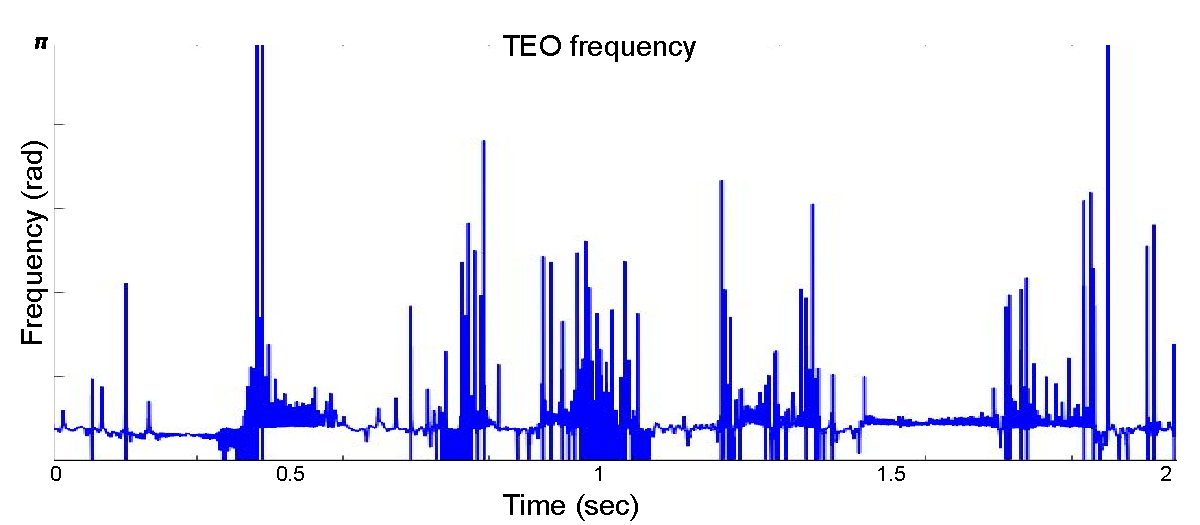
\includegraphics[height=1.5in, width=4in]{figures/teo_freq}
	\caption{Outputs of DESA-1: Signal frequency component estimated using TEO,  Eq.~(\ref{eq:instfreq}).}
\end{figure}

\subsection{Pyknogram Extraction}
\label{ssec:pyknogram_extraction}

Pyknograms are estimated from DESA-1 outputs. The weighted average of instantaneous frequency components (see~(\ref{eq:weighted_f})) is used to derive a short-time estimate of the dominant frequency in each sub-band over time-frame units (typically 25 msec)~\cite{cohenlee90}. 
Frequencies are weighted using the estimated signal power ($|a(n)|^2$). 
The average frequency computed for each frame/sub-band (time-frequency unit) can be viewed as the $1^{st}$-order moment of instantaneous frequencies.  


\begin{equation}
\label{eq:weighted_f}
F_w(t) = \frac{\sum_{t}^{t+T}f(n)a^2(n)}{\sum_{t}^{t+T}a^2(n)},
\end{equation}
The algorithm also provides a means to estimate weighted bandwidths for each resonance, (\ref{eq:weighted_bw}). 
What we refer to here as bandwidths are essentially $2^{nd}$-order frequency moments. 

\begin{equation}
\label{eq:weighted_bw}
B_w(t) = \sqrt{\frac{\sum_{t}^{t+T}(\overset{\boldsymbol .}{a}(n) /2\pi)^2+(f(n)-F_w)^2a^2(n)}{\sum_{t}^{t+T}a^2(n)}},
\end{equation}
where $f(n)$ and $a(n)$ are instantaneous frequency and amplitude values from (\ref{eq:instfreq}) and (\ref{eq:instamp}). 
In (\ref{eq:weighted_f}), the instantaneous frequencies are averaged over the $t^{th}$ frame using squared instantaneous amplitudes as weights. 
$T$ in (\ref{eq:instfreq}) is the number of samples per frame, from $n = t$ to $n = t+T$. 
$\overset{\boldsymbol .}{a}(n)$ is the first difference of $a(n)$ (i.e., $a(n) - a(n-1)$). 
The per-frame values of $F_w$ provide initial estimates of spectrogram peaks. 
This results in a time-frequency {$t$-$f$} representation of the overall signal, where time units correspond to frames and frequency units to filter-bank sub-band indexes. 


In~\cite{potamianos_maragos_jasa96}, the bandwidth values defined in (\ref{eq:weighted_bw}) are used for analysis purposes. 
Here, we use them in overlap detection systems to determine the reliabilitiy of $t-f$ units. 
Our assumption is that large Pyknogram bandwidths correspond to higher uncertainty in frequency estimates. 
We investigate this in following sections by adding an uncertainty term to our frequency estimate proportional to the estimated bandwidth:



\begin{equation}
\label{eq:jitter_f}
\tilde F_w(t) = F_w(t) + \epsilon_t,
\end{equation}
where
\begin{equation}
\label{eq:jitter_pdf}
\epsilon_t \sim\ \mathcal{N}(0,B_w(t)).
\end{equation}

As a final step, dominant harmonic peaks are selected by comparing the average frequency estimates with filter-bank center frequencies. 
According to~\cite{potamianos_maragos_jasa96}, points at which filter-bank center frequencies coincide with the weighted frequency estimates from (\ref{eq:weighted_f}) are more reliable in estimating spectrogram peaks. 
The assumption being that frequency estimates are more accurate when aligned with a filter in the filter-bank. 
This defines the condition through which initial $F_w$ values are tested to detect whether they correspond to prominent peaks. At frame $t$: 
\vspace{0mm}
\begin{equation}
\label{eq:RF1}
F_w(c) = c  \quad \iff \quad \{c \in peaks\}
\vspace{1mm}
\end{equation}
where $c$ are the filter-bank center frequencies. 
Note that center frequencies are distributed in a logarithmic scale. 
Another peak selection condition (as shown in Fig.~\ref{fig:pykno_blockdiag}) is to limit the relative variance of selected frequencies with respect to center frequencies. 

\begin{equation}
\label{eq:RF1}
\frac{\partial F_w(c)}{\partial c} < thr
\vspace{1mm}
\end{equation}
This condition limits non-harmonic anomalies that break the patterns in regular speech trajectories. 
Since such patterns are frequently observed in overlapped data, we omit this restriction from the peak-picking step.  

\begin{figure*}[t!]
	\centering
	\vspace{0mm}
	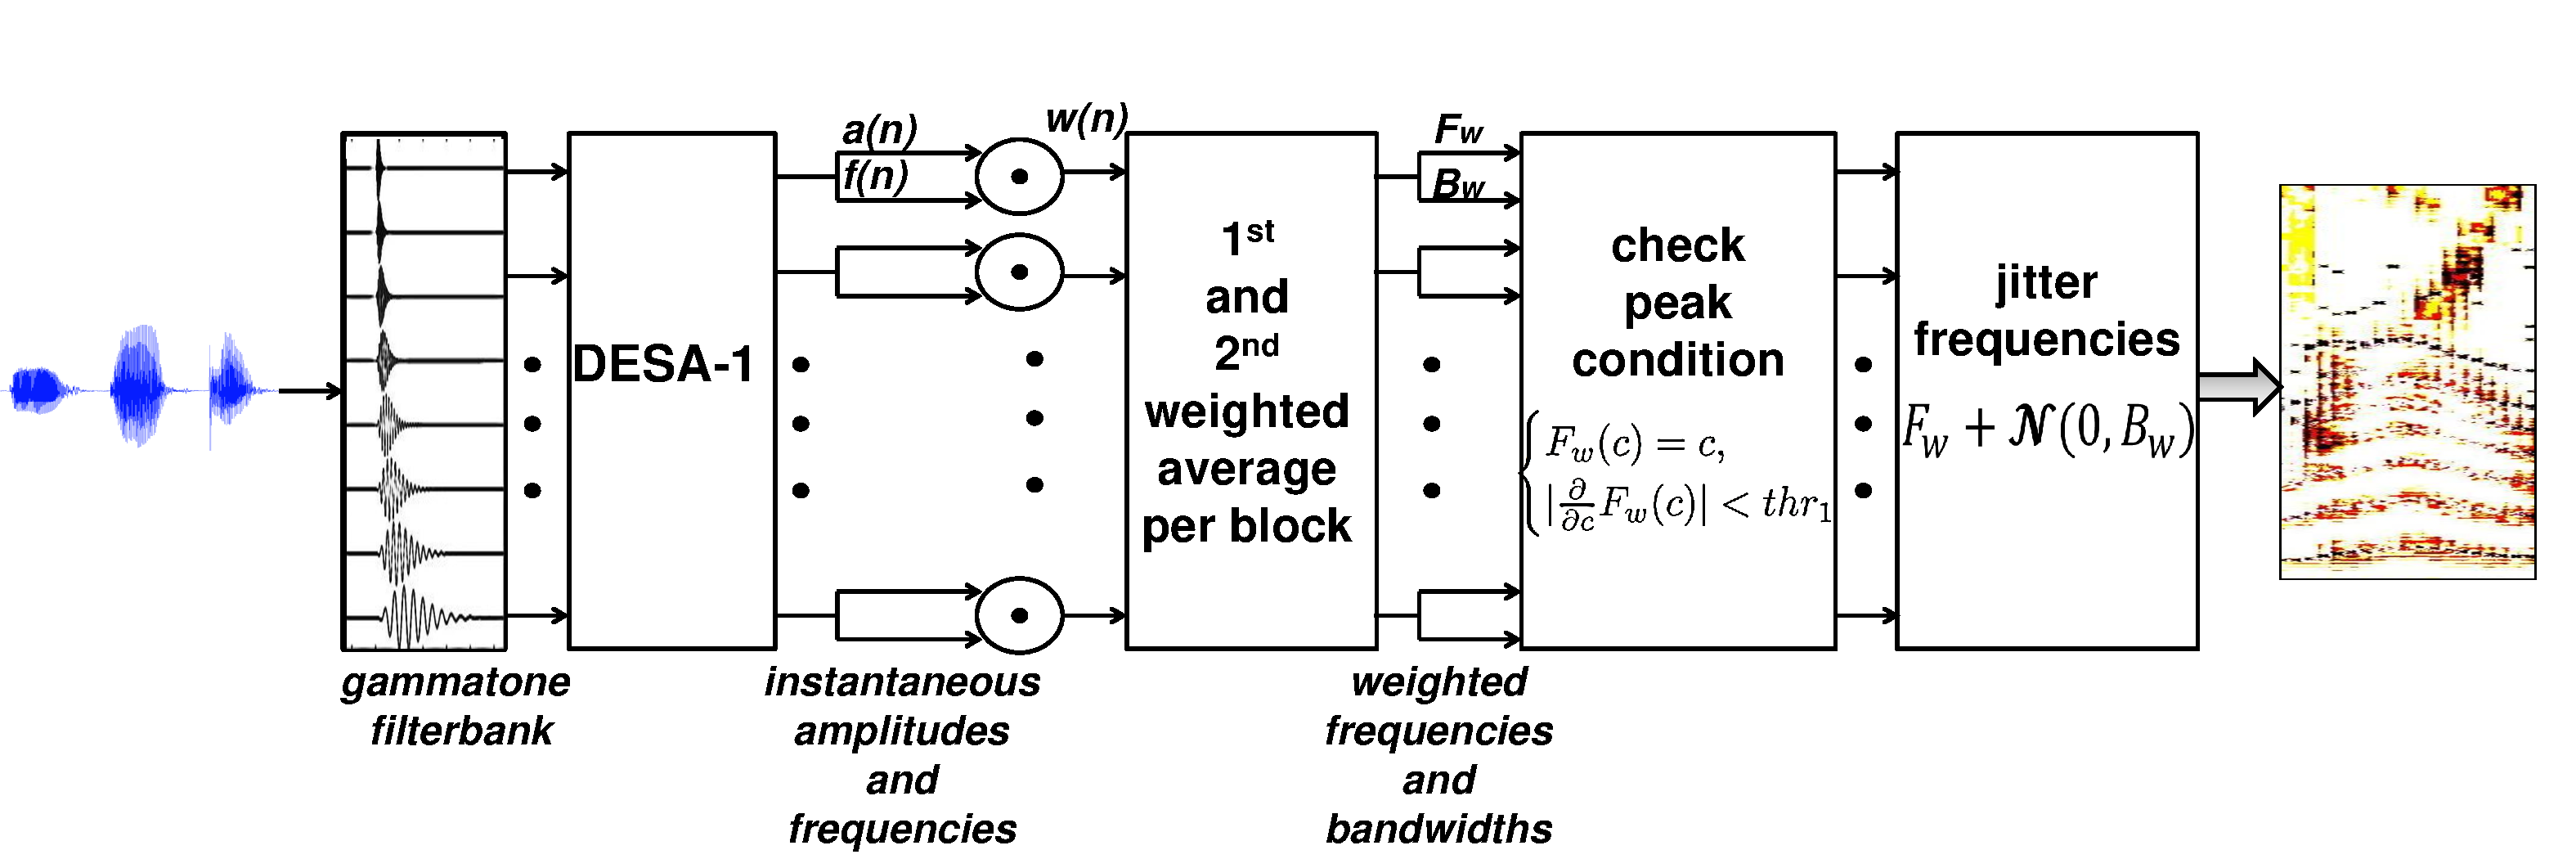
\includegraphics[height = 2.5in, width=1\textwidth]{figures/pyknogram_blockdiagram}
	\vspace{-3mm}
	\caption{Pyknogram extraction block-diagram.}
	\label{fig:pykno_blockdiag}
	\vspace{-3mm}
\end{figure*}


One of the advantages of the peak-picking constraint in (\ref{eq:RF1}) is the quantization of spectrograms onto filter-bank center frequencies. 
This allows the mapping of all signals onto a unified space defined by the filter-bank, which enables reliable comparison within the time-frequency space. 

Using an energy operator based approach helps avoid assumptions on the number of speakers in the signal. 
AM-FM decomposition is suitable since it relies on signal resonances and does not restrict signals to a specific structure or number of speakers (as opposed to models such as linear prediction). 
The final time-frequency representation is called a Pyknogram and is denoted $S_{pyk}(t,f)$ as a function of time ($t$) and frequency ($f$). 
Using Pyknograms, we would like to investigate overlap detection methods.

%\subsection{Detecting overlapped segments from Pyknograms}
Discontinuities in the Pyknogram layout is an indication of interfering speech. 
An analogy for speech harmonic patterns are skiing tracks left behind on a snowy surface. 
In the single-speaker case, the patterns leave parallel tracks that progress relatively slowly over time and correspond to fundamental frequency harmonic tracks. 
In the presence of an interfering speaker, these patterns are distorted by similar but intersecting tracks, which adds sudden jumps along the time axis (as shown in Fig.~\ref{fig:pyknograms_for_overlaps}). 
Since the majority of speakers are only capable of producing one fundamental frequency at each time instance, it is expected that the harmonic tracks should be consistent across time. 
This keeps harmonics parallel over short time intervals.   
The presence of a second speaker creates harmonic tracks that in general do not follow the same patterns, hence discontinuities are observed along time in Pyknograms. We use variations across adjacent frames as our measure of overlapped speech.

\begin{figure}[h!]
	\centering
	\vspace{4mm}
	\textbf{Pyknogram}\par\medskip
	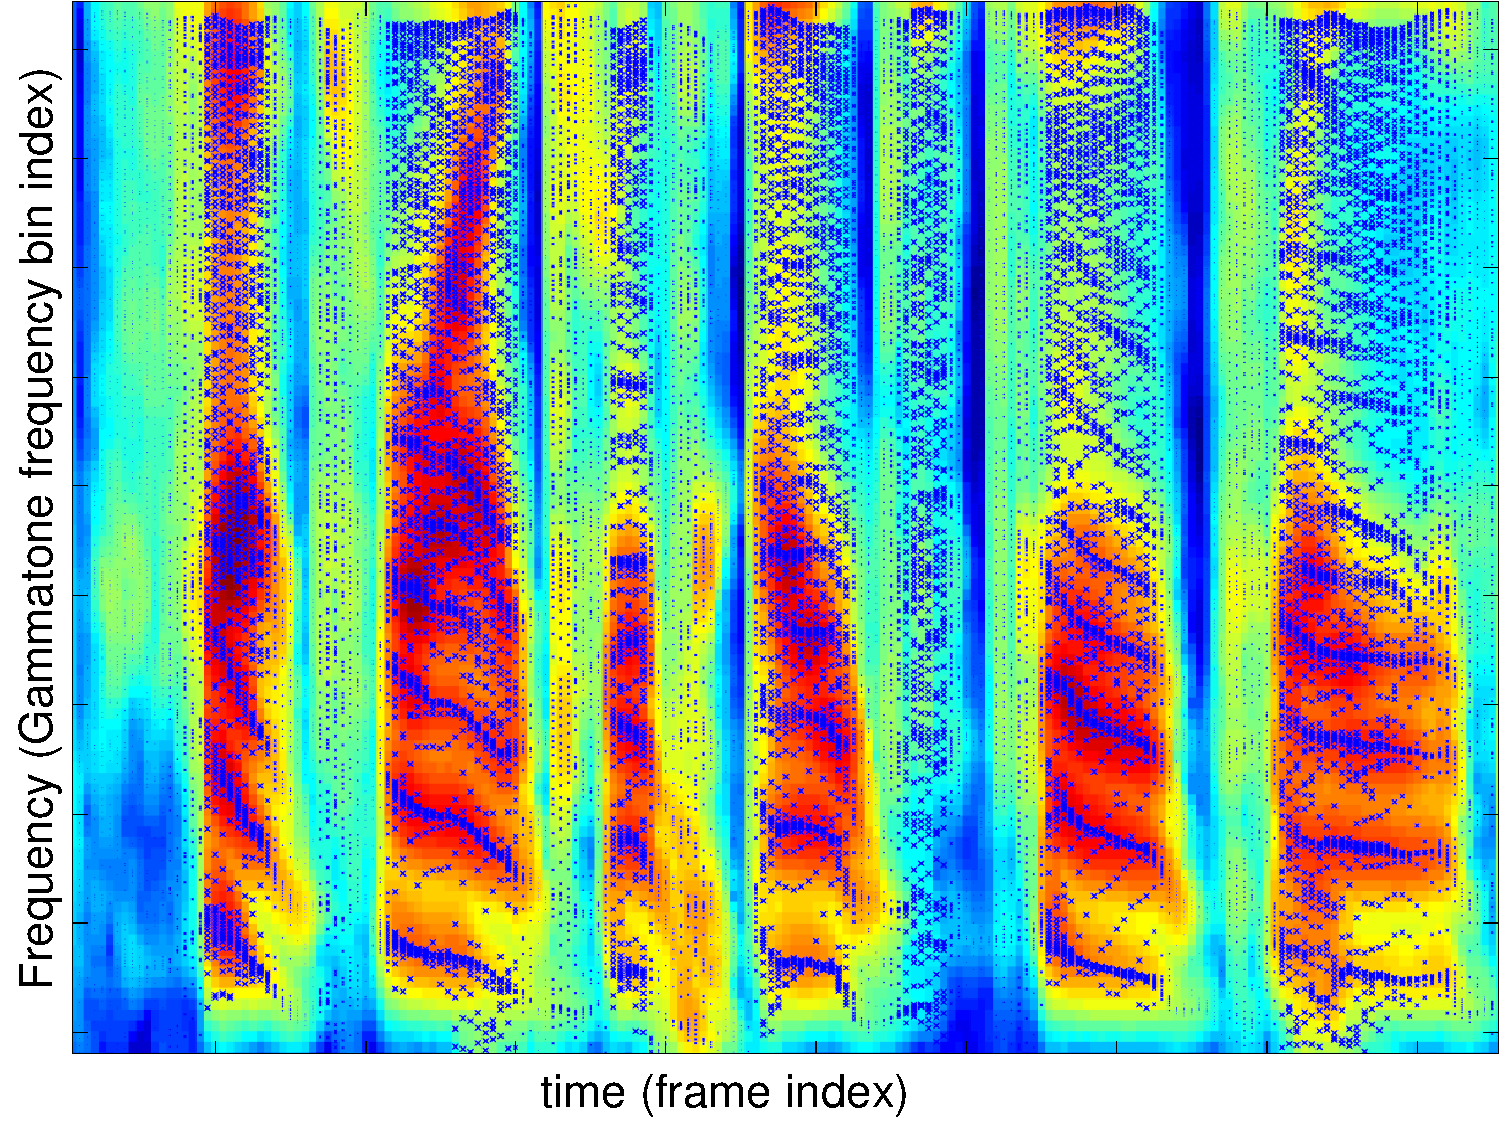
\includegraphics[height =3.in, width=0.8\textwidth]{figures/pyknogram_vs_spectrogram}
	\vspace{-1mm}
	\caption{Pyknogram for a given speech signal. The spectrogram is plotted in the background for comparison. Pyknogram markers have been scaled by the amplitudes of corresponding $t$-$f$ units. Frequencies are scaled to equivalent rectangular bandwidth (ERB) rate.}
	\vspace{-1mm}
	\label{fig:pyknograms}
\end{figure}

\subsection{Unsupervised overlap detection Pyknograms}

The average Euclidean distance between consecutive frames across all frequencies can be used to detect sudden jumps in Pyknograms along time. 
Similar to the technique used for spectral flux estimation~\cite{Rossignol_spectralflux}. 
The distance function, $D_{ovl}$, at frame $t$ is computed as the $2$-$norm$ distance between consecutive Pyknogram frames, $S_{pyk}(t,f)$ and $S_{pyk}(t-1,f)$. 

\begin{equation}
\label{eq:ovl_det_score}
D_{ovl}(t) = \sqrt{\sum_f\Big(\big(S_{pyk}(t,f)-S_{pyk}(t-1,f)\big)^2\Big)}
\end{equation}
where $t$ and $f$ respectively correspond to the frame index (time) and filterbank bin (frequency). 

Overlapped segments are expected to have higher $D_{ovl}$ values as compared to single-speaker speech. 
Figure~\ref{fig:pyknograms_for_overlaps} shows instances where sudden jumps are observed in the Pyknogram of an overlapped signal. 
The average value of these distances for all frames in a speech segment corresponds to the amount of overlapped regions (higher values are associated with greater overlap). 

\begin{figure}[h!]
\centering
\vspace{1mm}
    \textbf{Pyknogram close-up}\par\medskip
\vspace{-1mm}
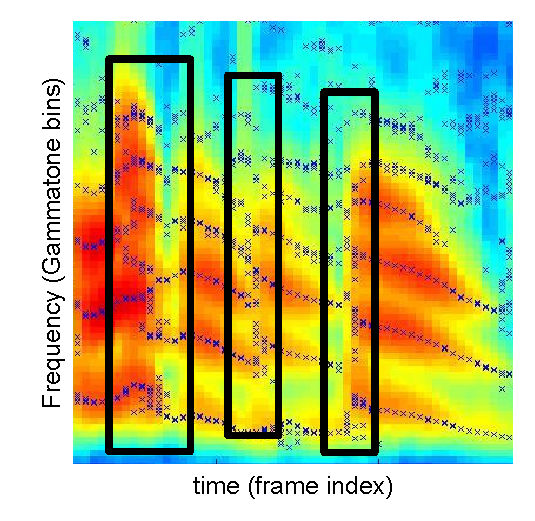
\includegraphics[height =2.0in, width=0.4\textwidth]{figures/co-channel_pyknogram-crop}
\vspace{-1mm}
\caption{A closer look on Pyknograms for overlapped speech. The enclosed patches show discontinuities that occur in the presence of an interfering speaker.}
\vspace{-1mm}
\label{fig:pyknograms_for_overlaps}
\end{figure}


We evaluate the performance of our proposed detection metric on overlapped speech from the GRID database~\cite{SSC_link}(see Sect.\ref{sec:exp} for more details on GRID). 
A key factor that determines the difficulty of detecting the presence of overlapped speech is the signal to interference(SIR) value. 
Greater absolute SIR values correspond to regions where one of the speakers has lower impact on the signal energy. 
Therefore it is more difficult to detect the occurrence of overlap in signals as the SIR moves away from $0dB$. 
Notice we use absolute SIR, since in overlap {\it detection} there is no difference between target and interfering speakers. 

Another important factor in detecting overlap is that the SIR value will change across different frames within a single file, which is due to the non-stationary nature of speech. 
This poses major restrictions on the effectiveness of overlap detection evaluation, since providing frame-based ground-truth becomes unrealistically difficult. 
One must therefore rely on ensemble measurements over complete speech files for which the average SIR is known. 
This notion is illustrated in Fig.~\ref{fig:compare_perframe_and_perfile_ovldethist}, where $D_{ovl}$ distributions (histograms) extracted on a per-frame basis are compared with ensemble $D_{ovl}$ distributions associated with each file. 
The ``scores'' ($D_{ovl}$ values) in Fig.~\ref{fig:compare_perframe_and_perfile_ovldethist} are pyknogram distances calculated using (\ref{eq:ovl_det_score}). 
The top figure (Fig.~\ref{fig:compare_perframe_and_perfile_ovldethist}-a), shows the distribution of scores per {\it frame} (i.e. $25$msec intervals) for overlapped (target) and clean (non-target/single-speaker) {\it files}.  
Figure~\ref{fig:compare_perframe_and_perfile_ovldethist}-b shows the ensemble score distributions (average score over all frames in a file, which are typically $2$ seconds long). 
The task in overlap detection is to separate the two classes in each plot (dark blue from light blue). 
As observed in these distributions, the per-frame classes are almost indistinguishable (Fig.~\ref{fig:compare_perframe_and_perfile_ovldethist}-a), while in Fig.~\ref{fig:compare_perframe_and_perfile_ovldethist}-b the classes show much better separation. 


\begin{figure}[h!]
	\centering
	\vspace{0mm}
    \textbf{Ensemble vs. frame-based decisioning}\par\medskip	
	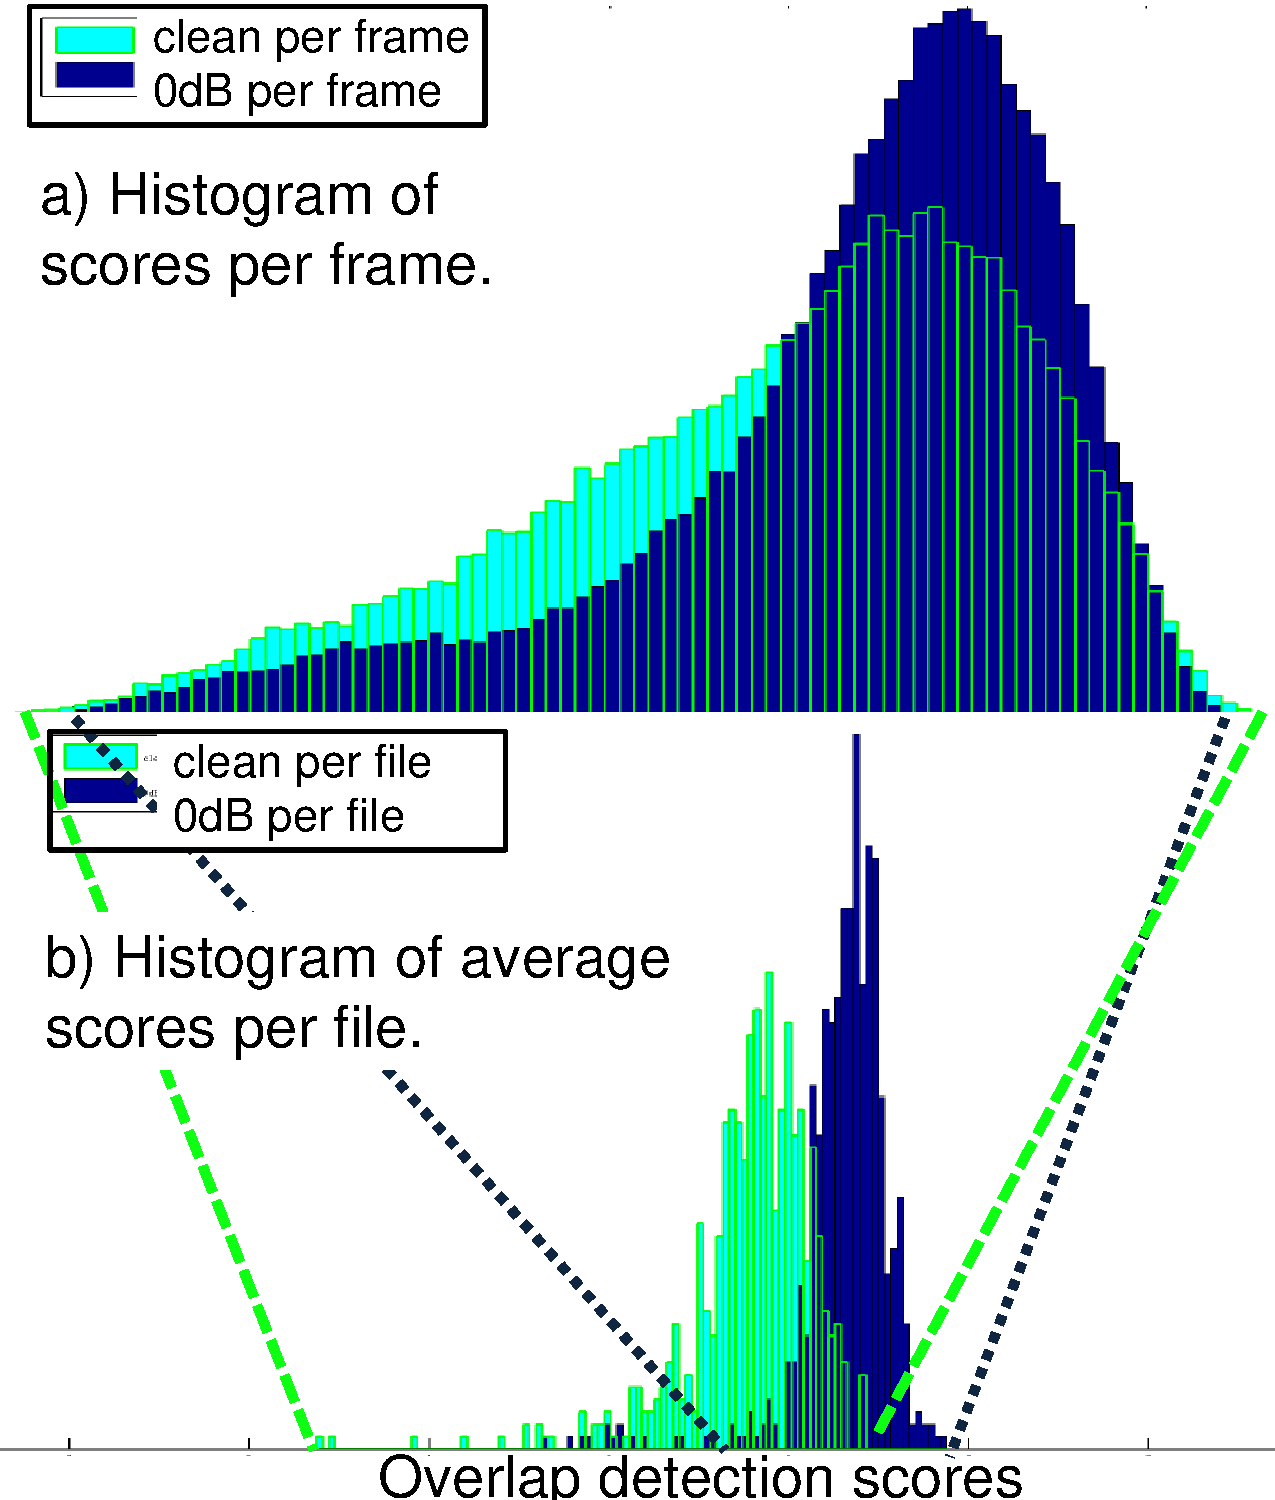
\includegraphics[height = 4in, width=0.5\textwidth]{figures/compare_pframe_pfile_hists}
	\vspace{-1mm}
	\caption{The effect of ensemble decisioning on distinguishability of overlapped regions. a) shows score per frame histograms and b) shows the histogram of ensemble scores. Using multiple frames to make a decision helps separate the distributions of clean and overlapped segments.}
	\vspace{-2mm}
	\label{fig:compare_perframe_and_perfile_ovldethist}
\end{figure}


%\subsection{HMM-based harmonic tracking for overlap detection}
%A more elaborate setup to track harmonic trajectories involves using a hidden Markov model (HMM) to model Pyknogram patterns. This allows for a supervised classification of speech segments into overlap and single-speaker speech. To do so, we propose using an initial segmentation of a given audio stream based on the Bayesian Information Criterion (BIC segmentation)~\cite{BIC}. The shorter segments are then compared against two pre-trained HMMs, one for overlapped and the other for single-speaker speech. The initial BIC segmentation is to allow for detection on shorter segments, since overlapped speech is considerably less frequent in a conversation compared to the total amount of speech. The combination of BIC segmentation and HMM-based classification allows for a practical overlap detection mechanism that fits well with analyzing conversations recorded in real conditions (as opposed to artificial datasets with simulated overlaps). Among other benefits of this framework is its compatibility with speaker diarization tools in which overlapped speech is considered a nuisance (see Sect.~\ref{sec:intro}). 

\newpage

\subsection{Evaluation}
\label{sec:exp}

This section evaluates our proposed pyknogram-based overlap detection system in terms of {\it accuracy, robustness,} and {\it precision}. 
Evaluation tasks for each SIR category are in the form of standard binary classification problems, where target examples are from a collection of files with fixed SIR values and non-target files are clean (single-speaker) files. 
We measure system performance using detection equal error-rates (EER; where false-positive and false-negative errors are equal). 
EER values are presented in Fig.~\ref{fig:ovl_det} for different SIRs. 
The expectation is that the detection algorithm should be consistent across a range of SIR values (i.e. robustness). 
As for precision, we are interested to know how short signals can be before overlap detection performance significantly drops (noting the observation in Fig.~\ref{fig:compare_perframe_and_perfile_ovldethist}). 


Bellow, a collection of overlap detection features are presented that have previously been used to detect overlapped regions~\cite{nav_icassp13,boakye_thesis,sapvr_2000}. 
%We note that all features were implemented based on the information provided in the publications, which are cited in each case. %adapted from other centers based on the information provided in publications. Although we tried to eliminate any chance of bias in the experiments, chances are that the results would have been different had the original authors implemented their methods for these experiments. 
To the best of our knowledge, overlap detection results on this database have not been reported for any of the following features, therefore we rely on our own implementations. %The out-of-house features used in this study are:


\subsubsection{Baseline features}

\label{ssec:baseline}
\begin{itemize}
  \item {\it Speech kurtosis}: Kurtosis has been reported as an effective measure to detect the presence of multiple speakers in overlapped signals by several studies~\cite{Wrigley_05,boakye_thesis,temple_kurtosis}. 
  It has been shown that overlapped speech exhibits lower kurtosis compared to single-speaker speech~\cite{leblanc_deleon98}. The kurtosis of a zero-mean random variable $x$ is defined as:

\begin{equation}
\label{eq:kurtosis}
k_x = \frac{E\{x^4\}}{(E\{x^2\})^2}
\end{equation}
\vspace{1mm}
In this case $x$ refers to speech samples in a given frame. 
  \item {\it Spectral flatness measure (SFM)}: The ratio of geometric to arithmetic means of spectral magnitudes across frequency within each frame~\cite{nav_icassp13}. For the $i^{th}$ frame:
\begin{equation}
\label{eq:kurtosis}
sfm_i = \frac{\frac{1}{N}\sum_{n=1}^{N}{X(f_n)}}{^N\sqrt{\prod_{n=1}^{N}{X(f_n)}}}
\end{equation}
\vspace{1mm}
where $X(f_n)$ corresponds to the magnitude spectrum at frequency $f_n$ and {N} is the total number of frequency bins. 
  \item {\it Spectral autocorrelation peak-valley ratio (SAPVR)}: described briefly in Sec.~\ref{sec:intro}, this feature uses the dominance of peaks in the spectral autocorrelation in each frame as a measure to detect overlaps~\cite{sapvr_2000}. 
\end{itemize}

\subsubsection{Data: Monaural Speech Separation Challenge}

The data used in our controlled experiments is from the monaural speech separation and recognition challenge (a.k.a speech separation challenge (SSC))~\cite{cooke20101}. 
The objective there was to permit a large-scale comparison of techniques for the overlapped speech problem~\cite{cooke20101}. 
Participants were asked to identify keywords in sentences spoken by a target talker when mixed into a single channel with a background talker speaking sentences of the same structure but with different content. 
The data used in SSC was obtained from the larger GRID corpus~\cite{cooke_JASA_SSCD}, which is a multi-talker audio-visual sentence corpus that supports computational-behavioral studies in speech perception. 
In our study, we only use the audio content which consists of 1000 sentences spoken by each of 34 talkers (18 male, 16 female). The sentences are structured in the following format.
\\\\
{\small \bf \textless command\textgreater\textless color\textgreater\textless preposition\textgreater\textless letter\textgreater\textless number\textgreater\textless code\textgreater}
\\\\
For example, ``lay white at X six now''.

The test and training set contain the same set of talkers. Seven overlapped sets are available, one clean and the rest composed of sentence pairs artificially summed at 6 signal-to-interference ratios (SIR) (+6, +3, 0, −3, −6, −9 dB). 
Since file durations are short (typically less than 5 seconds) and the utterances contain negligible pauses, it is reasonable to consider the average SIR values, provided for each file, a fair representation of the amount of overlap. 
This also allows the assumption that the entire signal is overlapped (see Fig.~\ref{fig:overlap_example}). 
We have down-sampled all files to 8kHz to match telephone recordings. 
Note that the experiments conducted in this study do not comply with the objectives of the speech separation challenge described in~\cite{SSC_link}. 

% Figure added because of Reviewer3 and 1's comment:
\vspace{0mm}
\begin{figure}[h!]
	\centering
	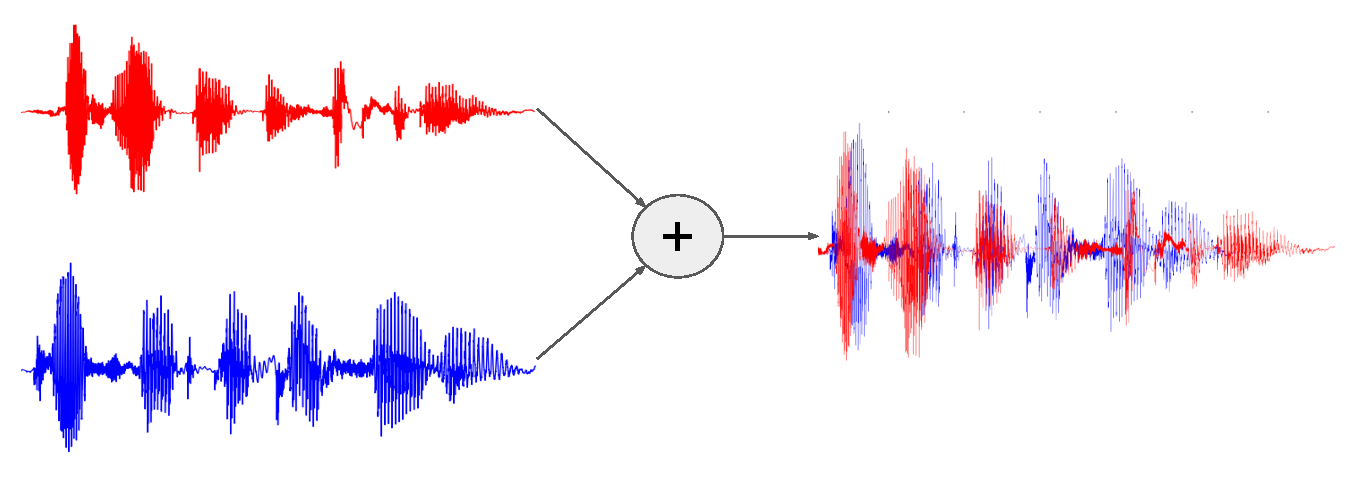
\includegraphics[height =1.8in, width=0.7\textwidth]{figures/GRID_example_overlap-crop}
	\vspace{-2mm}
	\caption{
		Example of the mixing process for a 0dB SIR overlapped signal. As shown on the right, it is fair to assume that overlap occurs throughout the signal.}
	\label{fig:overlap_example}
\end{figure}

% Reviewer1's comment:
This corpus is isolated from variabilities other than overlapped speech, which makes it useful to study the effects of overlap. 
To the best of our knowledge, this dataset is the most organized publicly available corpus that contains large, as well controlled, amounts of overlapped speech (note that we are mostly interested in {\it overlapped speech} and not {\it co-channel speech} as defined and distinguished in the introduction). 
Among the corpus' other advantages is the fact that segments are short which makes the definition of a signal-to-interference ratio more appropriate. Had the signals been longer, say a few minutes long, the notion of a signal-to-interference ratio across the entire signal would have been less applicable, due to the non-stationary nature of speech. 

\begin{table}[h!]
	\begin{center}
		\label{tab:data_summary}
		\begin{tabular}{| c | c |}
			\hline
			\hline
			number of speakers	& 18 (male)  \\
			\hspace{4mm}			&  16 (female) \\
			\hline
			average file duration	&   1.9 (sec) \\ 
			\hline
			noise				& interfering speakers \\
			\hspace{4mm}			& clean,$+6$, $+3$, $0$, $-3$, $-6$, $-9$ dB \\
			\hline
			sampling rate			& $8$ KHz \\
			\hline
			\hline	
		\end{tabular}
		\caption{Summary of data used for SID experiments}
	\end{center}
\end{table}


\vspace{3mm}
\subsubsection{Overlapped speech detection vs. SIR (Robustness \& Accuracy)}
Here the performance of pyknogram-based overlap detection is compared with the three baseline algorithms across different SIR values. 
The goal is to monitor the chances in EER as SIR values increase. 
The target/non-target files used in this binary classification task are obtained from a pool of overlapped and clean files. 
In each task, overlapped files with the same SIR are used as target examples and the overlap detection score (or feature value) assigned to them is compared against the scores estimated for clean files to compute the binary classification EER. 
Figure~\ref{fig:ovl_det} compares performances for the proposed and baseline systems across SIR values of $0, 3, 6$ and $9dB$.

\begin{figure}[h!]
	\centering
	\hspace{-1mm}
	\textbf{Overlap Detection vs. SIR}\par\medskip
	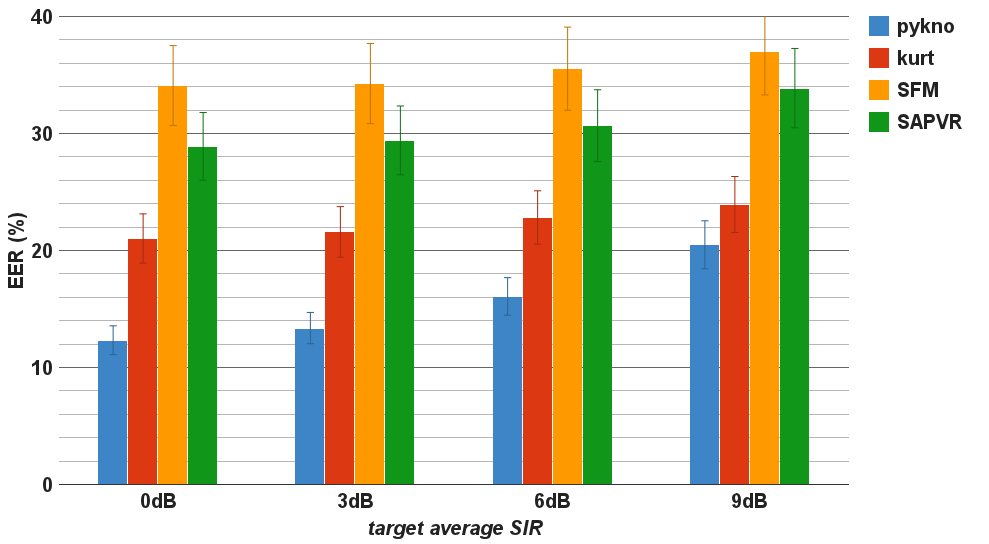
\includegraphics[height = 3.1in, width=0.7\textwidth]{figures/ovldet_vs_sir}
	\vspace{-1mm}
	\caption{Overlap detection EER for different SIR values. The higher the SIR, the more difficult it is to detect the presence of interfering speakers.}
	\vspace{0mm}
	\label{fig:ovl_det}
\end{figure}



\newpage
\subsubsection{Overlapped speech detection vs. segment length}
A main concern in dealing with overlapped regions is that overlap decisions are less reliable as segment lengths become shorter. 
This restricts algorithm precision in terms of the ability to detect overlap in a frame-based framework. 
Precision is most valuable in tasks such as speaker diarization in conversational speech, where overlap mostly occurs at speaker transitions in turn-takings. 
The goal of this phase is to evaluate system precision and compare pyknogram-based detection with baseline features. 
In other words, how short can overlap segments get before observing a significant drop in system performance. 
Once again, overlap detection performance is measured through the detection EER. 
Figure~\ref{fig:ovl_det_precision} shows the change in system performance as shorter duration segments are used to obtain overlap decisions. 


\begin{figure}[h!]
	\centering
	\hspace{-1mm}
	\textbf{Precision of Overlap Detection methods}\par\medskip
	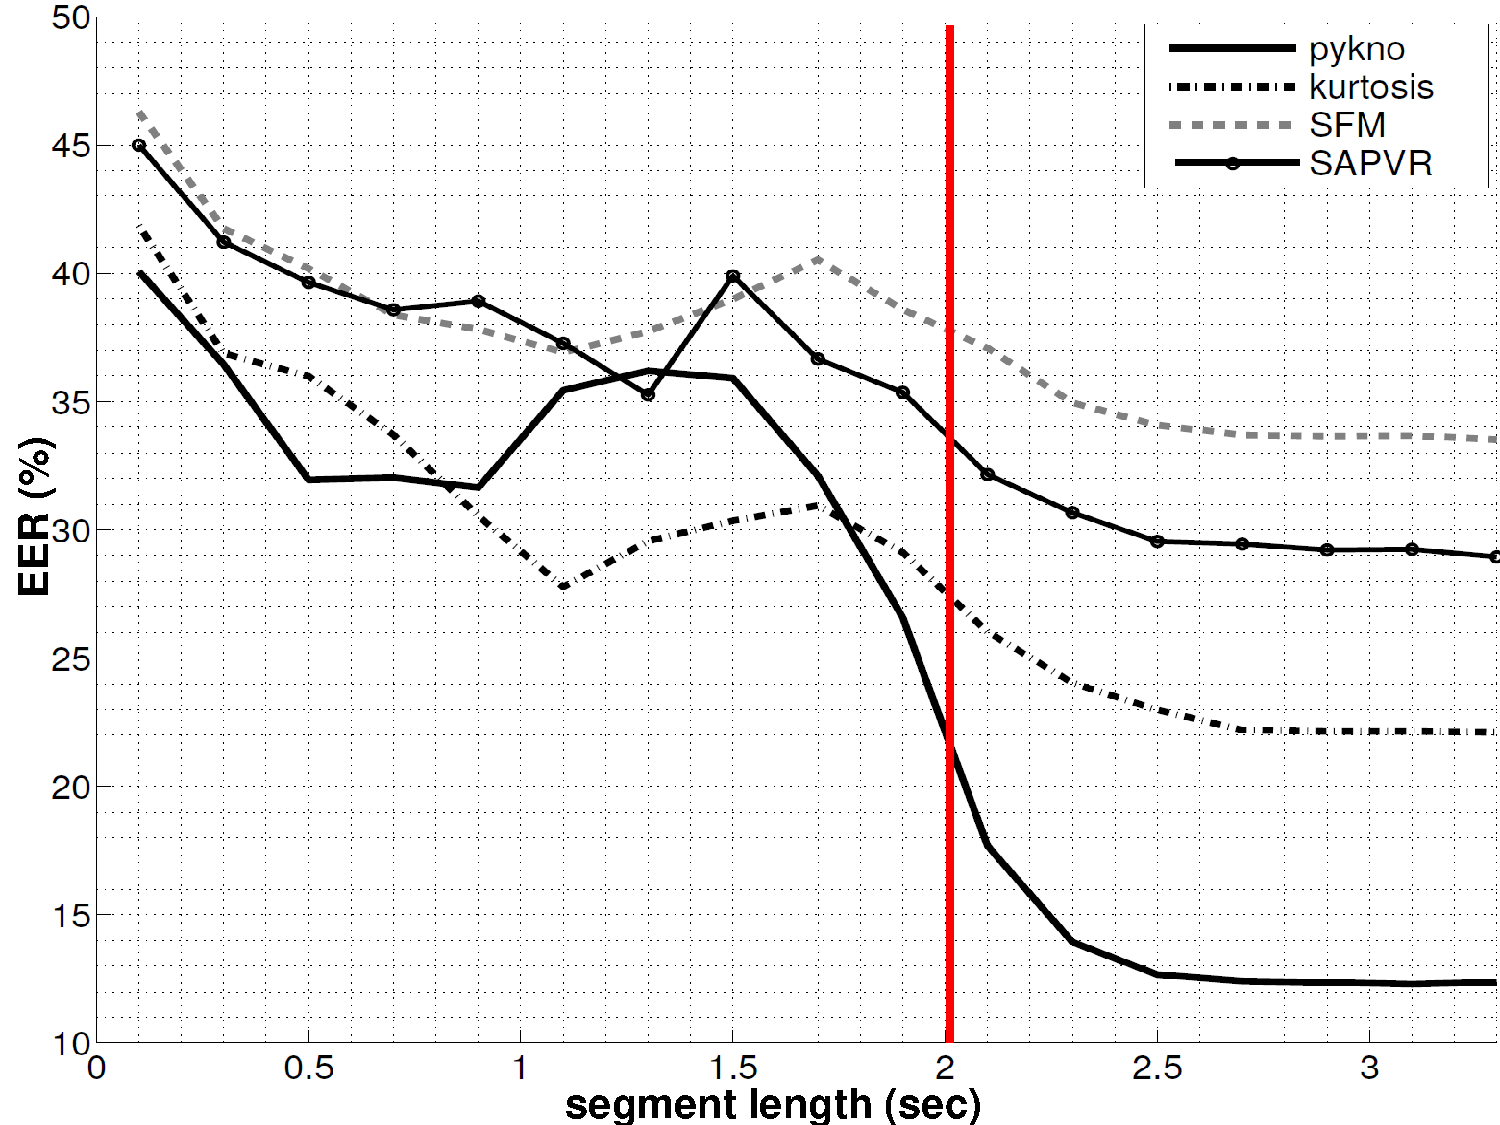
\includegraphics[height = 3.1in, width=0.5\textwidth]{figures/eer_vs_time}
	\vspace{-1mm}
	\caption{Overlap detection EER as a function of segment length. The plot shows that signal lengths should be at least $2$ seconds for the algorithms to start reaching their best performance.}
	\vspace{0mm}
	\label{fig:ovl_det_precision}
\end{figure}


\section{Gammatone Sub-band Frequency Modulation Spectra}
\label{sec:GSFM}



\chapter{SPEAKER RECOGNITION IN OVERLAPPED SPEECH}
\label{chapter:ovl_in_sid}
Detecting overlapped segments has previously been considered in speaker recognition diarization~\cite{boakye_thesis,yantorno_report}. 
In such problems, the presence of a secondary speaker either decreases model reliability (in training), or introduces confusion in the decision-making process by distorting test files. 
Overlap detection is computationally advantageous when compared to enhancing the desired speaker's speech. 
This approach is especially useful when one has the luxury of neglecting overlapped data~\cite{yantorno_report}. 
Such is the case for speaker recognition and diarization~\cite{Boakye_is_08}. 
By detecting overlapped speech segments, we are able to remove them from the training and decision-making process. However, overlap removal will not be the approach of choice in this chapter. 

As pointed out in Chapter~\ref{chapter:front-end}, the downside in removing overlapped segments is that a considerable amount of ``usable'' speech is also omitted from the speaker recognition system. 
An alternative solution is investigated in this chapter. 
In this solution, instead of directly applying overlap detection to data, overlap detection decisions are used as quality measure scores to assist speaker verification performance. 
This method is investigated in Sect.~\ref{sec:ch2_OvlQualityMeasure}. 
The primary contribution of this study is therefore to:
\begin{itemize}
	\item investigate overlap detection scores as quality measures for speaker verification. 
\end{itemize}
But first, this chapter begins by demonstrating the effects of overlapped data on speaker verification experiments (Sect.~\ref{sec:ch3_SIDintro}). 
This will provide an understanding of how overlaps affect speaker recognition. 
In addition, we will see how introducing overlaps to speaker verification affects train and test data separately (Sect.~\ref{sec:ch3_OvlinTest}~and~\ref{sec:ch3_OvlinTrain}). 


\section{Investigative setup}
\label{sec:ch3_SIDintro}
In order to show the detrimental effects of adding overlapped data to speaker verification, a case study is presented to analyze speaker recognition on data from the monaural speech separation challenge described in Chapter~\ref{chapter:front-end}~\cite{cooke20101}. 
Experiments use $12$-dimensional MFCC features ($13$ excluding the $0^{th}$ coefficient) plus $\Delta$ and $\Delta\Delta$, which together result in $36$-dimensional features. 
The experiments use the Gaussian mixture model (GMM) approach where a trained speaker is modeled using a mixture of Gaussians and the maximum likelihood of a given test audio file is computed from the train model. 
GMM parameters are obtained through maximum a-posterior adaptation of the parameters of a speaker independent GMM (called a universal background model which is trained on a large pool of speakers). 
Only GMM means are MAP-adapted in these experiments. 
$512$ mixtures were used to form the Universal background model (UBM). 

The next section slightly digresses from overlapped speech and is intended for readers unfamiliar with speaker recognition frameworks. 
Readers that feel comfortable with the concepts of speaker verification, specifically the use of GMM-UBM setups for speaker for verification, may skip Sect.~\ref{ssec:ch3_GMMUBM}.

As mentioned above, trials are generated from train and test sets designed for the speech separation challenge. 
The amount of clean (i.e., single-speaker) training data for each speaker is approximately $15$ minutes. 
Test data are provided in six SIR conditions, which are evaluated separately (see Sect.~\ref{sec:ch3_OvlinTest}). 
The challenge also provides overlapped training data. 
Overlapped training data are used in Sect.~\ref{sec:ch3_OvlinTrain} to train speaker models with the main speaker (i.e., model speaker in each train file) as the primary speaker and interfering speech from another randomly selected speaker. 
Experiments are gender-dependent, therefore the number of female speakers and male speakers is slightly different. 
In total over $10000$ trials are used to calculate equal error rates for each SIR condition presented in Sect.~\ref{sec:ch3_OvlinTest} and Sect.~\ref{sec:ch3_OvlinTrain} with a target to non-target ratio of $0.001$. 

\subsection{Speaker verification in a GMM-UBM setup} 
\label{ssec:ch3_GMMUBM}
The speaker verification problem is a manifestation of the more generic problem of speaker recognition in the form of a binary detection problem. 
Speaker recognition, taken literally, implies sufficient knowledge of all speakers (or at least a large number of speakers) to ``recognize'' a given speaker from his/her voice. 
Speaker verification, on the other hand, tackles the more manageable problem of determining whether an audio segment was produced by a known speaker. 
A speaker verification system usually produces a likelihood value for each verification task (aka trial). 
The collection of trial likelihood values produces two distributions, one of which corresponds to true (aka target) trials and the other to imposter (aka non-target) trials. 

The described framework requires a model for the training speakers (for whom we have several recording sessions available), but for the test speakers we only use the features from a test audio signal to compute the maximum likelihood (ML) probability of the test speaker belonging to the corresponding train speaker in each trial. 
Figure~\ref{fig:speaker_verification} summarizes a speaker verification setup. 

\begin{figure}[h!]
	\centering
	\vspace{0mm}
	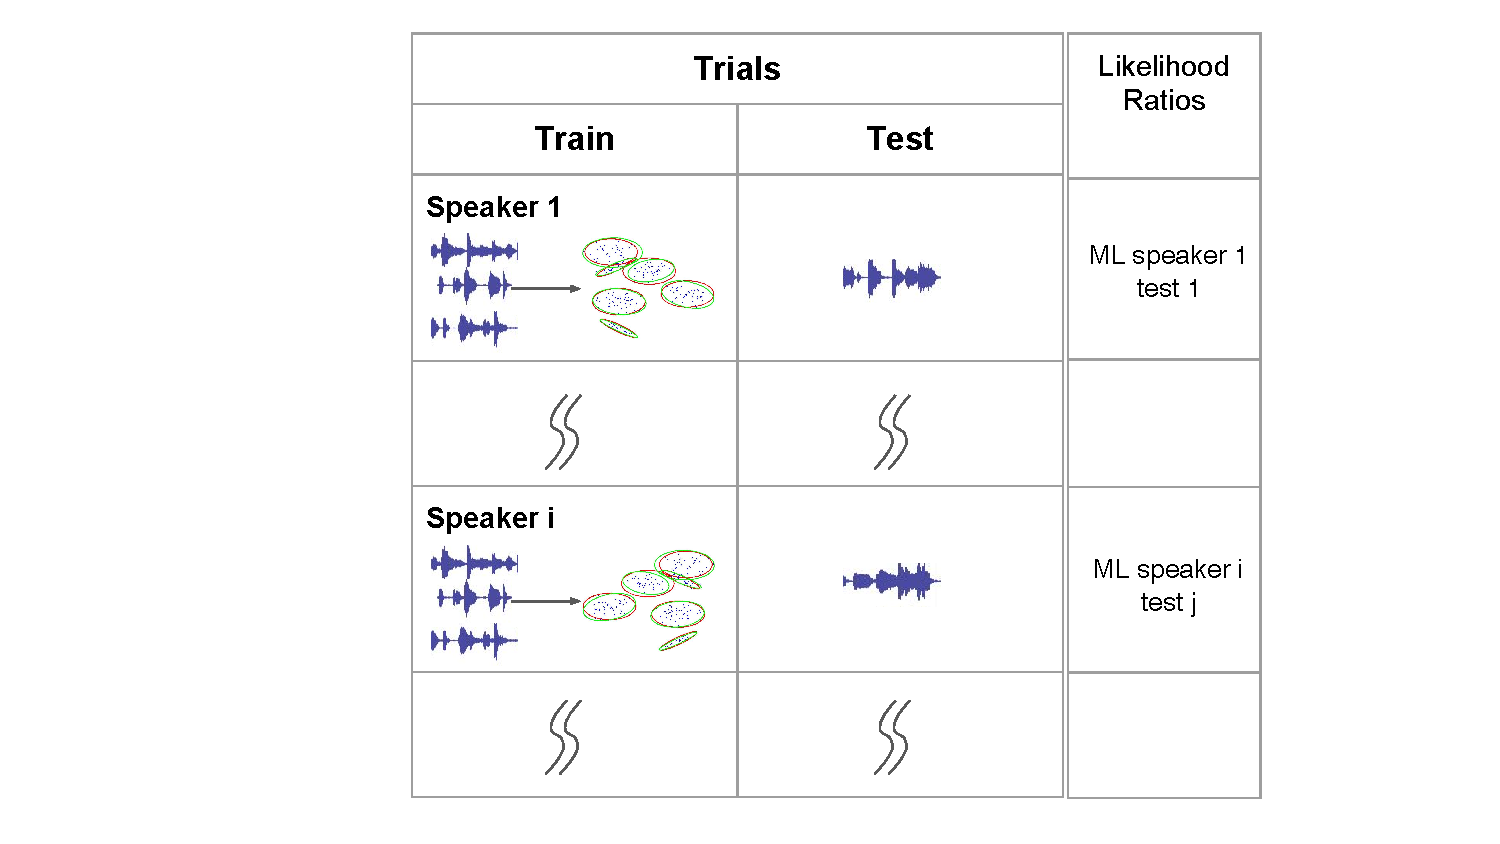
\includegraphics[height = 3in, width=0.8\textwidth]{figures/speaker_verification_setup}
	\vspace{-3mm}
	\caption{\it Speaker verification setup}
	\label{fig:speaker_verification}
	\vspace{0mm}
\end{figure}

The method through which likelihood ratios are calculated varies depending on the choice of model and system specifics. 
In the experiments presented in the following section, we use a GMM-UBM system~\cite{reynolds_map}. 
As mentioned above the task of the verification system is to calculate the likelihood of a test audio belonging to a speaker model. 
In other words, if the test audio belongs to speaker $i^\prime$ and the model (i.e., training speaker) belongs to speaker $i$, the objective is to calculate the likelihood of $i=i^\prime$. 
Here, a model is a Gaussian mixture model (GMM) obtained by adapting means of a universal GMM (aka UBM). 
The UBM is trained on background development data. 
In the examples provided in Sect.~\ref{sec:ch3_OvlinTest}~and~\ref{sec:ch3_OvlinTrain}, the development data is TIMIT. 
The verification system considers to hypotheses: 1) the probability of the test audio being generated from $GMM_i$, 2) the probability of the test audio generated from the UBM, which in this case represents every other speaker except $i$. 
The ratio between these two ratios is used to quantify the system decision for a given trial. 
Figure~\ref{fig:gmm_ubm_sid} illustrates the procedure to determine the likelihood ratio for one trial. 

\begin{figure}[h!]
	\centering
	\vspace{0mm}
	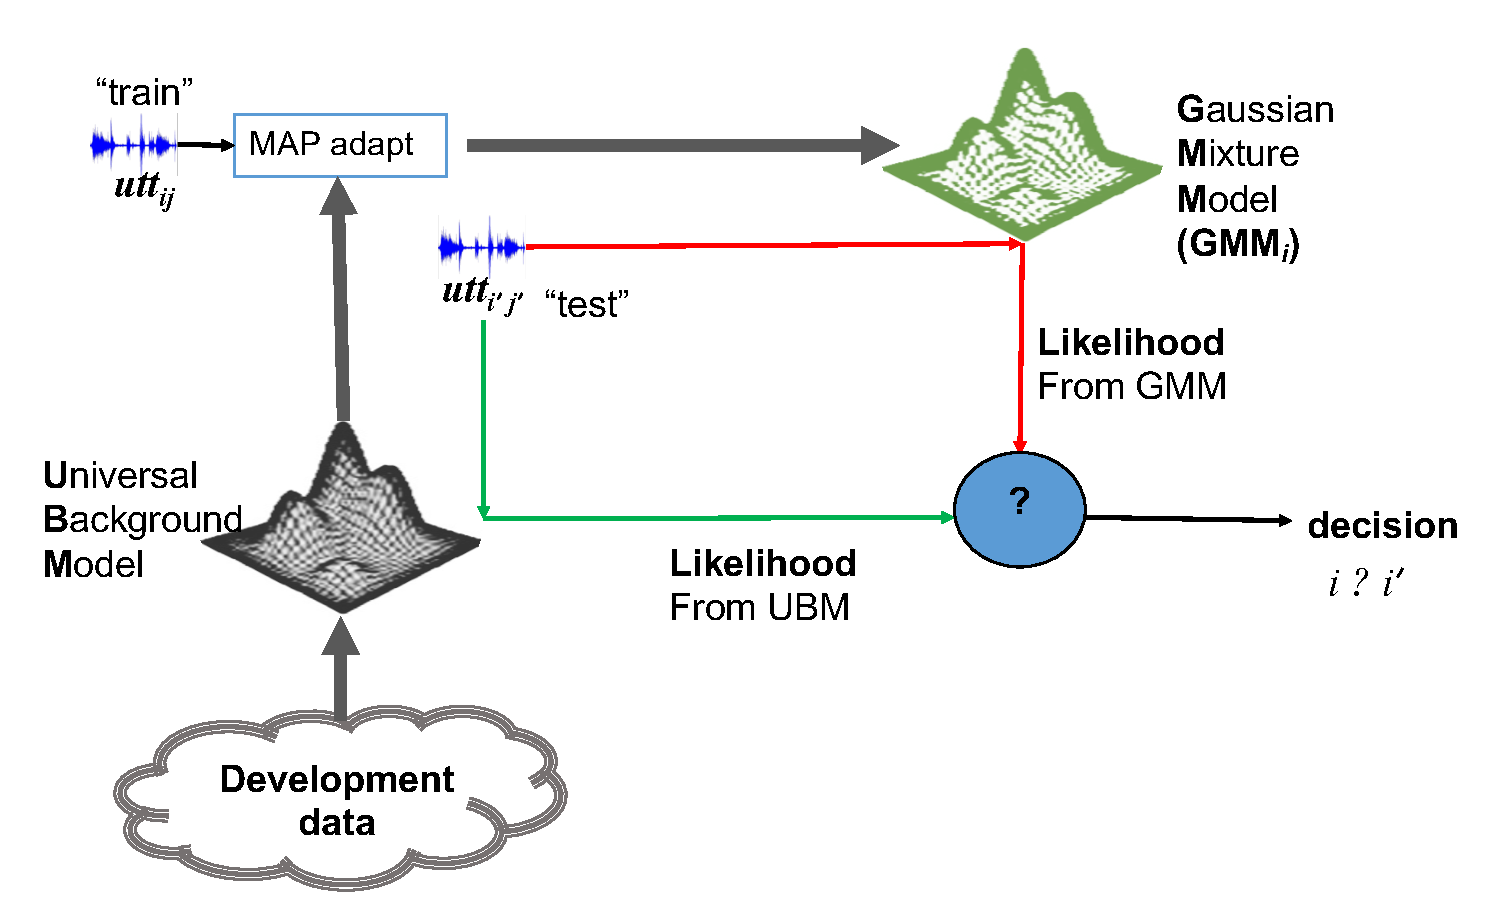
\includegraphics[height = 3.5in, width=0.9\textwidth]{figures/gmm_ubm_sid_setup}
	\vspace{-3mm}
	\caption{\it Speaker verification setup}
	\label{fig:gmm_ubm_sid}
	\vspace{0mm}
\end{figure}

Given this introduction, we expect that the reader should now be able to follow the remainder of this chapter. 
Useful descriptions of topics on speaker verification and recognition can be found in~\cite{hansen2015SIDmagazine}. 


\section{Overlaps in test data}
\label{sec:ch3_OvlinTest}
As a comparison benchmark, performance is evaluated under clean train and test conditions on the SSC data. 
Gaussian mixture models (GMM) are adapted from a Universal back model (UBM) trained on TIMIT files~\cite{msridentity}. 
For each model (training) speaker, there are 500 utterances in SSC, which are all used in the training process. Test files are available in all SIR conditions. 
As expected, lower SIR values correspond to higher equal error rates. 
The presence of a secondary speaker, clearly causes confusion in the score distribution, leading to less separability between target and imposter trials. 
recognition performance under clean test files and those with average SIR ranging in $+6, +3, 0, -3, -6, -9 dB$ are provided in Fig.~\ref{fig:sidingrid_ovlintest_train_a}. 

It is worth mentioning that it was tempting to compare these results with stationary noise experiments. 
However, contrary to expectations, it was observed that performances were better in the overlapped condition when compared to white Gaussian noise and speech-shaped noise interference, even for negative SIR values. 
This is most likely due to a misunderstanding caused by comparing stationary and non-stationary noise through the same measurement procedure, which is the SIR (or SNR). 
For a given target speech file, adding a certain amount of stationary noise will affect all frames, whereas in the case of non-stationary noise (here speech) only a portion of the frames receive non-uniform interference. 
This leads to incomparable results under presumably similar conditions which we decided to exclude from this study to avoid confusion. 
Therefore, an important take-away message here is that a certain {\bf SIR} value does not translate to the same {\bf SNR}. 


\section{Overlap in train data}
\label{sec:ch3_OvlinTrain}
This section examines the effect of adding overlapped speech to train files (Fig.~\ref{fig:sidingrid_ovlintest_train_b}). 
Figures~\ref{fig:sidingrid_ovlintrainvstest_male} and \ref{fig:sidingrid_ovlintrainvstest_female} compares the effects of adding overlapped speech in train and test files. 

An interesting observation is the higher rate with which the EER increases when the SIR drops for the test condition. 
We believe this is due to the fact that in train conditions, the training of Gaussian mixture models tends to cancel out the effect of the interfering speech. 
For each speaker, the GMM is trained on a set of features, some of which are influenced by the desired speaker and the rest influenced by the interfering speakers. 
Since multiple training files are used to model each speaker (different training files have different interfering speakers), the GMM tends to converge to a common locale in the feature space, which belongs to the speaker for whom the models are being trained. 
We call this effect averaging out (or cancelling out) of the interfering speakers. 
This to some extent slows the growth in EER as the data becomes noisier in train files. 
Such cancellation, however, does not exist across test files.



\begin{figure}[h!]
	\centering
	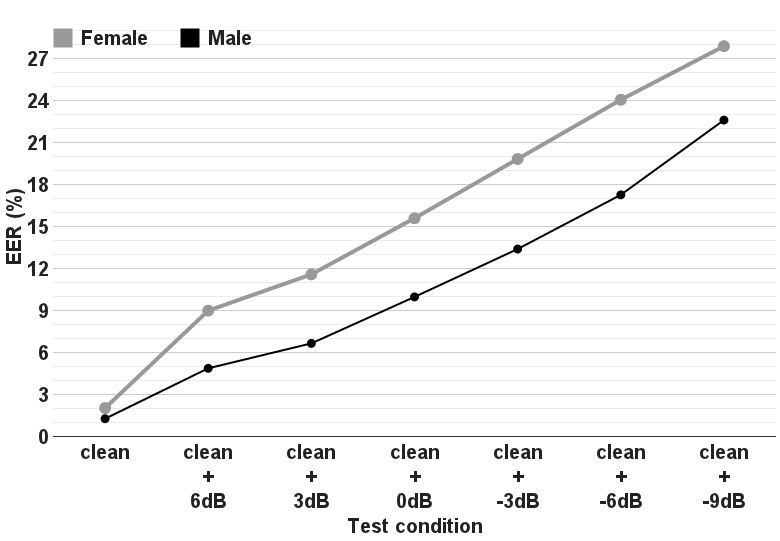
\includegraphics[height = 3.43in, width=0.9\textwidth]{figures/sidingrid_ovlintest}
	\vspace{-1mm}
	\caption{\it The rise in EER values as we increase the effect of overlapped speech (via decreasing the SIR). Starting from clean (i.e. single-speaker speech) to lower SIR values. a) Shows the case where train files are clean, but test files contain overlaps. }
	\label{fig:sidingrid_ovlintest_train_a}
\end{figure}
\begin{figure}[h!]%{0.5\textwidth}
	\centering
	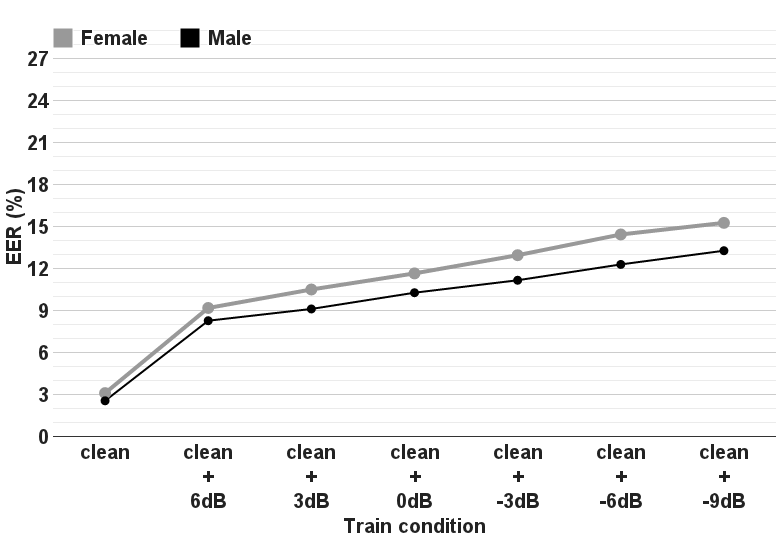
\includegraphics[height = 3.43in, width=0.9\textwidth]{figures/sidingrid_ovlintrain}
	\vspace{-1mm}
	\caption{\it b) clean test files but train files contain overlaps.}
	\label{fig:sidingrid_ovlintest_train_b}
\end{figure}



\begin{figure}[h!]
	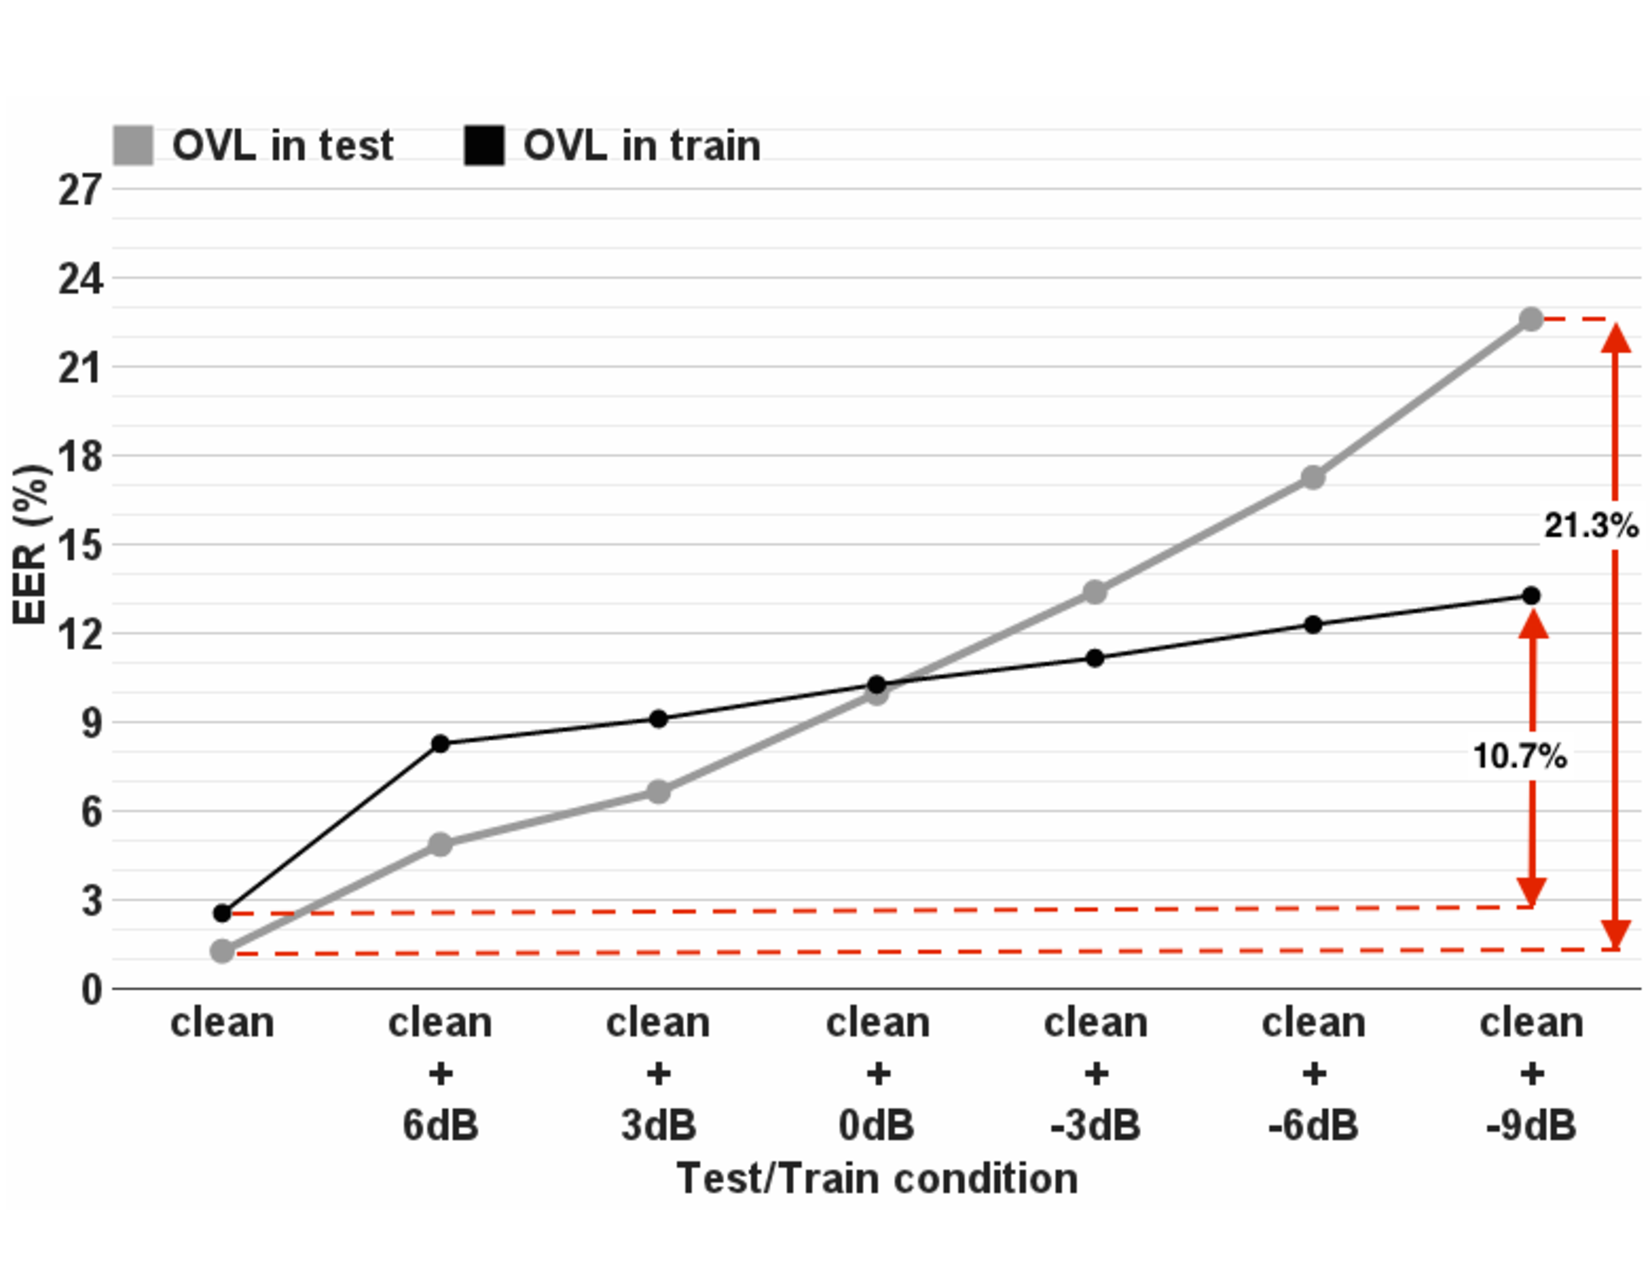
\includegraphics[height = 3.43in, width=0.9\textwidth]{figures/sidingrid_ovlintrainvstest_male_rev1}
	\caption{\it Comparing the impact of increasing overlap (OVL) in train vs. test data by decreasing SIR values. Experiments for male speakers (a). Lower SIR drops the performance more rapidly when applied to test data.}
	\label{fig:sidingrid_ovlintrainvstest_male}
\end{figure}

\begin{figure}[h!]
	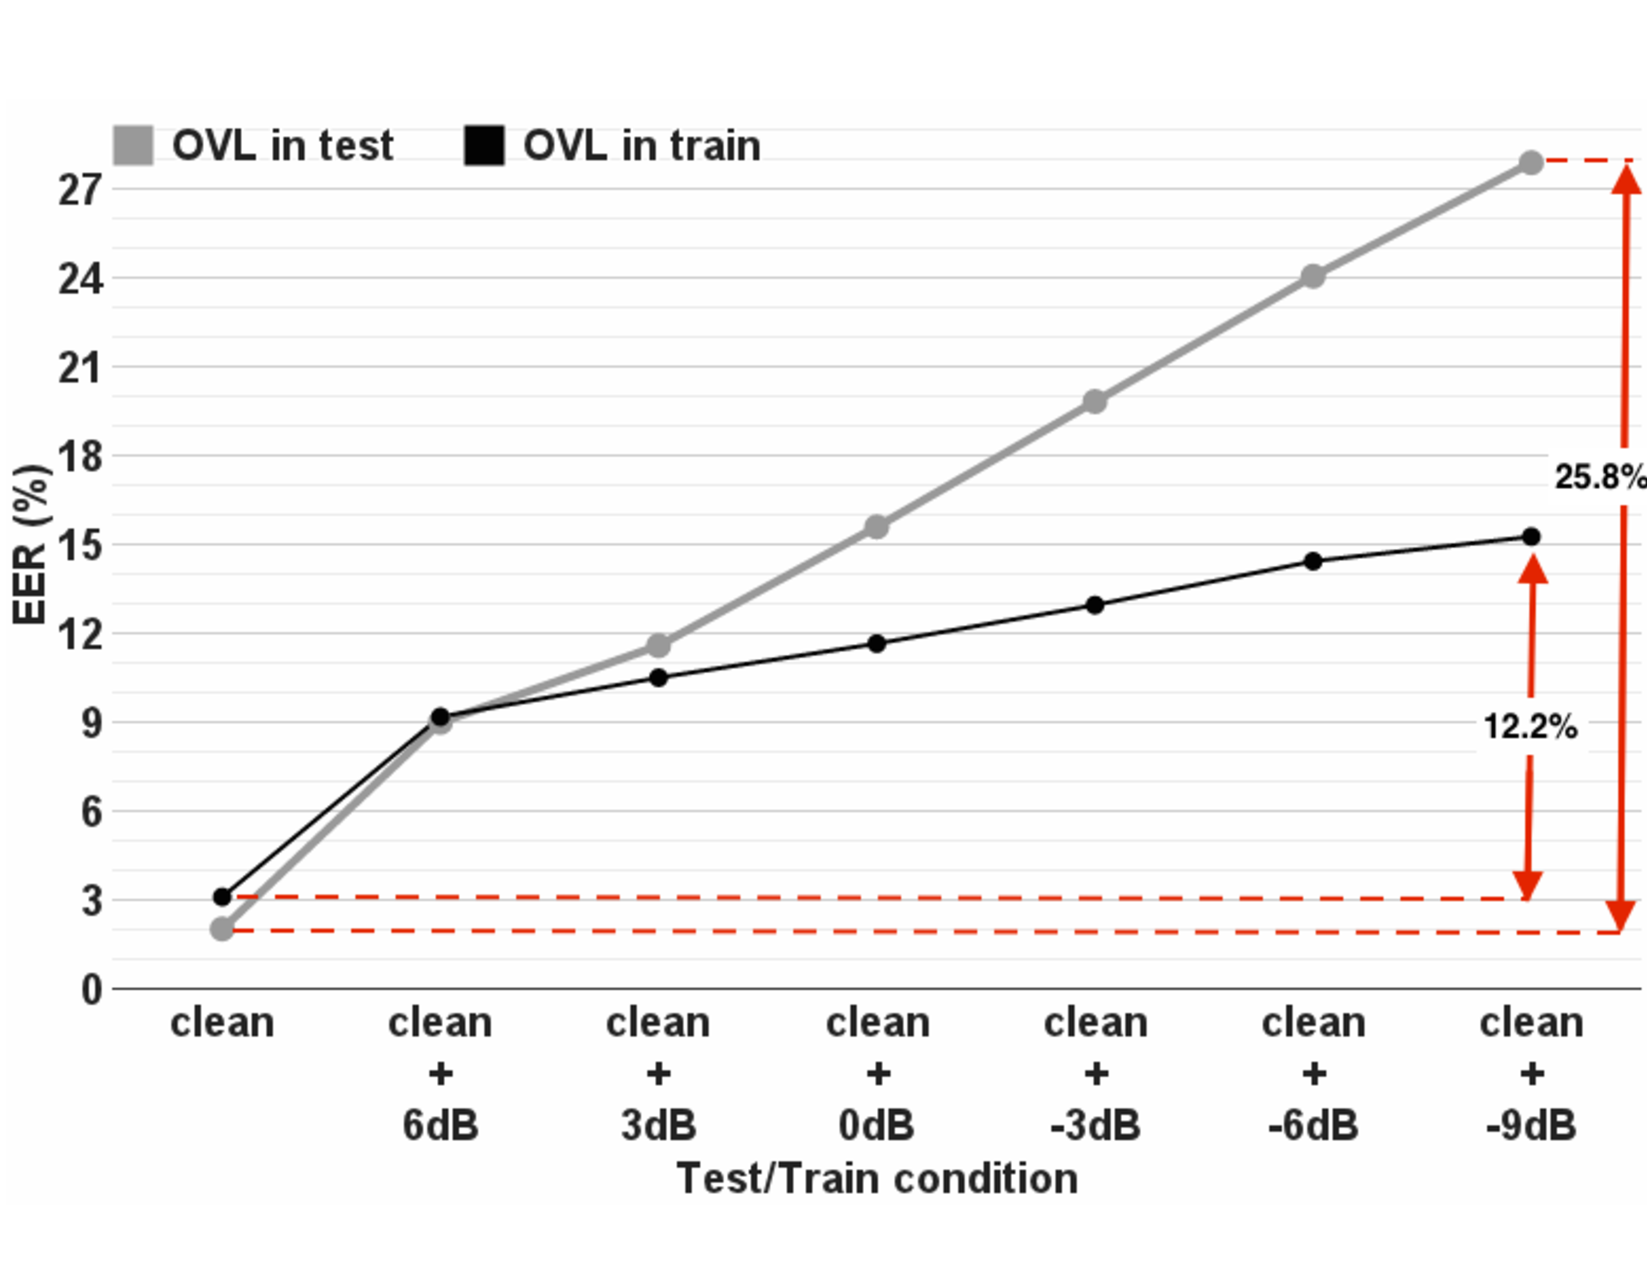
\includegraphics[height = 3.43in, width=0.9\textwidth]{figures/sidingrid_ovlintrainvstest_female_rev1}
	\caption{\it b) female}
	\label{fig:sidingrid_ovlintrainvstest_female}
\end{figure}


The results provided in Sect.~\ref{sec:ch3_OvlinTest}~and~\ref{sec:ch3_OvlinTrain} were provided to focus explicitly on the impact of overlaps on speaker verification. 
This is believed to be novel from two perspectives: 
1) The data used here is actually overlapped, meaning that files contain two speakers speaking at the same time, and not the generic case of co-channel. Therefore, the results provide greater motivation and direction as we move on to the next sections, which focus on overlap detection. 
2) The comparison made between adding overlap to test vs. training data provides insight in determining which (train or test) to prioritize for to remove overlap. Bare in mind that simply removing everything that is assumed to be overlapped does not necessarily yield optimal performance, since losing data lowers model reliability and the number of test features used to calculate likelihood values. 


\section{Overlap detection as meta-data for speaker recognition}
\label{sec:ch2_OvlQualityMeasure} 
Using meta-data to yield more accurate decisions is a common practice in speaker verification evaluations~\cite{bosaris,qual_sid_13}. 
Incorporating quality measures such as speech activity detection (SAD) and effective file durations can significantly improve verification performance~\cite{qual_sid_13,CRSSSRE12} regardless of system architecture (be it i-vector, GMM-UBM, or any other system). 
Quality measure refers to additional information (i.e. meta-data) used alongside speaker verification likelihood ratios (aka speaker verification scores) to quantify the test and train conditions in trials. 
Meta-data provides lower-level scores that help increase distinguishability between target/imposter trials. 
For speaker verification in overlapped speech, the primary source of confusion is caused by the presence of interfering speakers. 
This section proposes to use scores from overlap detection algorithm(s) as secondary information to improve overall speaker verification performance. 

There are several approaches through which quality measures can be applied in a binary classification scenario~\cite{bosaris,ietqstack,kelly2013}. 
Here, we use a stacking approach, called Q-stack, in which the quality measures (here overlap decisions) are concatenated (i.e., ``stacked'') with speaker verification decisions~\cite{ietqstack}. 
The resulting vector is a high-dimensional score vector which allows more separability due to the additional information provided by the stacked dimensions. 
The stacked score vectors are then processed with a support vector machine (SVM) classifier. 
SVM parameters are trained using a development set extracted from a separate subset of the data. 
In experiments, the development set consists of $10,000+$ trials, a quarter of which are clean trials and the remaining $7,500+$ trials contain overlapped test files with $0,3,6dB$ SIR levels. 
The target to imposter ratio in speaker verification trials is $0.001$. 
An evaluation set of size $18,000$ trials with similar specifics and target-imposter ratio is used to test overall system performance.


Table~\ref{tab:sid_stack_results} shows the improvements obtained by using the overlap detection scores individually and combined. 
Kurtosis and SFM show less correlation, however they provide significant complementary information when combined and used alongside SAPVR and pyknogram features. 
The best result is obtained when all four features are concatenated, since each overlap detection system may yield better performance in certain scenarios.  


\begin{table}[t]
	\centering
	\begin{tabular}{|c|c|c|c|c|c|}
		\hline
		raw GMM/UBM scores & pykno & kurtosis & SFM & SAPVR & $\textit{\textbf{EER (\%)}}$ \\ \hline
		\cellcolor[HTML]{C0C0C0}{\color[HTML]{343434} } \checkmark &  &  &  &  & 11.36\\ \hline \hline
		\cellcolor[HTML]{C0C0C0} \checkmark & \cellcolor[HTML]{C0C0C0} \checkmark &  &  &  & 10.19 \\ \hline
		\cellcolor[HTML]{C0C0C0} \checkmark &  & \cellcolor[HTML]{C0C0C0} \checkmark &  &  & 13.51 \\ \hline
		\cellcolor[HTML]{C0C0C0}{\color[HTML]{343434} } \checkmark &  &  & \cellcolor[HTML]{C0C0C0}{\color[HTML]{343434} } \checkmark &  & 28.35 \\ \hline
		\cellcolor[HTML]{C0C0C0} \checkmark &  &  &  & \cellcolor[HTML]{C0C0C0} \checkmark & 9.48 \\ \hline \hline
		\cellcolor[HTML]{C0C0C0}{\color[HTML]{343434} } \checkmark & \cellcolor[HTML]{C0C0C0} \checkmark & \cellcolor[HTML]{C0C0C0}{\color[HTML]{343434} } \checkmark &  &  & 10.20 \\ \hline
		\cellcolor[HTML]{C0C0C0} \checkmark & \cellcolor[HTML]{C0C0C0} \checkmark &  & \cellcolor[HTML]{C0C0C0} \checkmark &  & 10.47 \\ \hline
		\cellcolor[HTML]{C0C0C0} \checkmark & \cellcolor[HTML]{C0C0C0} \checkmark &  &  & \cellcolor[HTML]{C0C0C0} \checkmark & 9.57 \\ \hline \hline
		\cellcolor[HTML]{C0C0C0} \checkmark & \cellcolor[HTML]{C0C0C0} \checkmark & \cellcolor[HTML]{C0C0C0} \checkmark & \cellcolor[HTML]{C0C0C0} \checkmark &  & 10.31 \\ \hline
		\cellcolor[HTML]{C0C0C0} \checkmark & \cellcolor[HTML]{C0C0C0} \checkmark & \cellcolor[HTML]{C0C0C0} \checkmark & \cellcolor[HTML]{FFFFFF} & \cellcolor[HTML]{C0C0C0} \checkmark & 9.18 \\ \hline
		\cellcolor[HTML]{C0C0C0} \checkmark & \cellcolor[HTML]{C0C0C0} \checkmark & \cellcolor[HTML]{C0C0C0} \checkmark & \cellcolor[HTML]{C0C0C0} \checkmark & \cellcolor[HTML]{C0C0C0} \checkmark & {\bf 9.10}\\ \hline
	\end{tabular}
	\caption{\it Speaker verification performance (EER) with and without overlap detection scores as meta-data. Grey cells highlight the features used in each experiment. The relative change in EER is presented in the last column.}
	\label{tab:sid_stack_results}
	\vspace{-5mm}
\end{table}

\vspace{0mm}

% The following paragraph was added after reviewer1's comments (and also reviewer 3):
Better individual performances from SAPVR and SFM is because they are superior in distinguishing harmonic structures. 
Since speaker identities are mostly influenced by voiced speech, this assists the speaker recognition task in quantifying the amount of reliable voiced segments. 
Pyknogram-based detection is designed to locate harmonic discontinuities as opposed to the presence of harmonics. 

Experiments show that the best performance is obtained using an SVM with a radial basis function (RBF) kernel. 
The SVM parameter(s) (here $\gamma$) are determined through cross-validation on the development set. 
Class weights (i.e., target/imposter weights for the SVM classifier) and the cost (aka slack) parameter are selected according to the detection cost function (DCF) parameters ($C_{fa}$, $C_{miss}$, and $prior$) used throughout experiments~\cite{bosaris}. %Table~\ref{tab:sid_stack_results}  The highest relative improvement is obtained when all features are concatenated. 

An additional experiment is also conducted using ideal overlap labels (labels from ground-truth) in the Q-stack paradigm which results in an lower bound in error rates.
The EER for this lower bound is $8.74\%$ ($23\%$ relative improvement). 
In the Q-stack algorithm, the relative drop in EER from using all overlap features is approximately $20\%$, which is not far off from when ground-truth labels are used. 
This confirms the effectiveness of the selected overlap detection features/scores.  
Using the proposed Pyknogram-based overlap detection system and baseline features the relative improvement is $20\%$, a mere $3\%$ lower than the best achievable performance provided by the lower bound.


\section{Summary}
\label{sec:ch3_summary}
Chapter~\ref{chapter:ovl_in_sid} provides an investigative study of overlapped speech in speaker recognition systems. 
This effect was measured by adding overlapped speech to training and test data in a speaker recognition problem. 
Since the focus in this chapter was on physical attributes of overlapped speech, all experiments were conducted on independent cross-talk data (as defined in Chapter~\ref{chap:intro}). 
It is shown that overlapped speech is more detrimental when added to test data, due to its impact on the final verification score. 
When overlap is added to training data, the effect of interfering speech is mitigated as the different secondary speakers are averaged out across training sessions provided for a given speaker. 
A proposed method to decrease the impact of overlapped speech is to use overlap detection scores as meta-data for a speaker verification system. 
The traditional approach has been to simply remove overlapped segments. 
Alternatively, this study investigates the improvement obtained by preserving data (be it overlapped or not) while calibrating speaker verification scores to adjust to various levels of overlap in test and training data. 



\chapter{Speaker Recognition in Co-channel Speech}
\label{chapter:backend}

%\begin{figure}[b]
%	\hrule
%	\vspace{.03cm}
%	{\rmfamily{\small \em { Mail All Correspondence To:}\vspace{-0.2cm}\\}}
%	\begin{minipage}{0.2\linewidth}
%		\centering
%		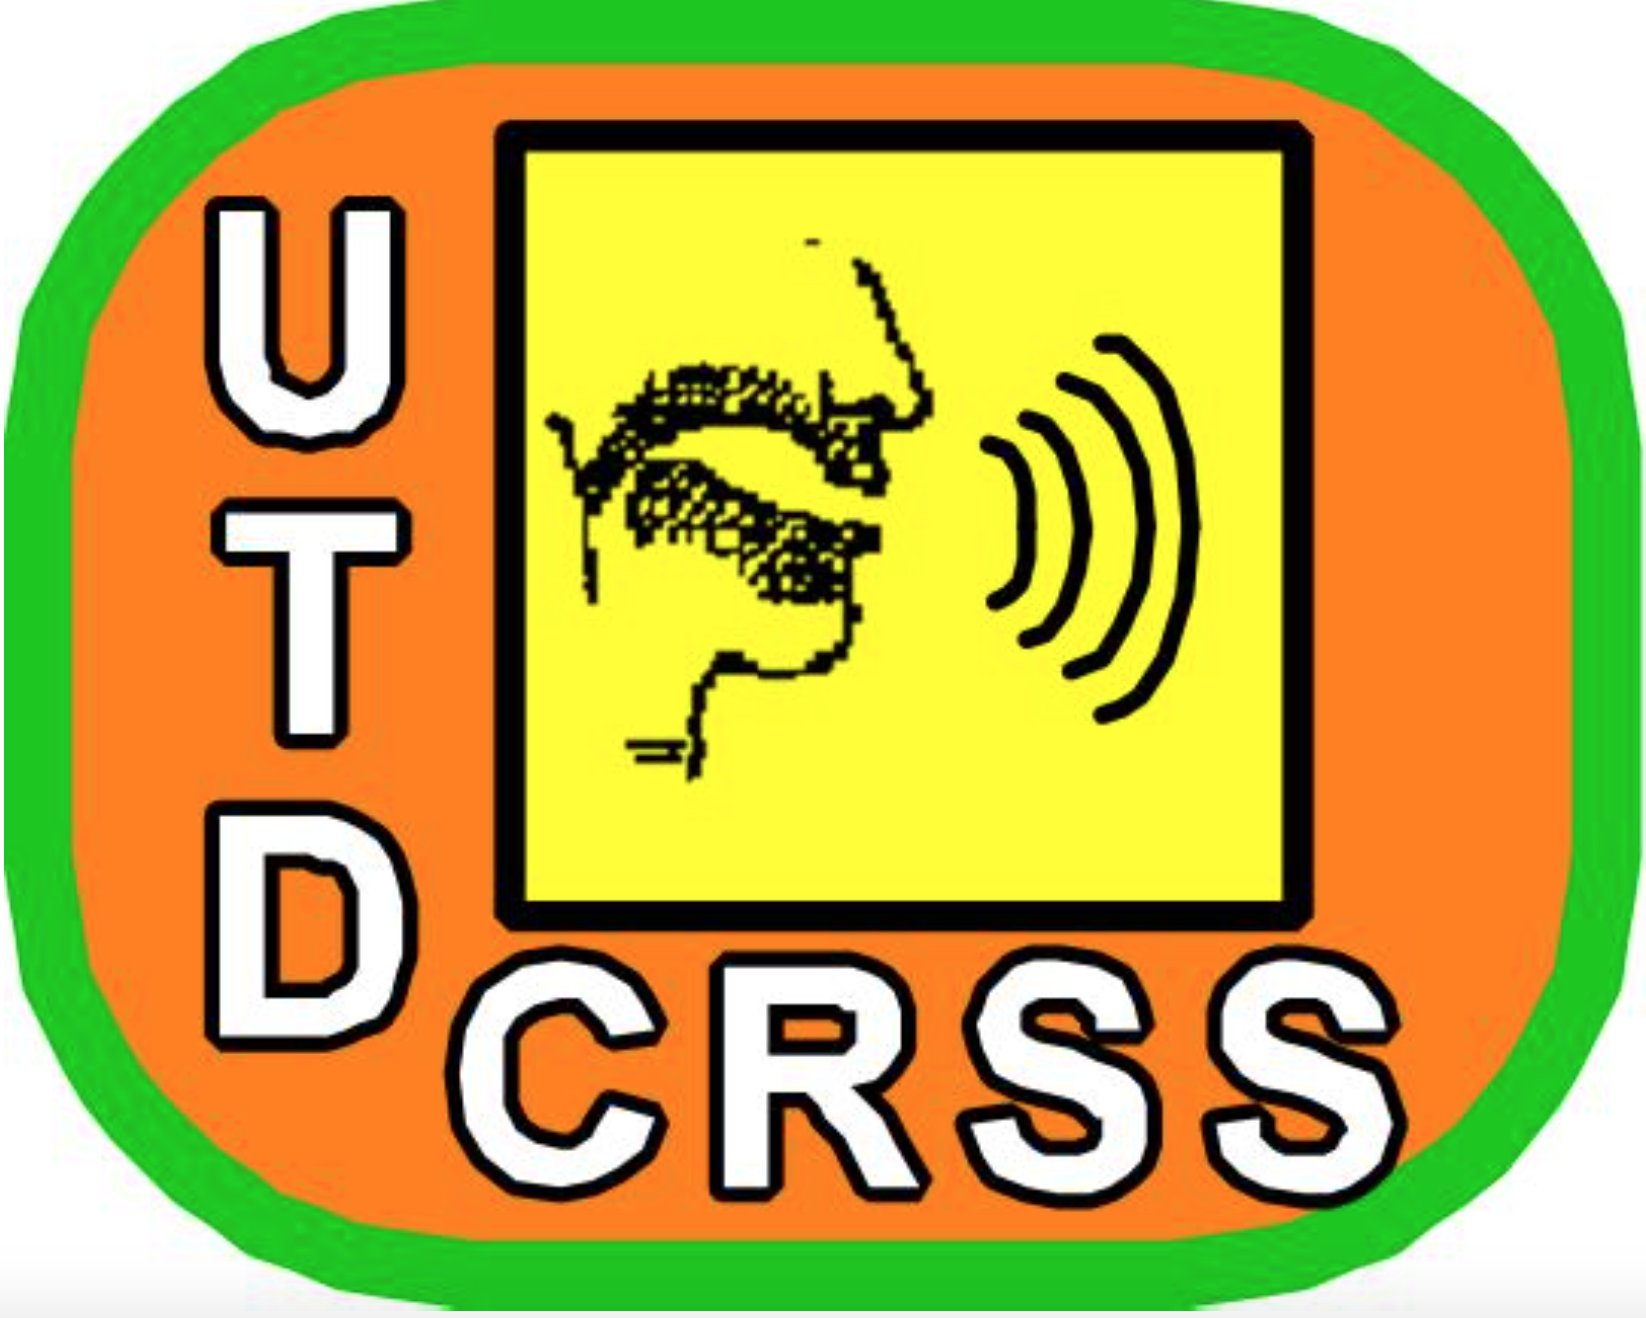
\includegraphics[width=1\linewidth]{chapters/cochannelplda_jp/IEEEtran/figures/CRSS_logo}
%	\end{minipage}
%	\begin{minipage}{0.8\linewidth}
%		\begin{singlespace}
%			\small \vspace{.5cm}
%			\footnotesize
%			Prof. John H.L. Hansen\\
%			Center for Robust Speech Systems (CRSS), Erik Jonsson School of Engineering and Computer Science, Dept. of
%			Electrical Engineering, University of Texas at Dallas\\
%			2601 N. Floyd Road, EC33, Richardson, TX 75080-1407, U.S.A\\
%		\end{singlespace}
%	\end{minipage}
%	\small{$^*$This project was funded by AFRL under contract FA8750-12-1-0188 and partially by the University of Texas at Dallas from the Distinguished University Chair in Telecommunications Engineering held by J.H.L. Hansen.}\\
%\end{figure}

This chapter addresses the problem of speaker recognition for co-channel recordings, rather than speaker recognition in overlap. 
The main focus is on interference from secondary speakers, be it overlapped or not. 
Secondary speech interference, the main characteristic of co-channel, is an important source of error for all automatic speech processing systems. Speaker recognition experiments are highly influenced by the presence of secondary speakers, due to reduced reliability of the trained models. 
Although the target speaker is a common factor in all training samples for a given speaker model, the standard structure of speaker recognition systems has not been designed to average out interfering speech. 

To the best of our knowledge, few studies address speaker recognition in co-channel speech signals. 
However, the effects of artificially adding {\bf overlapped speech} in a speaker verification setup has received considerable attention~\cite{yantorno_report,yantorno_SID,Dwang_03}. 
In many of these studies, the approach was to automatically detect and remove overlaps from co-channel speech in training and test data. 
Although many overlap detection algorithms have been investigated over the years~\cite{Boakye_icassp_08,nav_icassp13,smolenski_tut,sapvr_2000}, none have considered solving the problem in the more general case of co-channel interference. 

This chapter differentiates co-channel speech from overlapped speech by considering the latter a special case of the former where both speakers are active at the same time. 
Co-channel speech refers to the broader case where speakers are not necessarily overlapping (see Fig.~\ref{fig:cochannel_vs_overlap}). 
We focus on speaker recognition in co-channel speech interference, in which overlaps may occur.  
This sheds light on a more realistic problem, since only a small percentage of conversational speech contains amounts of overlap that are large enough to significantly lower speaker recognition performance~\cite{cetin_shriberg_06_icassp,smolenski_tut}. 

\begin{figure*}[t!]
	\centering
	\vspace{0mm}
	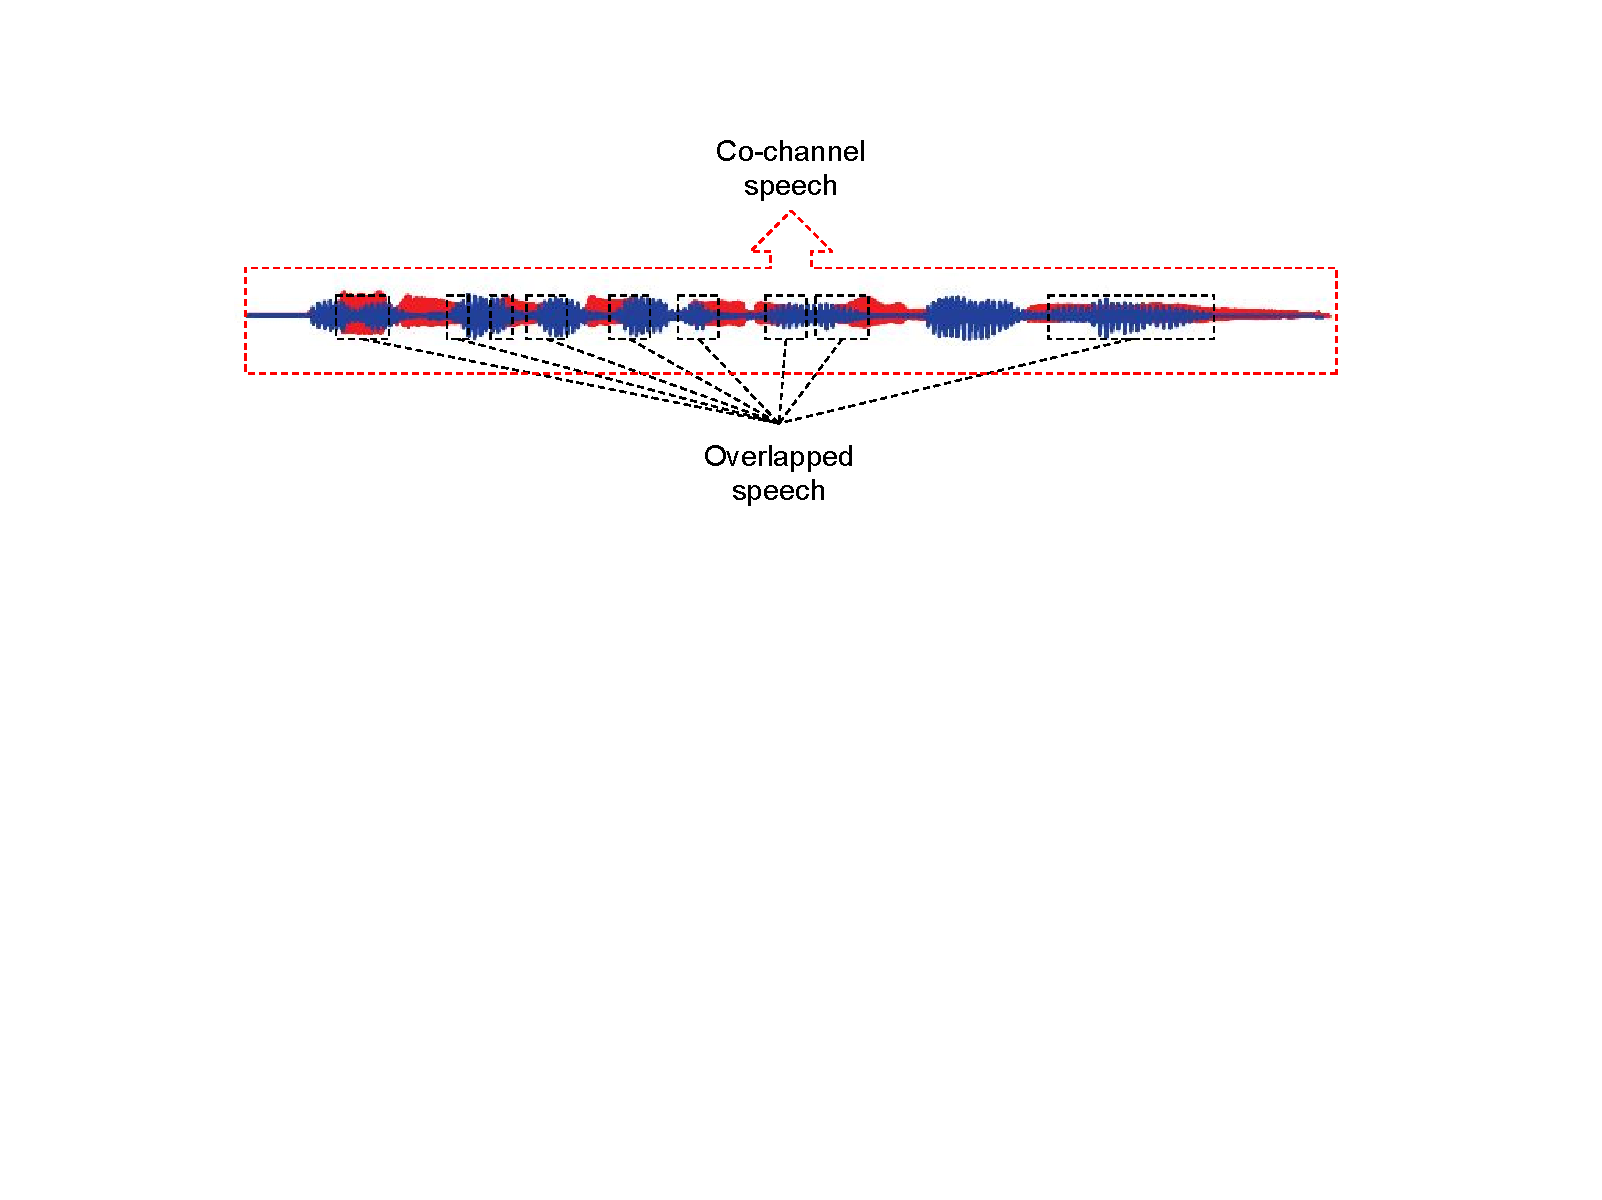
\includegraphics[height = 2in, width=0.9\textwidth]{figures/cochannel_vs_overlap-crop}
	\vspace{-3mm}
	\caption{\it \small Difference between co-channel and overlapped speech. Overlap refers to instances where more than one speaker is active. Co-channel is defined as an entire stream that contains multiple speakers. All co-channel files do not necessarily contain overlap. }
	\label{fig:cochannel_vs_overlap}
	\vspace{-3mm}
\end{figure*}


A commonsense solution to co-channel interference for speaker recognition, would be to separate speech from unwanted speakers from the original signal. 
The difference between what we present here and existing studies in speaker recognition for co-channel speech is that we would like to bypass solutions that require removing interfering speech from the original signal. 
Such solutions are primarily known as speaker diarization. 
Speaker diarization is defined as the task of determining ``who spoke when?'' within an audio recording. 
Using diarization as a preprocessing step for speaker recognition in co-channel speech involves determining speaker identities in short segments within each recording, a task which is itself a speaker recognition problem.  
Alternatively, we are interested in modifying model parameters extracted from co-channel data in a way that would only represent the primary speaker. 

The solution we would like to focus on in this chapter is a model-based approach, rather than signal-based (e.g. speaker diarization). 
Currently, the most common form of modeling speaker-dependent features are i-vectors~\cite{dehak2011front}. 
I-vectors are latent parameters that model the covariance of speaker/session-dependent Gaussian mixture models (GMM) with respect to a generic GMM (aka Universal background model -- UBM).  
The UBM is ideally both session- and speaker-independent.
The use of i-vectors, has become a standard way of modeling speaker specific traits for speaker recognition. 
In many cases i-vector extraction is considered a preprocessing step in performing speaker recognition\footnote{See Appendix~\ref{apndx:ivector_plda_spkr_id}}. 
Therefore, it is both reasonable and desirable to concentrate on post i-vector analysis to deal with co-channel speech interference~\cite{ivector_challenge}. 
The goal of this study is to build upon the latent variable perspective, popularized by i-vectors~\cite{dehak2011front} and its predecessors~\cite{kenny2010bayesian}, to improve speaker recognition in co-channel signals. 
Working in the latent variable subspace provides the luxury of short-circuiting speaker diarization, a computationally intensive and potentially error-prone solution. 


To further refine our problem statement, the following ground rules are set. We assume that: 1) Sufficient data is available from multiple recording sessions to train speakers. 
2) Co-channel data is used in the evaluation set. In the standard i-vector speaker recognition framework, often a number of recordings are provided for each speaker. 
These i-vectors can then be projected onto a subspace using probabilistic linear discriminant analysis (PLDA)~\cite{prince_plda} to compensate for channel variations\footnote{Channel variation refers to differences in recording conditions and devices. The authors feel obligated to remind readers not to confuse channel information with co-channel speech.} across different recordings~\cite{kenny_plda,Daniel2011is}. 
Therefore, latent variables in the PLDA subspace are calculated in a way to only represent speaker-dependent information~\cite{kenny_plda2,cumani_icassp13,burget_icassp11,yun_icassp12}.
Now if i-vectors are to be extracted from co-channel signals, the speaker-dependent latent variables from PLDA must represent a combination of all speakers in the original audio file. 
In the case of speaker recognition in co-channel speech, the task of our proposed system would be to also account for the fact that i-vectors might have been extracted from co-channel sessions. 

We investigate using modified versions of the PLDA paradigm to make i-vectors collected from co-channel sessions suitable for speaker recognition experiments. The goal is to create overall robustness with respect to interfering speech. 
PLDA uses inter- and intra-session variabilities from a development set to find a subspace in the i-vector space that best represents speaker dependencies. 
Here we investigate the possibility of performing an i-vector normalization strategy by considering co-channel interference to be a form of inter-session variability.  
It is important to us that our experiments be easy to replicate and require minimal additional information (labels, speaker and channel information, etc.). 

An investigative approach to the effects of co-channel speech in speaker recognition is presented in the next section, Sect.~\ref{sec:cochannl_in_sid}. 
We lay our groundwork by showing how much performance drops when co-channel data is added to speaker verification experiments. In addition, Sect.~\ref{sec:cochannl_in_sid} also compares the impact of overlap and co-channel on speaker verification. 
This comparison is made to show the importance of addressing co-channel rather than overlap for a large group of speaker recognition problems. 
In Sect.~\ref{sec:background}, standard PLDA and its following modified version, simplified PLDA, are described. 
We state how channel compensation is performed through these methods~\cite{prince_plda,kenny_plda}. 
The two-covariance interpretation of PLDA~\cite{ioffePLDA2006} is also presented in Sect.~\ref{sec:background}, this interpretation motivates our proposed {\it co-channel aware PLDA model}. 
Section~\ref{sec:background} also investigates treating co-channel interference in a manner similar to how PLDA addresses channel mismatch, using a background data preparation scheme we call {\it mixed PLDA}. 
Section~\ref{sec:cch_plda} proposes {\it co-channel aware PLDA}, which is used to remove speaker interference from PLDA's speaker-dependent latent variable subspace. 
%Section~\ref{sec:exp} describes our experimental framework and presents results co-channel PLDA results. 

\section{Effect of Co-channel in Speaker Verification}
\label{sec:cochannl_in_sid}

The first step in addressing co-channel speech in speaker verification is to establish how much performance degradation is expected. 
A number of studies have investigated ``co-channel speech'' and its effect on speaker verification. 
However, each provides different insight due to the somewhat nuanced definition of co-channel, as explained in the introduction. 
Many consider overlap synonymous to co-channel, an equivalence which we strongly argue against in this study. 
We make a clear distinction between overlap and co-channel and prefer addressing co-channel for speaker recognition for a number of reasons. 
As we will see in this section, overlap contributes to a small portion of errors compared to co-channel in many large-scale speaker recognition problems. 
Furthermore, overlap detection and removal is an error-prone approach and many have pointed out that for the purpose speaker recognition, a strict removal of overlaps is not necessarily an ideal solution~\cite{smolenski_tut}. 
For example,~\cite{yantorno_report} shows that co-channel speech in the form of overlaps significantly increases equal-error-rates for speaker verification systems based on Gaussian mixture models (GMM). 
An interesting result presented in~\cite{yantorno_report} shows that keeping all ``usable speech'' rather than removing all overlaps yields better performance under co-channel.  
Therefore, usable speech detection was proposed instead of overlap detection to improve speaker verification performance~\cite{Dwang_03, Dwang_03_trans}. 
In a sense, usable speech refers to speech from the foreground speaker (speaker of interest) with high signal-to-interference ratio and/or all voiced segments of the foreground speaker in which spectral harmonic patterns have not been severely disrupted~\cite{smolenski_tut}. Another analytic study on overlap in speaker verification was presented in~\cite{navid_pyknogram_jp} by comparing the impact of overlap in test data with overlap in training data. 
The authors argue that an averaging effect occurs when multiple instances of overlapped training data is provided in enrollment sessions, while test data usually has a more direct role in deriving likelihood ratios for each trial. 
An alternative to removing overlapped segments for speaker recognition has been to perform speaker separation~\cite{saeidi2010signal, mowlaee2010joint}, or in some cases simultaneous identification of both speakers in an overlapped stream~\cite{zhao2015cochannel, sadjadi_heck_icassp14}. 
Many of these studies focus on overlapped speech rather than the more general case of co-channel speech. 
Although overlap presents an undeniably difficult challenge in speaker verification, the amount of overlap in conversational co-channel speech is far too small to significantly impact speaker verification in large-scale problems. 
Later in this section, we will separately evaluate system performance under overlap-only conditions. 
But first, it would be useful to determine exactly what percentage of everyday conversational data contains overlaps. 
Readers are encouraged to visit~\cite{shriberg_01} for a detailed analysis of overlaps in conversational speech corpora. 

\begin{figure*}[t!]
	\centering
	\vspace{0mm}
	\textbf{Overlap in conversational speech}\par\medskip
	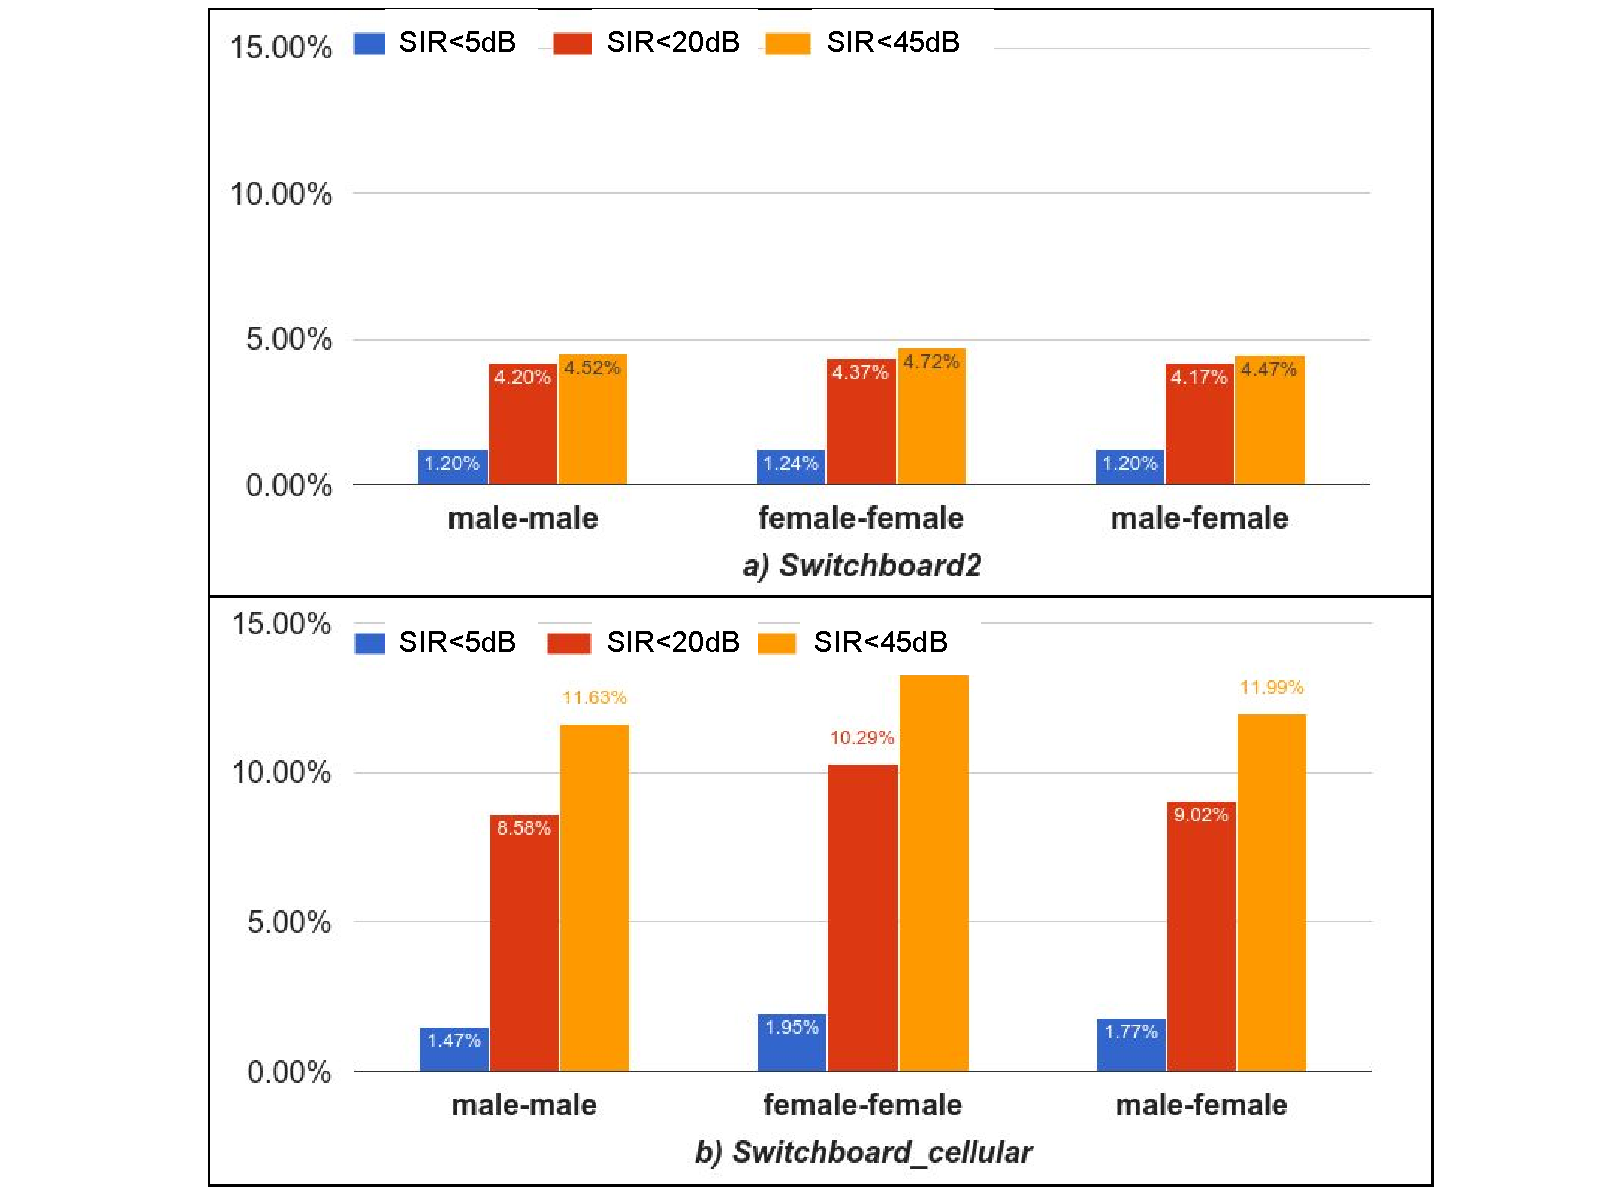
\includegraphics[height = 4in, width=0.8\textwidth]{figures/swb_overlap_percentage-crop}
	\vspace{-1mm}
	\caption{\it \small Percentage of overlaps to total speech in Switchboard2 and Switchboard cellular telephone conversations. Three SIR upper bounds are selected to label overlaps; 5dB, 20dB, 45dB. The higher the SIR upper bound, the stricter the overlap labels. Separate results are shown for male-male, male-female, and female-female conversations.}
	\label{fig:swb_overlap_percentage}
	\vspace{-3mm}
\end{figure*}


\begin{figure}[b!]
	\vspace{0mm}
	\centering
	\textbf{Overlap in meetings}\par\medskip
	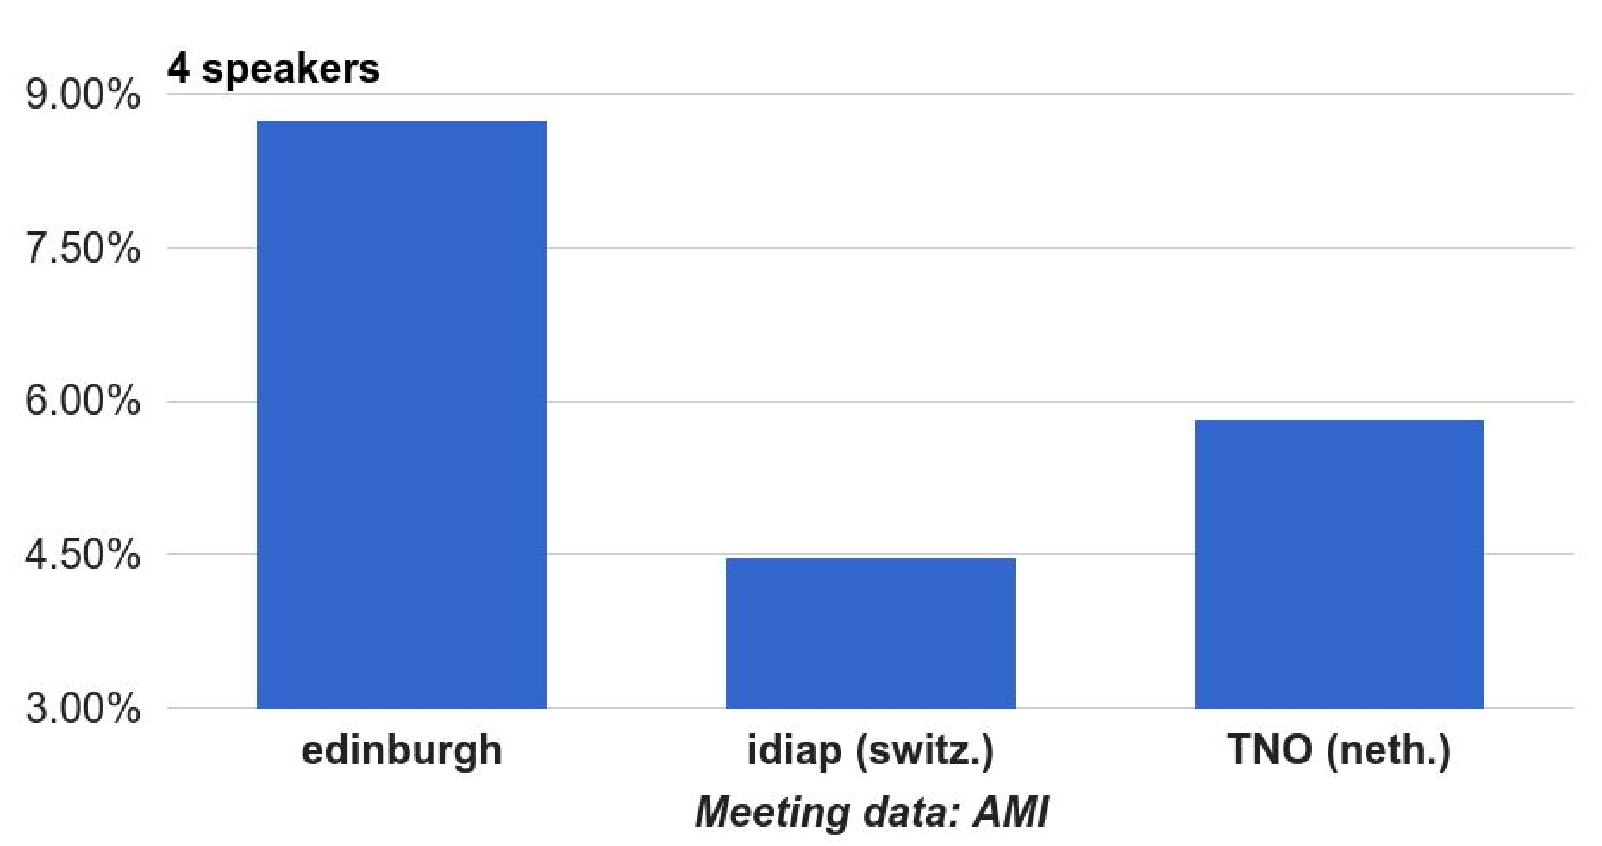
\includegraphics[height = 2.8in, width=0.5\textwidth]{figures/ami_overlap_percentage-crop}
	\vspace{-3mm}
	\caption{\it \small Percentage of overlaps to total speech in the AMI meeting corpus. All meetings used here have exactly 4 speakers. 
	The percentage of overlap is significantly higher here compared to Switchboard (compare with blue bars in Fig.~\ref{fig:swb_overlap_percentage}).}
	\label{fig:ami_overlap_percentage}
	\vspace{-3mm}
\end{figure}


To investigate the amount of overlap in conversational speech, two popular corpora are examined here: 
\begin{itemize}
	\item Switchboard2: a large collection of five minute telephone conversations involving several hundred speaker from across the United States.
	\item Switchboard Cellular: five-six minute telephone conversations on cellular phones.
	\item AMI meeting corpus: A dataset consisting of 100 hours of meeting recordings from several locations across Europe. 
\end{itemize}
For each session, the separate (almost interference-free) channels provided for each speaker are first segmented into speech and silence using an energy-based speech activity detection. 
Signal energies are required for each time-frame ($25msec window$), since signal-to-interference ratio (SIR) is used to define overlap. 

\begin{equation}
\label{eq:abs_sir}
SIR(n) = 10log_{10}(\frac{P_1(n)}{P_2(n)})
\end{equation}
where $P_1(n)$ is the per-frame energy of channel 1 and $P_2(n)$ corresponds to channel 2. $n$ represents frame indexes. 
Channels are mixed (per sample addition of the two signals) to create co-channel data. 
Instances at which both speakers are active are considered overlapped. 
Since the SIR value varies for different segments, we use a threshold on the SIR to label frames as overlapped. 
Segments with absolute SIR (i.e., $|SIR|$) lower than the threshold are considered overlapped.
The amount of overlap varies with the maximum allowable SIR (i.e., threshold) set by the evaluator. 
For instance, one might consider the mere presence of two speakers at the same time sufficient to label a segment as overlap, which is an indication of high SIR thresholds ($45dB$ in Fig.~\ref{fig:swb_overlap_percentage}). 
A more pragmatic view, however, is to choose an SIR small enough to preserve as much data possible. 
This way of preserving some overlapped segments is shared in many studies under the definition of usable speech~\cite{yantorno_report,smolenski_tut}. 
Lower SIR values, $(0-5) dB$, have a more significant impact on speaker verification, but to provide more insight, three SIR upper bounds have been used in Fig.~\ref{fig:swb_overlap_percentage}; $5$, $20$, $45dB$. 
We argue that any overlap up to $5dB$ should have noticeable impact on speaker verification. 
An upper bound of $45dB$ is also chosen, since the percentage of overlap is constant beyond $45dB$. 
It is shown in Fig.~\ref{fig:swb_overlap_percentage} that with a $5dB$ threshold, the percentage of overlap to total speech is below $2\%$. 
For the curios reader, we have provided overlap percentages for three groups of conversations: male-male, male-female, and female-female pairs. 
It is clear that for Switchboard gender does not play a role in dictating overlap percentage. 

For a broader perspective, we also analyze the AMI meeting corpus. 
The difference between meetings and phone conversations is in the number of speakers and face-to-face interaction. 
we speculate that number of speakers increases overlap while on the other hand the fact that all speakers are present in the same room (i.e., face-to-face interaction) limits the amount of overlap. 
Another difference is that SIR is not as well defined for meetings as it is for two-party phone-calls, since multiple parties may be active at the same time. 
In Fig.~\ref{fig:ami_overlap_percentage}, we assume at least two speakers should have a relative SIR of up to $5dB$. 
Any additional speaker is evaluated with respect to the primary speaker, but with a $20dB$ threshold. 
As Fig.~\ref{fig:ami_overlap_percentage} suggests, location also plays a significant role in overlap percentage. 
The authors refrain from speculating the impact of location, since it exceed the scope of this study. 

In text-independent speaker recognition, where we are interested in long-term acoustic characteristics, 4-5\% of overlapped speech in our data has little effect on speaker recognition accuracy. 
The point here is not to say that overlapped speech can be neglected in speaker recognition, but to clarify that speaker recognition in its most common form is more concerned with co-channel speech in general rather than {\it overlap} as it appears in everyday English conversations. 
In the more general case of co-channel speech interference, the presence of secondary speakers has a significant impact on speaker verification. 
We roughly estimate that in a two-party phone conversation, approximately $50\%$ of the data contains the unwanted secondary speaker (compare this with $2\%$ in Fig.~\ref{fig:swb_overlap_percentage}). 
Section~\ref{ssec:cch_in_trials} will investigate the effect of overlap and co-channel on speaker verification EER. 



\subsection{Co-channel Interference in Trials}
\label{ssec:cch_in_trials}
In this section, a series of speaker verification experiments are conducted on Switchboard2 to demonstrate the effect of using co-channel speech in enrollment and test data. 
We do not introduce these experiments as ``baseline'', since it is an unfair assessment to add co-channel interference to trials and expect PLDA to perform well. 
The purpose of this section is to show the increase in equal error rates as a result of co-channel speech. 
We also further emphasize the point made in Sect.~\ref{sec:cochannl_in_sid} by identifying the impact of overlap from co-channel interference on the EER. 

\begin{figure*}[t!]
	\vspace{-1mm}
	\centering
	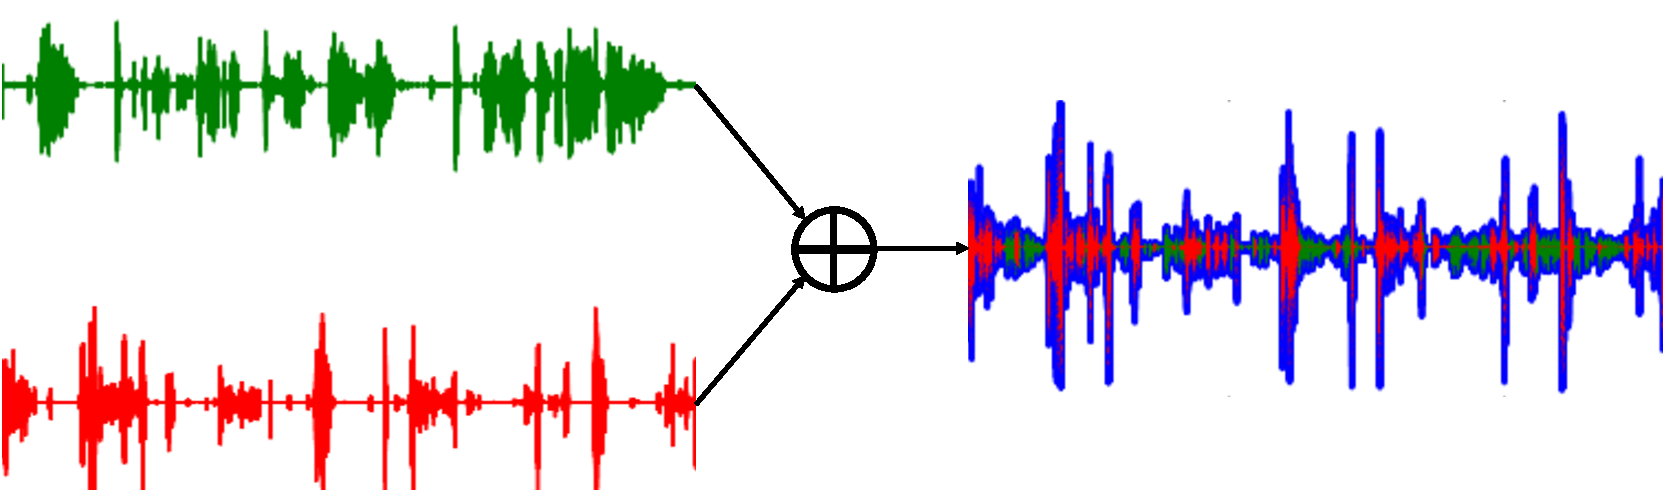
\includegraphics[height = 1.0in, width=0.45\textwidth]{figures/swb_cch_demo-crop}
	\vspace{-1mm}
	\caption{\it \small Mixing two channels of a Switchboard phonecall. The example here mixes the signals with 0dB SIR. Blue shows the resulting co-channel signal. Red and green each show one of the single-speaker signals.}
	\label{fig:mix_swb}
	\vspace{-1mm}
\end{figure*}

For these experiments, single-speaker data is used to estimate PLDA parameters (not co-channel data). 
Trials are evaluated at different levels of co-channel interference (i.e., SIR level). 
In each scenario, trial recordings are summed with their counterpart channel from the phone conversation to create co-channel data, as if speakers are speaking on a single channel (shown in Fig.~\ref{fig:mix_swb}). 
Speaker labels for trial recordings are generated based on the foreground speaker. 
In this context, foreground speaker refers to the speaker of interest. 
For example, in a $5dB$ co-channel session generated from Switchboard2 containing speakers {\bf X} and {\bf Y}, if {\bf X} were the foreground speaker, the average energy of {\bf X} would be $5dB$ higher than the average energy of {\bf Y}. 
%Therefore, $SIR_{trial}$ is defined slightly differently from here on after, compared to the per-sample absolute $SIR(n)$ in (\ref{eq:abs_sir}). 
%\begin{equation} 
%SIR_{trial} = 10log_{10}\Big(\frac{\frac{1}{T}\sum_t E_X(t)}{\frac{1}{T}\sum_t E_Y(t)}\Big), \hspace{30pt} t=1,...,N
%\end{equation}
%where $E_X(t)$ and $E_Y(t)$ are signal energies at frame $t$. 
Five SIR levels are chosen throughout experiments; $100dB$ (i.e., clean sessions), $20dB$, $10dB$, $5dB$, and $0dB$. 
In $0dB$ the average energy of the foreground and background data is equal. 
To avoid mismatch, the clean condition is also generated through the same procedure with an SIR of $100dB$ favoring the foreground speaker. 

A gender-independent universal background model (UBM) is created using 8kHz single-speaker NIST SRE data from 2004, 2005, and 2006 challenges~\cite{NIST04,NIST05,NIST06}. 
The UBM consists of $2048$ Gaussian mixtures representing a 39 dimensional feature space (13 dimensional MFCC plus $\Delta$ and $\Delta\Delta$). 
The same data from SRE 2004-6 is used to estimate a total variability (TV) matrix, which extracts $400$ dimensional i-vectors~\cite{Dehak_ivector}. 
The data used here to estimate PLDA parameters are single-speaker recordings from NIST SRE 2008~\cite{NIST08}. 
PLDA training data consists of approximately $11k$ single-speaker utterances from over $1300$ speakers. 
Trial data is developed from 2500 Switchboard2 recording sessions containing approximately $800$ speakers. 
Prior to feature extraction, trials are processed using comboSAD, an unsupervised speech activity detection~\cite{sadjadi2013unsupervised}. ComboSAD has previously shown to provide stable performance improvement in such speaker recognition tasks~\cite{hasan2013crss}. 

Figure~\ref{fig:cch_in_sid} shows speaker verification performance for the five SIR cases. 
As shown, EER for the clean condition is significantly lower than all the other SIR levels, even $20dB$. 
The sudden jump in EER shows the significance of co-channel interference. 

\begin{figure}[h!]
	\centering
	\textbf{Speaker recognition in co-channel}\par\medskip
	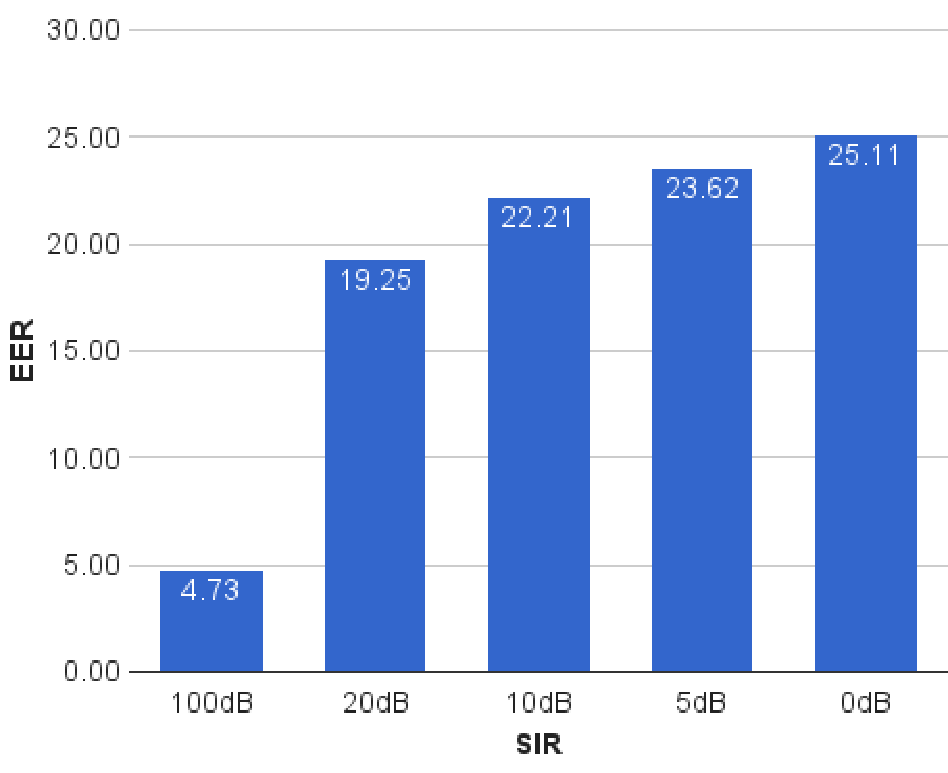
\includegraphics[height = 2.8in, width=0.5\textwidth]{figures/eer_vs_sir_swb2_baseline}
	\vspace{-2mm}
	\caption{\it \small Speaker verification performance with co-channel speech in switchboard trials. The i-vector/PLDA system uses a typical system configuration and is fully trained on single-speaker data. The purpose of this chart is to show the rapid increase in equal error rate (EER) as co-channel data is added to the trials. 100dB SIR represents clean (single-speaker) trials.}
	\label{fig:cch_in_sid}
	\vspace{-1mm}
\end{figure}

A second experiment is conducted to separate performance drop caused by overlap. To show this, all speech from the secondary speaker is dropped from the recordings, except for segments that overlap with the foreground speaker. 
This is accomplished by using voice activity detection (VAD) labels from the 100dB trials, while using $0dB$ audio data for the trials. 
Figure~\ref{fig:ovl_in_sid}, compares speaker verification under overlap with 0dB co-channel speech. 

\begin{figure}[h!]
	\vspace{-1mm}
	\centering
	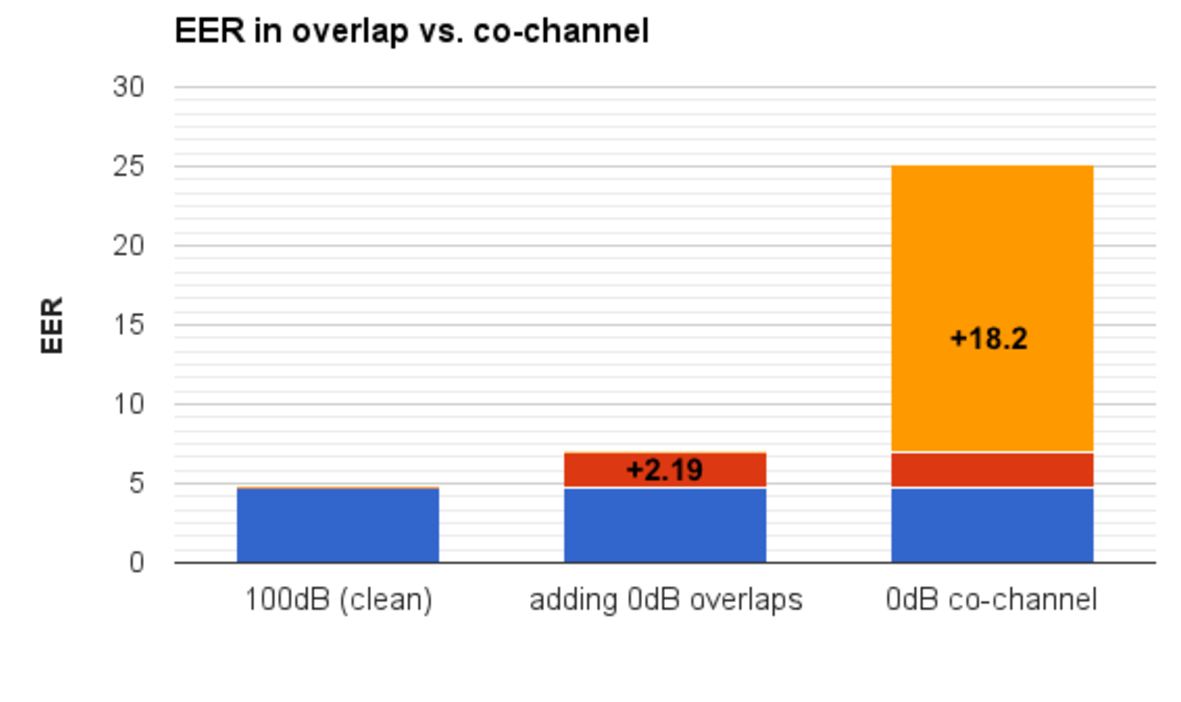
\includegraphics[height = 2.8in, width=0.5\textwidth]{figures/overlap_vs_cochannel_sid-crop}
	\vspace{-8mm}
	\caption{\it \small Comparing the effect of overlap in speaker verification with the more general case of co-channel. This study differentiates overlap from co-channel speech by considering overlaps to be segments during which both speakers are active. Co-channel refers to the more general case of two speakers in an audio stream, not necessarily overlapped (see Fig.~\ref{fig:cochannel_vs_overlap}). The chart shows that overlap plays a small part in the rise of EER compared to co-channel interference.}
	\label{fig:ovl_in_sid}
	\vspace{-1mm}
\end{figure}


\section{Motivation}
\label{sec:background}
Before presenting our proposed methods, it is essential to provide a brief overview of the chronological introduction and development of probabilistic linear discriminant analysis (PLDA) in speaker recognition. 
PLDA was initially proposed for face recognition in~\cite{prince_plda}. 
It was later adopted as a channel compensation step for speaker recognition using i-vectors~\cite{kenny2010bayesian}. 
A number of studies since then have presented different formulations for the factor loading paradigm most commonly known as PLDA. 
In this study, we are specifically interested in three formulations: 1) standard PLDA~\cite{kenny_plda}, 2) simplified PLDA~\cite{kenny_plda2,Daniel2011is}, and 3) the two-covariance model~\cite{brummer2010twocov}. 
The nomenclature used here is adopted from a recent study by Sizov et al.~\cite{sizov2014unifying} aimed at unifying the variations proposed for PLDA over the past decade. 


\subsection{Standard PLDA}
\label{ssec:standard_plda}
The general idea of probabilistic linear discriminant analysis is to find a subspace in the i-vector space that best represents speaker-specific components. 
The search for this subspace is based on a training dataset organized in a way that emphasizes differences between speakers as well as variations of each speaker across different recordings (aka sessions). 
The data organization comprises $n_i$ observation i-vectors for speaker $i$ from a set of development speakers, PLDA assumes the following linear factorization for each i-vector ${\bf m}_{ij}$: 

\begin{equation}
\label{eq:std_plda}
{\bf m}_{ij} = {\bf m}_g + {\bf V}{\bf y}_i+{\bf U}{\bf x}_{ij}+{\bf z}_{ij},  \hspace{30pt} j=1,...,n_i
\end{equation}
where $m_g$ represents the global i-vector mean. Speaker- and session-dependent latent variables, ${\bf y}_i$ and ${\bf x}_{ij}$, take a standard normal distribution, $\mathcal{N}({\bf 0},{\bf I})$. ${\bf V}$ and ${\bf U}$ are typically tall matrices representing eigenvoice and eigenchannel subspaces, respectively. Eigenvoice refers to the collection of factor loadings (represented in ${\bf V}$) that construct the speaker-dependent subspace. Eigenchannel refers to the session-dependent subspace. 
In addition to the eigenchannel subspace a session-dependent and normally distributed slack variable, ${\bf z}_{ij}$, is included to express session variabilities. In (\ref{eq:std_plda}), $z_{ij}$ takes a diagonal covariance matrix, $\mathcal{N}({\bf 0},{\bf \Sigma_d})$,~\cite{kenny_plda,prince_plda}. 
PLDA predicts model parameters, $({\bf V},{\bf U},{\bf \Sigma_d})$, using the expectation-maximization (EM) algorithm~\cite{prince_plda}. 
After estimating subscpace components using background development data, trial i-vectors are reduced to the same speaker-dependent subspace using PLDA and scored through a hypothesis testing procedure (see~\cite{prince_plda} for details). 
The hypothesis testing stage estimates the likelihood ratio of whether two trial i-vectors (train and test) belong to the same speaker, or if they belong to two different speakers. 

\subsection{Simplified PLDA}
\label{ssec:simplified_plda}
The second formulation reduces complexity in (\ref{eq:std_plda}) using the fact that session-dependent latent variables (${\bf x}_{ij}$ in (\ref{eq:std_plda})) are not directly used in the scoring process. 
Therefore, as long as models are able to effectively estimate the eigenvoice subspace, channel-dependent components (essentially all non-speaker dimensionality) are redundant. 
With this in mind, the second term in (\ref{eq:std_plda}) is removed in simplified PLDA and all channel information is captured in the slack variable. 
The slack variable in this case is assumed to have a full covariance matrix.

\begin{equation}
\label{eq:simple_plda}
{\bf m}_{ij} = {\bf m}_g + {\bf V}{\bf y}_i+{\bf z}^f_{ij}.  \hspace{30pt} j=1,...,n_i
\end{equation}
The use of a full covariance matrix in the slack variable can be interpreted as combining the diagonal slack covariance in (\ref{eq:std_plda}) with the eigenchannel subspace projection ${\bf UU}^T$~\cite{sizov2014unifying}.
We consider this formulation our baseline. 

\subsection{PLDA as an extension to LDA}
\label{sec:twocov}
The last interpretation, called the two-covariance model~\cite{sizov2014unifying}, is a probabilistic extension to linear discriminant analysis (LDA). 
The two-covariance model describes the i-vector space in terms of between- and within-speaker covariances, as does LDA. 
It is well known that LDA models feature spaces as a mixture of Gaussians, in which each mixture has the same covariance, ${\bf \Phi_w}$. 
Gaussian mixtures represent within-class (i.e., session) variability, therefore ${\bf \Phi_w}$ is referred to as the within-class covariance matrix. 
LDA is commonly used to find the optimal discriminating subspace of a given set of training speakers, relative to their within-speaker variation~\cite{ioffePLDA2006}. 
The problem, however, is that the aforementioned subspace is only optimal for the given training speakers. 
What LDA fails to provide is a continuous (or in this context, stochastic) representation of each mixture's centroid\footnote{In i-vectors, centroids are known to correspond to speakers. In other words, each centroid represents a speaker.}. 
Therefore, centroids are considered deterministic in LDA. 
When a new speaker is introduced, the resulting projection of LDA is not necessarily reliable. 
PLDA provides a stochastic representation of class centroids using a between-class covariance matrix, ${\bf \Phi_b}$~\cite{ioffePLDA2006}. 
The centroid distribution assumes a continuous centroid subspace, which acknowledges the possibility of unseen speakers. 
PLDA can therefore be defined as a combination of two distributions; 
\begin{enumerate}
	\item the distribution of i-vectors in each class representing a certain speaker, which is a Gaussian with mean $m_c$, mean of a speaker's i-vectors, and covariance ${\bf \Phi_w}$. $c$ here represents the class label, or speaker identity. Therefore, the probability of an i-vector, $m$, given that it comes from class $c$ is:
	\begin{equation}
	\label{eq:within_spk_dist}
	{\bf m} \sim \mathcal{N} ({\bf m}_c,{\bf \Phi_w} | c),
	\end{equation}
	\item the class centroid distribution, also assumed Gaussian:
	\begin{equation}
	\label{eq:between_spk_dist}
	{\bf m}_c \sim \mathcal{N} ({\bf m}_g,{\bf \Phi_b}),
	\end{equation}
	where ${\bf m}_g$ is the global mean of all class centroids (assumed to be equal to the global mean of all i-vectors) and ${\bf \Phi_b}$ is the between-speaker covariance matrix. 
\end{enumerate}

Defining channel variability as a function of speaker variation helps PLDA model unseen speakers (i.e., speakers that are not present in the development set). 
As opposed to LDA, which is incapable of offering optimal solutions to speakers that are absent from the training set~\cite{ioffePLDA2006}. 
The interpretation in this section, provides a perspective which we will use in our proposed method (Sect.~\ref{sec:cch_plda}) to investigate adding co-channel interference as a contributor to within-class variability. 
Using a transformation matrix (${\bf V}$), equations (\ref{eq:within_spk_dist}) and (\ref{eq:between_spk_dist}) can be translated to (\ref{eq:simple_plda})~\cite{sizov2014unifying} in which the within- and between-covariances are diagonalized~\cite{ioffePLDA2006}. 


\section{Proposed method: mixed PLDA}
\label{ssec:plda_data_prep}
The search for eigenvoice and eigenchannel subspaces involves a careful selection of development data. 
The idea in data preparation for PLDA is to provide sufficient channel diversity for each speaker to model within-speaker variations, while maintaining high speaker counts to model between-speaker variability. 
Channel and speaker variation introduced in the development data are directly translated into within- and between-speaker covariances, respectively. Said covariances are used to estimate PLDA parameters, (\ref{eq:std_plda}) and (\ref{eq:simple_plda})~\cite{sizov2014unifying}. 
The data-driven perspective towards channel compensation using PLDA has inspired a number of studies to address other types of variability through the same data selection procedure, where instead of channel diversity, one could generate a development set with age~\cite{kelly2013} or language diversity~\cite{misra2014languagemismatch} (in the case of multi-lingual speakers). 
Therefore, our first approach is to investigate co-channel speaker recognition performance when background PLDA data contains co-channel speech recordings. 

Co-channel recordings for each speaker are obtained from separate conversations. In these conversations, it is important to maintain diversity in secondary (aka interfering) speakers; since without sufficient secondary speaker diversity, the PLDA model will train to both primary and secondary speakers. 
Figure~\ref{fig:mixedPLDA_diagram} is a diagram of how the PLDA data is arranged in this approach, which we call ``mixed PLDA''. 
Mixed PLDA introduces speaker interference in the background development data using co-channel mixtures to implicitly train the PLDA model to recognize speaker interference as session variability. 


\begin{figure}[t!]
	\centering
	\vspace{0mm}
	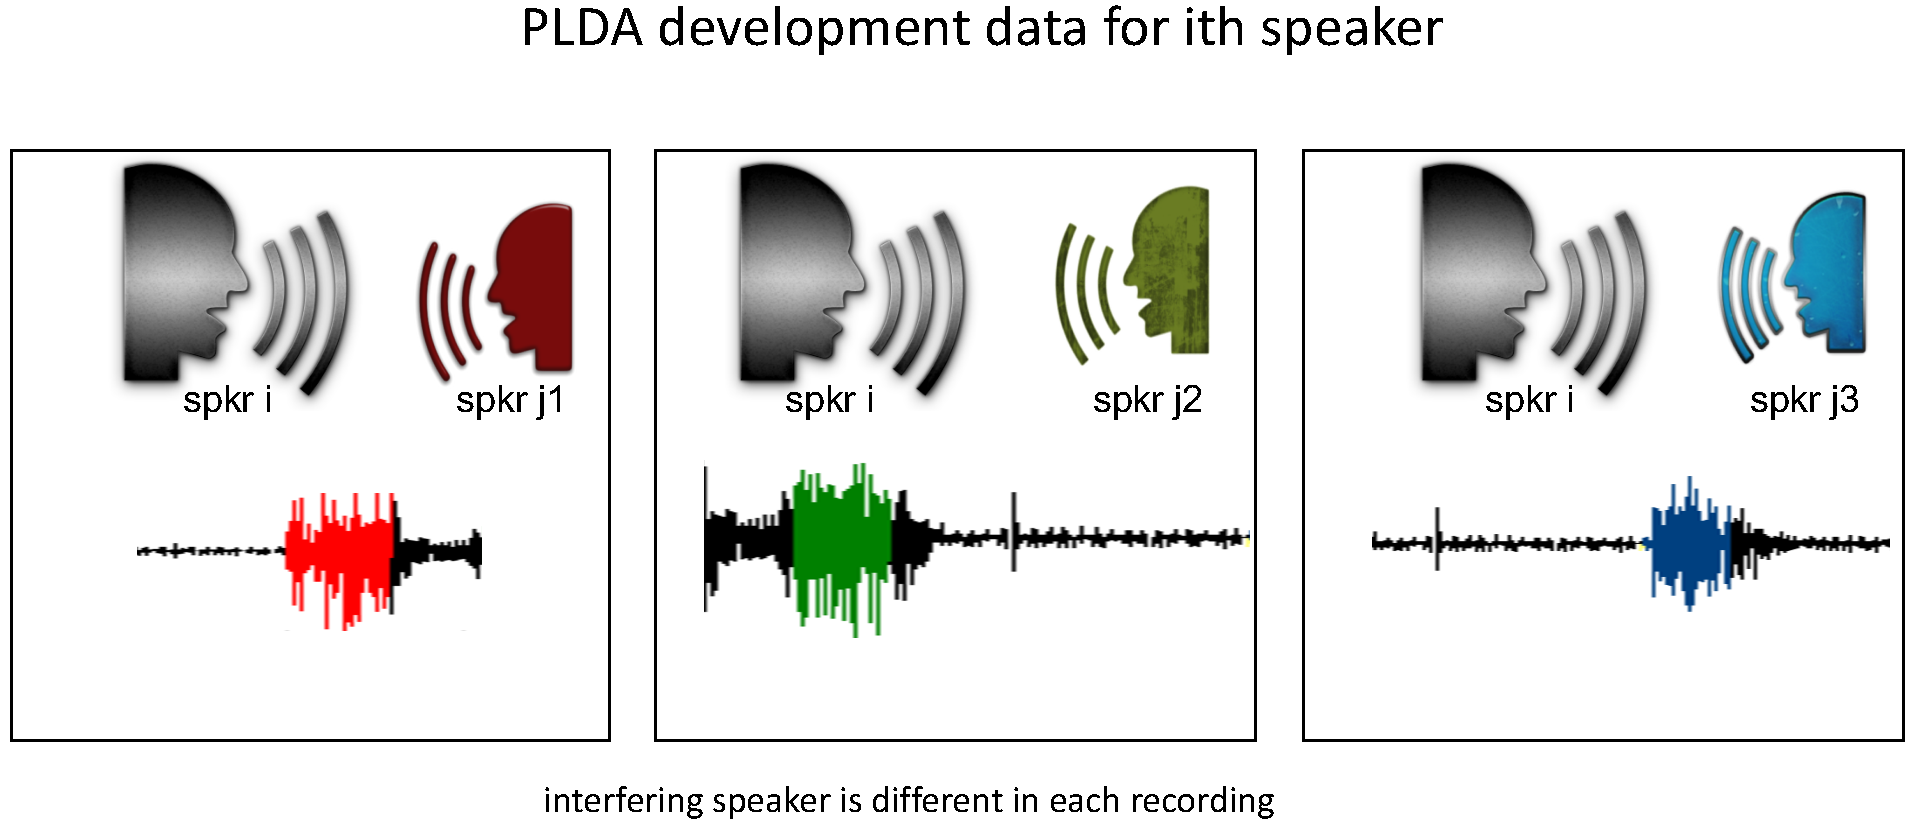
\includegraphics[width=0.6\textwidth, height=2in]{figures/mixedPLDA_slide-crop}
	\vspace{0mm}
	\caption{\it \small Creating development data for co-channel aware PLDA. the mixed PLDA approach uses co-channel data for each speaker in the background model. Recordings for the $i^{th}$ speaker consists of co-channel sessions with different speakers.}
	\label{fig:mixedPLDA_diagram}
	\vspace{-3mm}
\end{figure}

Mixed PLDA describes the use of co-channel background data in simplified PDLA, (\ref{eq:simple_plda}). 
This will be used as a baseline to provide fair comparison with our proposed PLDA formulation described in the next section. 

\subsection{Co-channel Interference in Trials with mixedPLDA} 
\label{sssec:mixedplda_exp}

Now that we have introduced {\it mixed PLDA}, we evaluate its performance by adding co-channel data to the PLDA training set. 
There are a number of ways co-channel data can be inserted, particularly in the choice of SIR. 
We investigate three cases in our experiments: 
\begin{itemize}
	\item $0dB$: All co-channel data used to train PLDA is 0dB. 
	\item $(0,100)dB$: Half of the data is clean and the other half is $0dB$. 
	\item $(0,5,10,20,100)$: co-channel files are uniformly selected from one of these five SIR values. 
\end{itemize}

Table~\ref{tbl:mixed_plda} shows that mixed PLDA with half $0dB$ and half $100dB$ co-channel training data for PLDA causes the least damage in the clean condition (a.k.a $100dB$), from $4.73$ to $5.22$. Mixed PLDA ($0$,$100dB$) also reduces error rates the most. 
Minimum detection cost functions (minDCF) is calculated over the operating point ($C_{fa}=10, C_{miss}=1, prior = 0.001$). 
These observation are consistent with those reported in~\cite{shokouhi2015probabilistic}. 

\begin{table*}[b!]
	\small
	\centering
	\resizebox{\textwidth}{!}
	{
		\begin{tabular}{|l|c|c|c|c|c|c|c|c|c|c|c|}
		\hline
		\multirow{2}{*}{SIR (dB)} & \multicolumn{3}{c|}{mixed PLDA (0dB)}          & \multicolumn{3}{c|}{mixed PLDA (0,5,10,20,100dB)}  & \multicolumn{3}{c|}{mixed PLDA (0,100dB)}       & \multicolumn{2}{l|}{simplified PLDA} \\ \cline{2-12} 
		& \multicolumn{2}{r|}{EER (\%)} & minDCF         & \multicolumn{2}{c|}{EER (\%)} & minDCF             & \multicolumn{2}{c|}{EER (\%)} & minDCF          & EER(\%)           & minDCF           \\ \hline
		100                       & \multicolumn{2}{c|}{7.48}     & 0.587          & \multicolumn{2}{c|}{5.71}     & 0.809              & \multicolumn{2}{c|}{\bf 5.22}     & 0.472           & 4.73              & 0.407            \\ \hline
		20                        & \multicolumn{2}{c|}{19.75}    & 0.897          & \multicolumn{2}{c|}{17.49}    & 0.865              & \multicolumn{2}{c|}{\bf 17.14}    & 0.872           & 19.25             & 0.909            \\ \hline
		10                        & \multicolumn{2}{c|}{21.79}    & 0.941          & \multicolumn{2}{c|}{20.24}    & 0.923              & \multicolumn{2}{c|}{\bf 19.82}    & 0.918           & 22.21             & 0.944            \\ \hline
		5                         & \multicolumn{2}{c|}{23.20}    & 0.960          & \multicolumn{2}{c|}{21.86}    & 0.948              & \multicolumn{2}{c|}{\bf 21.02}    & 0.940           & 23.62             & 0.967            \\ \hline
		0                         & \multicolumn{2}{c|}{24.61}    & 0.976          & \multicolumn{2}{c|}{23.13}    & 0.971              & \multicolumn{2}{c|}{\bf 22.43}    & 0.963           & 25.11             & 0.985            \\ \hline
	\end{tabular}
	}
	\caption{Mixed PLDA: PLDA performance when co-channel interference is introduced as session variation, without changing the original PLDA formulation. The EER for simplified PLDA is presented in the last column for comparison. }
	\label{tbl:mixed_plda}
\end{table*}

It is interesting that the best performance is obtained with a 50-50 split of co-channel and clean data in the PLDA training set. 
At this point I do not have a clear explanation of why {\it mixed PLDA} ($0,100dB$) is superior to ($0dB$) or ($0,5,10,20,100dB$). 

\section{Proposed method: dual eigenvoice PLDA}
\label{sec:dualev_plda}

The approach in {\it mixed PLDA} relies on the ability of PLDA that compensates channel mismatch. 
PLDA recognizes the variabilities observed across different recordings for a given speaker and removes them from the speaker subspace (aka the eigenvoice factors in ${\bf V}$). 
Therefore, {\it mixed PLDA} treats interfering speech as channel mismatch. 
This is accomplished by adding co-channel i-vectors to the PLDA background data and leaving it to the PLDA model estimation process to recognize interfering speech and remove its effects in the speaker subspace. 
However, interfering speech is not effectively picked up by neither the eigenchannel matrix (in case of the standard PLDA in~(\ref{eq:std_plda})) nor the slack variable, in (\ref{eq:simple_plda}). 
We address this by introducing our second approach which is to add a speaker dependent term intended to model interfering speech. Since the second term also corresponds to speaker identities, it should as well be represented by the speaker subspace. 
We call this approach {\it dual eigenvoice PLDA}, for which the PLDA factorization is: 

\begin{equation}
\label{eq:cchplda}
{\bf m}_{ij} = {\bf V}{\bf y}_i+{\bf V}^\prime {\bf w}_{ij}+{\bf z}_{ij}.
\end{equation}
Since the model still needs to represent channel variabilities, we keep ${\bf z}_{ij}$ as a full covariance normal distributed vector. 
${\bf V}^\prime$ represents the speaker dependent subspace, as does ${\bf V}$, with the difference that one is a rotation of the other with an unknown rotation factor. 
${\bf w}_{ij}$ is the latent variable which corresponds to the interfering speaker. 
There are a few reasons that prevent us from directly using ${\bf V}$ as factor loadings for the interfering components in~(\ref{eq:cchplda}), one being that as part of the degrees of freedom in the PLDA solution, the eigenvoice matrix can only be determined up to an unknown rotation matrix~\cite{sizov2014unifying} (similarly for ${\bf V}^\prime$). 
Equation (\ref{eq:cchplda}) uses different notation for the second eigenvoice matrix to remind us of this limitation. 
This prevents directly using ${\bf V}$ to represent the interfering speaker term. However, since we know that ${\bf V}$ and ${\bf V}^\prime$ must be related by a rotation matrix, we can use this knowledge to simultaneously update ${\bf V}$ and ${\bf V}^\prime$ in the EM iterations. 

As discussed, the relation between ${\bf V}$ and ${\bf V}^\prime$ is characterized by an unknown rotation matrix, ${\bf R}$:

\begin{equation}
{\bf V} = {\bf RV}^\prime.
\end{equation}
A reasonable ${\bf R}$ can be estimated via singular value decomposition (SVD) by considering the columns of ${\bf V}$ and ${\bf V}^\prime$ as data points in the speaker dependent subspace. The rotation matrix is derived from the cross-variance between ${\bf V}$ and ${\bf V}^\prime$ basis functions, ${\bf S}$:

\begin{equation}
{\bf S} = {\sum\limits_{i=1}^{N_V}\tilde{{v}_i}\tilde{{v}^\prime_i}^T},
\end{equation}
where $\tilde{v_i}$ is $v_i$ are the eigenvoice basis vectors centered at the origin and $N_V$ is the number of columns in ${\bf V}$ (and/or ${\bf V}^\prime$, since both have the same dimensions). The rotation matrix is defined as below:

\begin{equation}
{\bf R} = {\bf S}_{row}{\bf S}_{col}^T,
\end{equation}
where $S_{col}$ and $S_{row}$ are the column and row spaces of ${\bf S}$ obtained from SVD:

\begin{equation}
{\bf S} = {\bf S}_{col}{\bf \Lambda}{\bf S}_{row}^T.
\end{equation}

The rotation matrix is used in each iteration of the EM algorithm to update the matrix ${\bf V}^\prime$ and align it with ${\bf V}$, 

\begin{equation}
{\bf V}^\prime \leftarrow {\bf RV^\prime}. 
\end{equation}

Updating ${\bf V}^\prime$ before estimating the statistical statistics of latent variables, $y_{i}$ and $w_{ij}$, removes the redundancy in the second term of equation~(\ref{eq:cchplda}) by replacing the eigenvoice matrix ${\bf V}^\prime$ with information obtained from the basis vectors in ${\bf V}$. Since both factors in~(\ref{eq:cchplda}) are guided towards representing the speaker space, the overall system achieves a better estimate of ${\bf V}$ and Consequently more accurate estimates for latent variable statistics. 

\subsection{Co-channel Interference in Trials with dual eigenvoice PLDA} 
\label{ssec:dualevplda_exp}

\begin{figure*}[b!]
	\centering
	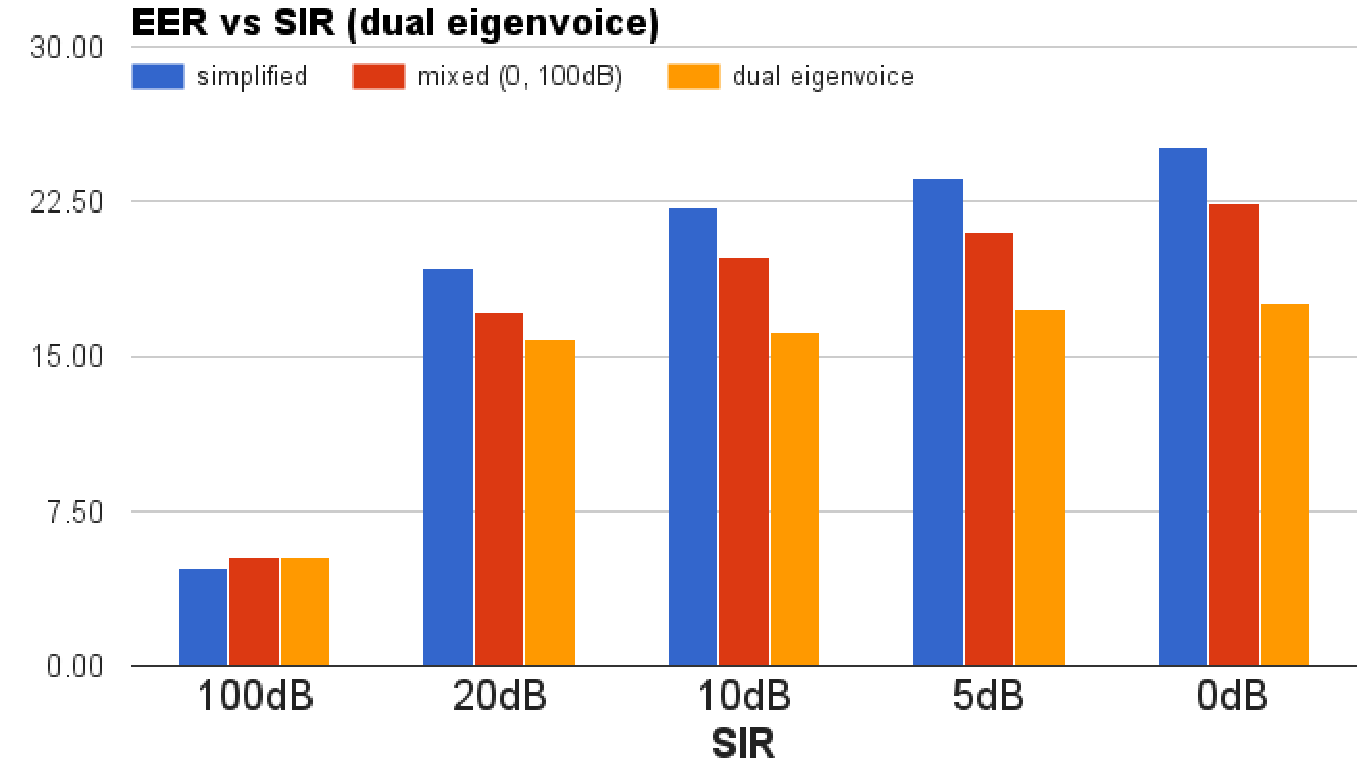
\includegraphics[height = 2.5in, width=0.5\textwidth]{figures/eer_vs_sir_dualeigenvoice}
	\vspace{-2mm}
	\caption{\it \small Comparing {\it dual eigenvoice PLDA}(yellow) with {\it mixed PLDA} (red) and {\it simplified PLDA} (blue). A steady improvement over {\it mixed PLDA} is observed across co-channel conditions. }
	\label{fig:eer_dualeigenvoice}
	\vspace{-1mm}
\end{figure*}

As described in Sect.~\ref{sec:dualev_plda}, {\it dual eigenvoice PLDA} attempts to model a linear factorization of the i-vectors into a target speaker and an interfering speaker component (see Eq.~(\ref{eq:cchplda})). 
PLDA is able to distinguish the target speaker using the several recordings available for each speaker. 
The key difference between this method and {\it mixed PLDA} is that the system is forced to use a similar subspace to model the interfering speaker. 
Figure~\ref{fig:swb_sid_results} shows the EER for different amounts of co-channel interference introduced to the trials. 

Considering that {\it simplified PLDA} does not claim robustness towards co-channel interference, it shows little resistance as trial SIR values increase. 
Since {\it mixed PLDA} has some observation of the co-channel condition, it reduces the EER for at least 1\% across all SIR conditions, as was shown in Sect.~\ref{sssec:mixedplda_exp}. {\it Dual eigenvoice PLDA}, further improves the performance and obtains 2.5-3.5\% drop in EER in all conditions. EER variations are significantly different for {\it dual eigenvoice PLDA} model compared to the other two systems. 
Figure~\ref{fig:eer_dualeigenvoice} shows that the clean-to-$0dB$ EER range for {\it mixed PLDA} is more than twice as much as {\it dual eigenvoice PLDA}. 



\subsection{convergence of Dual eigenvoice PLDA}
\label{ssec:convergence_dualevplda}
An interesting observation was made while developing {\it dual eigenvoice PLDA} regarding the convergence of model parameters, specifically the second eigenvoice matrix. 
Later, with some more investigation and feedback from experts in the field, I realized a significant flaw in the proposed formulation. 
This section provides a brief description of the issue with {\it dual eigenvoice PLDA}. 

The claim in {\it dual eigenvoice PLDA} is that the first eigenvoice matrix in (\ref{eq:simple_plda}) contains factor loadings corresponding to the primary speaker and the second eigenvoice matrix (i.e., ${\bf V}^\prime$) is for secondary speakers. 
We also chose a full-covariance slack variable, ${\bf z}$. 
The problem here arises from the full-covariance slack variable. 


\section{Proposed method: Co-channel Aware PLDA}
\label{sec:cch_plda}
This section describes our proposed approaches, which are modifications to the PLDA formulation (Sect.~\ref{sec:background}) that allow modeling speaker interference in ways that are more appropriate for co-channel speech. 
Previously, in~\cite{shokouhi2015probabilistic}, we proposed a modified PLDA formulation to remove secondary speaker interference from the latent variable subspace. 
This study uses different methods based on the two-covariance interpretation (described in Sect.~\ref{sec:twocov}). 
%Part of the reason for our departure from the co-channel PLDA formulation proposed in~\cite{shokouhi2015probabilistic} was our inability to justify certain behavior in the model. 
Our method, which we call {\it co-channel aware PLDA} (caPLDA), uses the dual distribution definition of (\ref{eq:within_spk_dist}) and (\ref{eq:between_spk_dist}) to model a co-channel i-vector. 

As mentioned before, caPLDA adopts the two-covariance interpretation of PLDA briefly described in (\ref{eq:within_spk_dist}) and (\ref{eq:between_spk_dist}). 
The i-vectors of a given class can be modeled as a normally distributed vector with a mean pertaining to the class to which it belongs and a covariance matrix representing within class variability, (\ref{eq:within_spk_dist}). 
Typically, within-class variability is meant to model channel variation across sessions. 
In the case of co-channel speech, in addition to channel variability, one must consider the variability caused by interfering speakers. 
We will see in Sect.~\ref{ssec:cch_in_trials} that speaker interference has a dramatic impact on error rates. Much more compared to channel variation in a dataset such as Switchboard. 
It is therefore reasonable to prioritize co-channel interference over channel mismatch. 

In Sect.~\ref{ssec:plda_data_prep}, we proposed capturing speaker interference in the same manner that channel variation is captured by PLDA. 
Although some improvement is attainable, we expect that the original PLDA formulation, (\ref{eq:simple_plda}), is not capable of fully capturing speaker interference; partly due to the similarity between speaker-dependent latent variables and the cross-session variations that exist in co-channel interference. 

We propose that in order to improve performance, information can be shared from the between-speaker covariance to within-class covariances. 
For an i-vector with speaker $A$ as the foreground speaker and some speaker $X$ as secondary speaker, PLDA assumes a normal distribution $\mathcal{N} ({\bf m}_A,{\bf \Phi} | A)$. 
While (\ref{eq:within_spk_dist}), considers ${\bf \Phi}$ to be a unique within-class covariance matrix for all speakers in the i-vector space (i.e., $\Phi_w$), we argue that an additional component is required to model within speaker variations in the case of co-channel i-vectors. 
The additional component contributing to within-class covariance is of the same nature of the between-class covariance. 
Therefore, one can assume that ${\bf \Phi}$ is a function of both ${\bf \Phi}_w$ and ${\bf \Phi}_b$, $ \mathcal{F} ({\bf \Phi}_w,{\bf \Phi}_b)$. 
Our suggested structure for $ \mathcal{F} (.,.)$ is a linear combination of the two covariance matrices: 

\begin{equation}
\label{eq:complex_phiw}
\Phi = \mathcal{F} (\Phi_w,\Phi_b) = 
\alpha_w\Phi_w + \alpha_b\Phi_b
\end{equation}
where $\alpha_w$ and $\alpha_b$ are functions of the signal-to-interference ratio between the foreground and background speaker. 

Sections~\ref{ssec:alpha_w_0}~and~\ref{ssec:caplda_exp} visits different possibilities of $(\alpha_w, \alpha_b)$. But first, we find it useful to focus on a special case, which is to assume session variability should be of the exact same type as speaker variability in the case of co-channel i-vectors. 
This special case assumes equal within- and between-speaker covariances. 

\subsection{Equal within- and between-speaker covariances ($\alpha_w = 0$)}
\label{ssec:alpha_w_0}
In~\cite{ioffePLDA2006}, PLDA model parameters are learned by maximizing the likelihood of observation i-vectors provided for each speaker (i.e., class). 
The likelihood is calculated by assuming the i-vectors are conditionally independent given the speaker. 
In this case, the probability of i-vectors $m^1, m^2, ..., m^n$ regardless of the speaker they were generated from, represented by $y$, is:

\begin{equation}
\mathcal{P}(m^1 m^2 ... m^n) = \int \mathcal{P}(y) \mathcal{P}(m^1 | y) \mathcal{P}(m^2 | y) ... \mathcal{P}(m^n | y) dy,
\end{equation}
Replacing the probabilities using (\ref{eq:within_spk_dist}) and (\ref{eq:between_spk_dist}), the log-likelihood of $\mathcal{P}(m^1 m^2 ... m^n)$ is: 


\begin{equation}
\label{eq:llk_twocov}
\begin{split}
\mathcal{L}(m^1 m^2 ... m^n) = -\frac{c}{2}(ln | {\bf \Phi}_b + \frac{1}{n}{\bf \Phi}_w | + tr(({\bf \Phi}_b + \frac{1}{n}{\bf \Phi}_w)^{-1}S_b) \\+ (n-1)ln|{\bf \Phi}_w| + ntr({\bf \Phi}_w^{-1}S_w)),
\end{split}
\end{equation}
where $S_b$ and $S_w$ are the between-speaker and within-speaker scatter matrices calculated from the training i-vectors. $c$ is a normalizing constant. 
The log-likelihood is maximized using (\ref{eq:llk_twocov}), resulting in expectation-maximization (EM) steps that estimate values for ${\bf \Phi}_w$ and ${\bf \Phi}_b$. 
If we ignore channel variability across sessions and assume that the only source of variation across different sessions is between-speaker variability, the probabilities $\mathcal{P} (x_i | y)$ change from $\mathcal{N} (y,\Phi_w)$ to: 

\begin{equation}
\mathcal{P} (x_i|y) = \mathcal{N} (y,\Phi_b).
\end{equation}

The assumption here is that within-session variation is similar to between-speaker variations (i.e., ${\bf \Phi}_b$). 
This assumption is equivalent to setting $\alpha_w$ to $0$ and $\alpha_b$ to $1$ in (\ref{eq:complex_phiw}). 
The upside of setting ${\bf \Phi}$ to ${\bf \Phi}_b$ is twofold: 1) it increases the accuracy of estimating ${\bf \Phi}_b$, since in this scenario within-speaker differences can also be used to calculate ${\bf \Phi}_b$. 2) The maximum likelihood problem in (\ref{eq:llk_twocov}) is reduced to:

\begin{equation}
\label{eq:llk_onecov}
\begin{split}
\mathcal{L}(m^1 m^2 ... m^n) = -\frac{c}{2}(nln | {\bf \Phi}_b | + ln(\frac{n+1}{n})+ \frac{n}{n+1}tr({\bf \Phi}_b^{-1}S_b) \\+ ntr({\bf \Phi}_b^{-1}S_b)),
\end{split}
\end{equation}
which is simpler to maximize. In fact, when all speakers have the same number of training i-vectors ($n$), the solution is to set $\Phi_b$ to $S_b$. 



\subsection{Co-channel Interference in Trials with caPLDA}
\label{ssec:caplda_exp}
Finally, we would like to analyze the potential gain in using alternative PLDA formulations described in Sect.~\ref{sec:cch_plda}. 
Instead of a grid-search of all possible $(\alpha_w,\alpha_b)$ inputs, only a selection of are presented here that we think provide most useful insight. 

Figure~\ref{fig:alpha_w_is_1}, shows the case in which $\alpha_w$ is set to $1$ and $alpha_b$ varies from $0$ to $1$. 
The EER values are almost unequivocally lower than their counterparts presented in Tab.~\ref{tbl:mixed_plda}, despite the fact that they do not use mixed PLDA training data. 
In other words, the EER values calculated in Fig.~\ref{fig:alpha_w_is_1} show performance using clean ($100dB$) PLDA training. 
The bottom line (blue) shows EER for clean trials. 
As expected, EER values slightly increase in the clean condition, when the original PLDA formulation is modified. 
However, in lower SIR conditions ($20-0dB$), more performance gain is observed as $alpha_b$ approaches $0.1$. 

\begin{figure*}[h!]
	\centering
	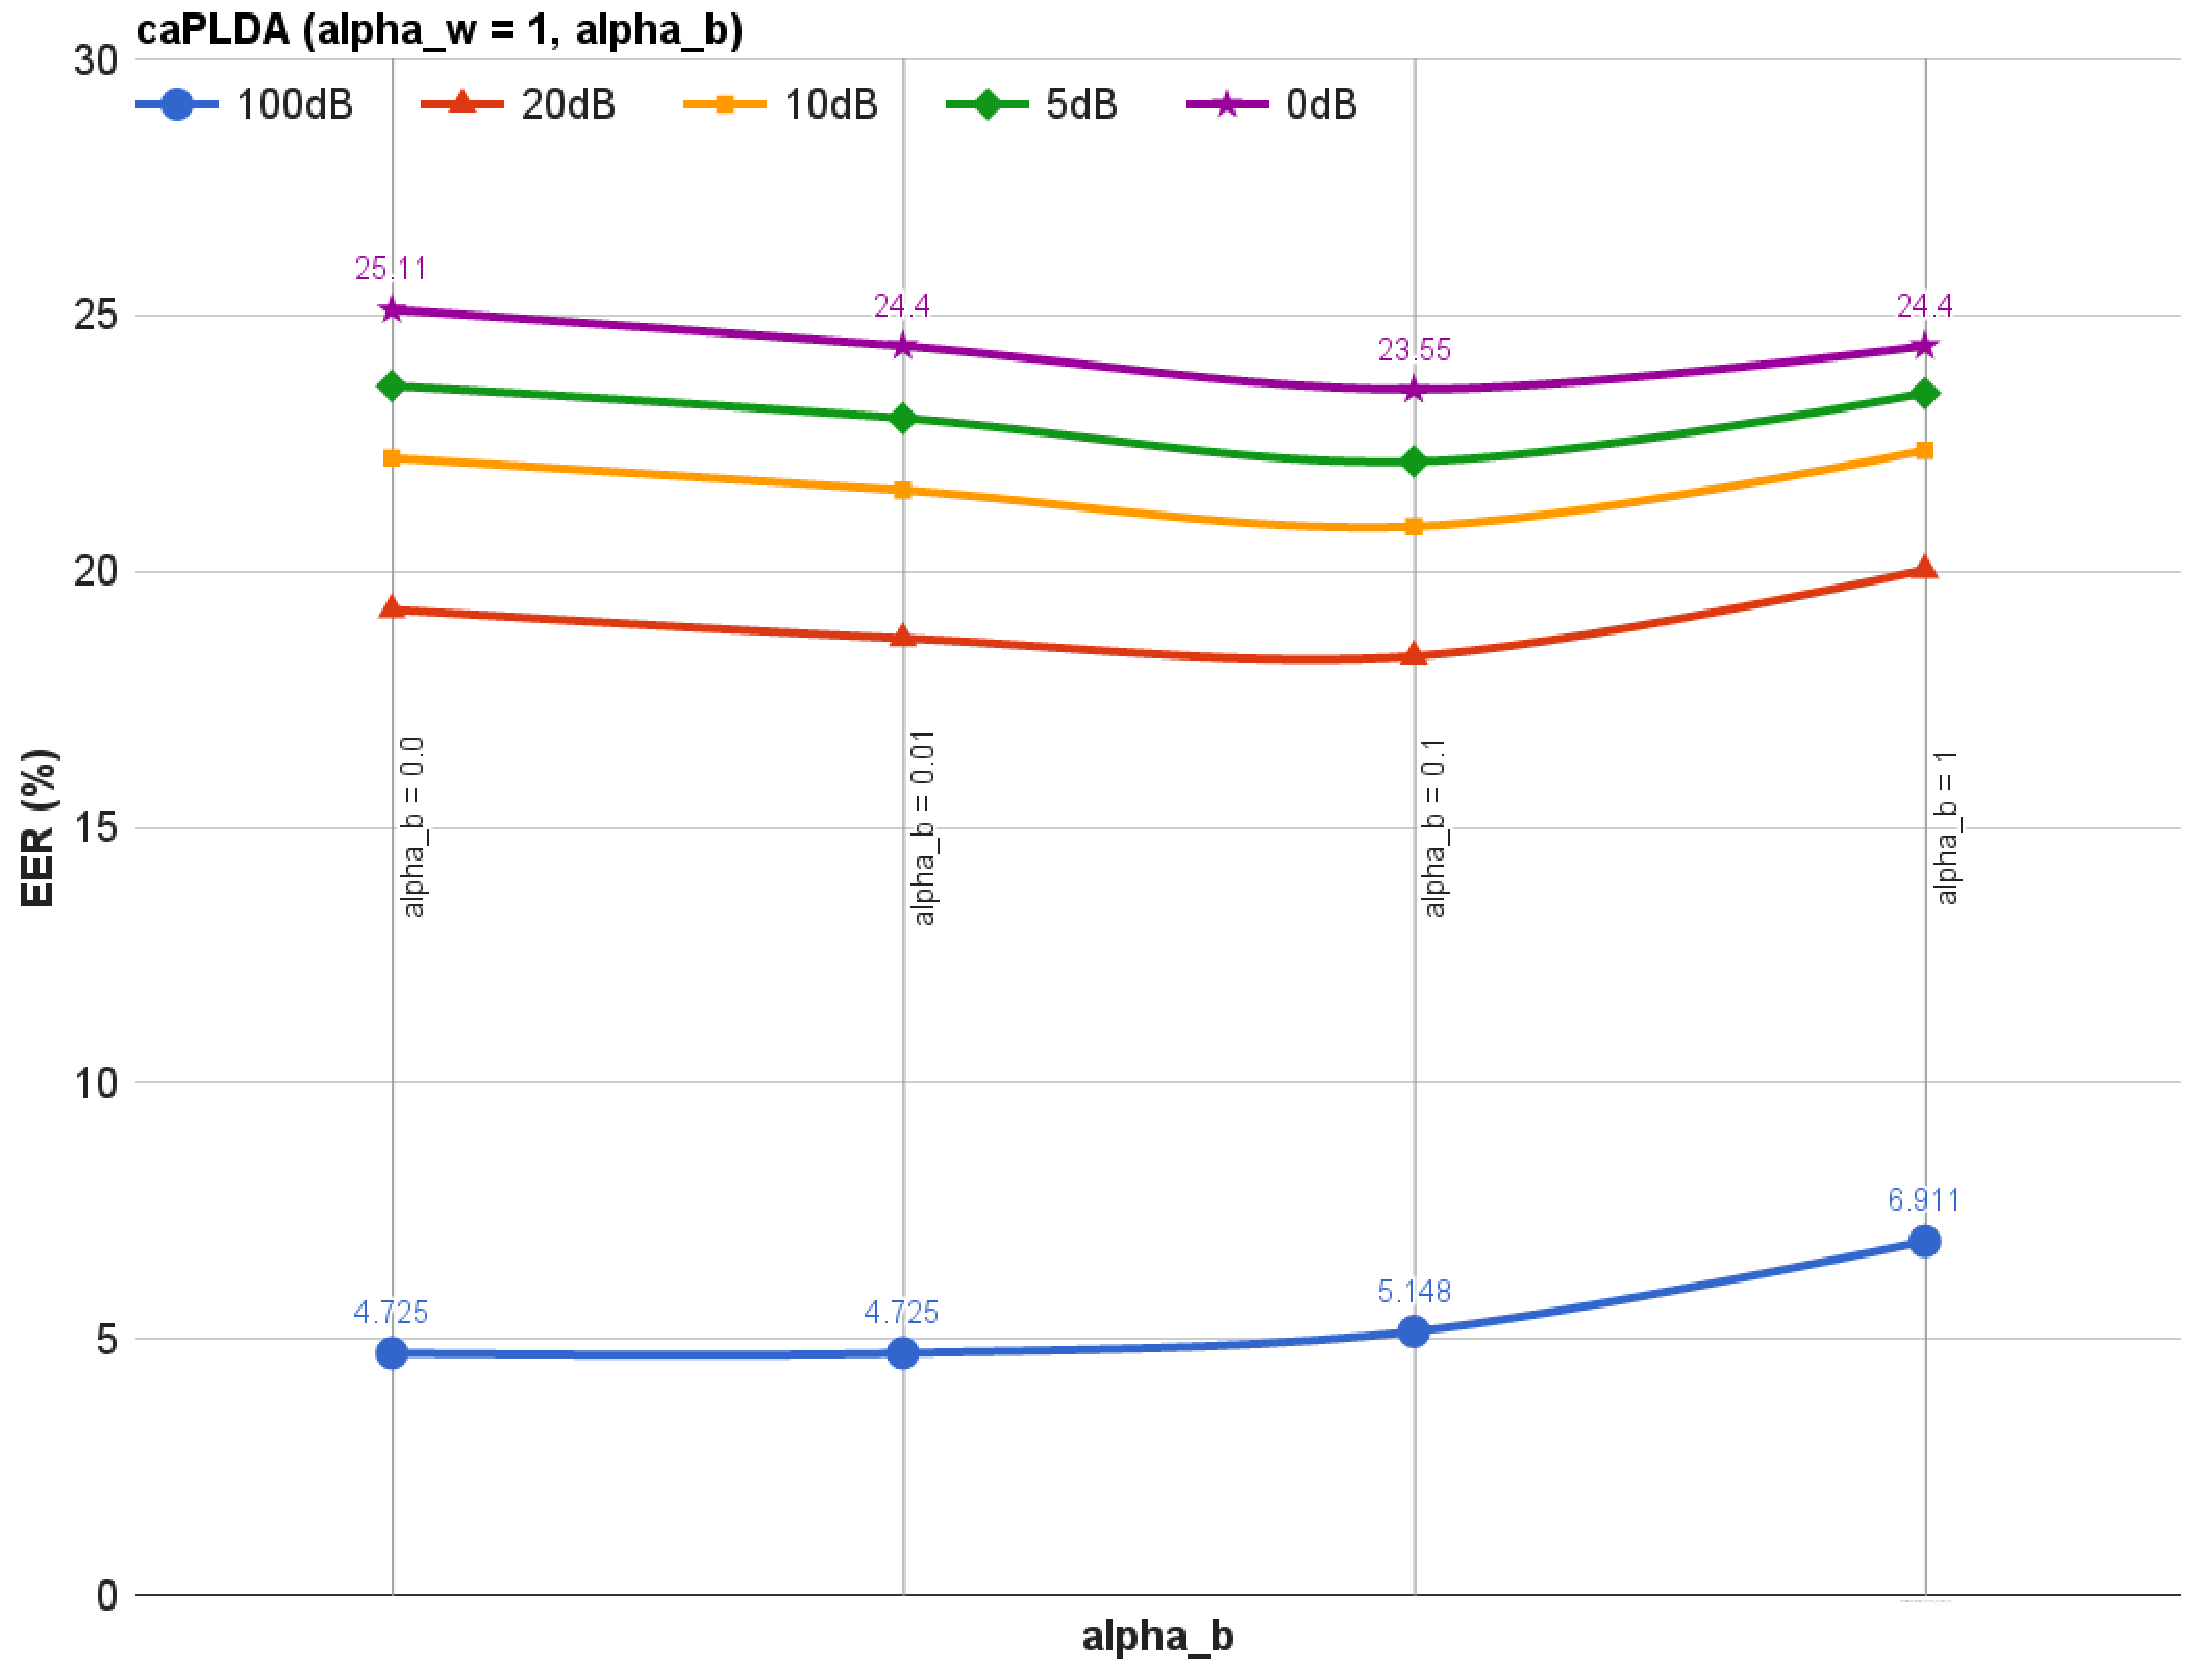
\includegraphics[height = 3.2in, width=0.7\textwidth]{figures/eer_vs_alphab}
	\vspace{-2mm}
	\caption{\it \small Comparing caPLDA for different values of between-speaker coefficient ($\alpha_b$). Here we set $\alpha_w$ to 1. The curves start from left with $\alpha_b = 0$, the scenario equivalent to what is shown in Fig.~\ref{fig:cch_in_sid}. The bottom (blue) lines shows the effect on clean trials, in which modifying simplified PLDA always degrades performance. For co-channel trials, however, setting $\alpha_b$ to non-zero values improves performance for all SIR values.}
	\label{fig:alpha_w_is_1}
	\vspace{-1mm}
\end{figure*}

Our second attempt is to investigate the special case in which $\alpha_w$ is set to $0$ and $\alpha_b=1$, as proposed in Sect.~\ref{ssec:alpha_w_0}. 
We argued that in this scenario the estimate for $\Phi_b$ is likely to be most accurate. 
Table~\ref{tbl:alpha_w_0} compares setting using the three mixed PLDA scenarios plus clean PLDA. 
From the last two columns, mixed PLDA ($0, 100dB$) and clean PLDA, we see that performances are fairly close despite the additional training data in mixed PLDA ($0,100dB$). 

\begin{table*}[h!]
	\small
	\centering
	\resizebox{\textwidth}{!}
	{
	\begin{tabular}{|l|c|c|c|c|c|c|c|c|c|c|c|}
		\hline
		\multirow{2}{*}{SIR (dB)} & \multicolumn{3}{c|}{caPLDA + mixedPLDA(0dB)}          & \multicolumn{3}{c|}{caPLDA + mixedPLDA(0,5,10,20,100dB)}  & \multicolumn{3}{c|}{caPLDA + mixedPLDA(0,100dB)}             & \multicolumn{2}{c|}{caPLDA} \\ \cline{2-12} 
		& \multicolumn{2}{r|}{EER (\%)} & minDCF         & \multicolumn{2}{c|}{EER (\%)} & minDCF             & \multicolumn{2}{c|}{EER (\%)}       & minDCF          & EER(\%)               & minDCF       \\ \hline
		100                       & \multicolumn{2}{c|}{9.03}     & 0.648          & \multicolumn{2}{c|}{7.12}     & 0.554              & \multicolumn{2}{c|}{\textbf{6.63}}  & 0.526           & \textbf{5.71}         & 0.465        \\ \hline
		20                        & \multicolumn{2}{c|}{21.16}    & 0.925          & \multicolumn{2}{c|}{18.55}    & 0.890              & \multicolumn{2}{c|}{\textbf{18.48}} & 0.884           & \textbf{18.83}        & 0.915        \\ \hline
		10                        & \multicolumn{2}{c|}{23.34}    & 0.956          & \multicolumn{2}{c|}{20.94}    & 0.940              & \multicolumn{2}{c|}{\textbf{20.52}} & 0.929           & \textbf{21.65}        & 0.953        \\ \hline
		5                         & \multicolumn{2}{c|}{24.96}    & 0.971          & \multicolumn{2}{c|}{22.21}    & 0.957              & \multicolumn{2}{c|}{\textbf{22.00}} & 0.951           & \textbf{22.57}        & 0.975        \\ \hline
		0                         & \multicolumn{2}{c|}{26.09}    & 0.983          & \multicolumn{2}{c|}{23.62}    & 0.978              & \multicolumn{2}{c|}{\textbf{23.06}} & 0.970           & \textbf{23.70}        & 0.986        \\ \hline
	\end{tabular}
	}
	\caption{caPLDA ($\alpha_w=0$,$\alpha_b=1$) using different co-channel training conditions. The last column show performance without co-channel data in PLDA training.}
	\label{tbl:alpha_w_0}
\end{table*}






\chapter{Speaker Diarization in Co-channel Speech}
\label{chap:spkr_diar}

Throughout the course of this study, part of the agenda has been to acknowledge non-overlapping speech as an important component of co-channel. 
It was shown that distinguishing overlap from co-channel introduces more realistic scenarios to the scope of co-channel speech problems. 
An important example of such problems is conversational speech, a common and realistic form of speech. 
Among the various aspects of analyzing conversations, {\it speaker diarization} is closest to speaker recognition.\footnote{As a reminder for the readers, speaker recognition is the main theme of this thesis.} 
Speaker diarization refers to the task of automatically determining ``who spoke when?'' within an audio signal containing two or more speakers. 
This chapter addresses the tasks of 1) segmenting co-channel data into single-speaker excerpts and 2) clustering segments, which means to group them by speakers. 
Tasks are described within the context of CRSS-SpkrDiar, a speaker diarization tool-kit designed to perform diarization while simultaneously supporting speaker recognition and speech recognition using Kaldi\cite{kaldi}. 
Therefore, the contribution of this chapter is to: 
\begin{itemize}
	\item introduce an end-to-end conversation analysis research platform that is tightly connected to Kaldi and does not require cross-platform coding interfaces. 
\end{itemize}

CRSS-SpkrDiar is a speaker diarization tool-kit developed as part of a collaboration between myself and Chengzhu Yu, a fellow PhD student at the Center for Robust Speech Systems (CRSS). 
The main motivation behind developing this tool-kit is to establish an integrated end-to-end conversation analysis system that provides the capability of diarizing  signals while supporting speech recognition. 
Currently, one of the most popular speech recognition platforms used in research is Kaldi, developed in Johns Hopkins University~\cite{kaldi}. 
Existing diarization systems are implemented in different platforms and to the best of our knowledge none support Kaldi I/O functions. 
Switching between platforms and APIs (Application Programming Interface)  frustrates users who are interested in simultaneously analyzing speaker diarization and speech recognition. 
We hope that developing a speaker diarization module on top of Kaldi will help students and staff with the kind of multi-purpose research that is common in CRSS. 
Although CRSS-SpkrDiar is currently in working condition, as a research platform it is always considered under development and is available for those who are interested in investigating various aspects of conversational data. 

In Sect.~\ref{sec:crssdiar_layout}, a layout of the system and its relationship with Kaldi is presented. 
Section~\ref{sec:crssdiar_layout} also provides a list of our modules and their Input/Output. 
I also explain how these modules interact with Kaldi data types. 
In Sect.~\ref{sec:segmentation}, segmentation, the first task of speaker diarization, is described. 
The purpose of segmentation is to split signals into smaller chunks that contain only one speaker. 
Some segments may contain overlapped speech or no speech at all. 
Therefore, as part of segmentation, speech activity detection (SAD) and overlap detection modules are also integrated into the system. 
In Sect.~\ref{sec:clustering}, the clustering (grouping) module is presented. 
A state-of-the-art technique, called integer linear programming (ILP), is used in CRSS-SpkrDiar to cluster segments obtained from the segmentation stage~\cite{bredin2013ILP}. 
Clustered groups represent segments that belong to the same speaker. Another component also described in Sect.~\ref{sec:clustering} is the re-segmentation, which acts as a correction layer on top of the clustering module. 
Sections~\ref{sec:plda_ilp}~and~\ref{sec:other_distances_ilp} describe some of the novel techniques used to improve clustering performance in CRSS-SpkrDiar. 
Section~\ref{sec:chDrz_evaluation} summarizes some evaluations on the AMI meeting corpus. 
Finally, Sect.~\ref{sec:chDiar_future} points out some of the future work required to further improve CRSS-SpkrDiar. 

Part of the reason this chapter is placed at the end of the dissertation is that it can be viewed as a description of a comprehensive system that contains all of the problems that have been looked at so far. 
Furthermore, since CRSS-SpkrDiar is a research platform that could potentially benefit those looking beyond the scope of this study, I consider it a gateway to future work for my thesis. 



 
\section{CRSS-SpkrDiar Layout}
\label{sec:crssdiar_layout}

The approach in speaker diarization is to split an audio recording (usually at least a few minutes long) into smaller segments that only contain one speaker.
After completing the first step, one must label the segments according to speaker identities. 
The assumption is that no prior knowledge of the number of speakers or their identities is available. 
The only possible solution, therefore, is to compare the segments and group those that appear to belong to the same speaker. 

The segment-and-cluster approach is the most common solution to speaker diarization~\cite{meignier2010lium,anguera2012diarization}. 
That being said, alternative approaches have been proposed. 
Especially with regard to segmentation and post-clustering steps. 
Some studies completely ignore the segmentation step and use equal-length segments to perform clustering~\cite{sell_garcia_2015diarization}. 
Skipping segmentation is an attractive proposition, since as will be shown in the following section, segmentation is prone to errors. 
In addition, using equal lengths instead of varying-length segments to some extent guarantees equal reliability of individual segments for the clustering step. 
We say equally reliable because speaker-dependent features (e.g. i-Vectors) are known to depend largely on the length of the signals from which they are extracted~\cite{hasan2013duration}. 
When automatic segmentation is used to split the audio recording, segment lengths may vary causing the corresponding speaker-dependent features to vary in quality and reliability. 

Another component of speaker diarization, not mentioned above, is the re-segmentation step. 
Re-segmentation is a post-clustering step used to prevent sudden changes in the speaker. 
The reason this module is important is the fact that clustering does not take time sequences into account when grouping segments. 
Meanwhile, as listeners we expect a certain amount of coherence in conversations. 
This presumed coherence in the sequence of speakers is used to correct errors in the clustering step. 

\begin{figure}[t!]
	\centering
	\textbf{Speaker diarization system description}\par\medskip
	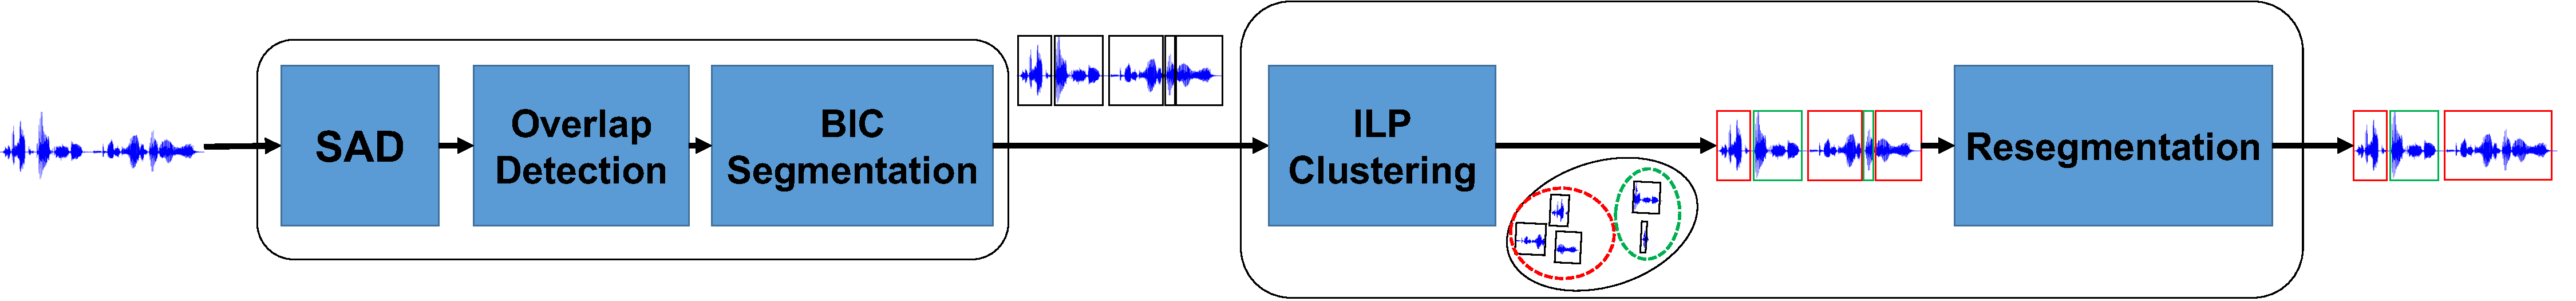
\includegraphics[height = 1in, width=1\textwidth]{figures/crssdiar_outline}
	\caption{ \small CRSS-SpkrDiar system overview. Two main steps are used in speaker diarization: 1) Segmentation (SAD, overlap detection, and BIC segmentation) and 2) clustering (ILP clustering and resegmentation). }
	\label{fig:ch5_crssdiar}
	\vspace{-3mm}
\end{figure}


Figure~\ref{fig:ch5_crssdiar} shows an overview of CRSS-SpkrDiar. 
The input is the audio recording of two or more speakers. 
We start by performing speech activity detection (SAD) and overlap detection to label non-speech and overlapped segments as off-bounds. 
The next step is segmentation, which uses a measure called Bayesian Information Criterion (BIC) to detect speaker change points~\cite{chen1998BIC}. 
After BIC-Segmentation, we have access to segments within the audio recordings and would like to label these segments to determine which belongs to which speaker (speaker A, B, C, etc.). 
Of course, these speaker identities are assigned relative to the input audio and are not actual speaker identities. 
This means that given another input signal, the speaker diarization system will provide similar labels, but speaker A in audio 1 has no relation to speaker A in audio 2. 
CRSS-SpkrDiar generates speaker labels using integer linear programming (ILP) to cluster the segments. 
ILP, described in detail in Sect.~\ref{sec:clustering}, uses a global optimization approach to minimize speaker diversity within each cluster while simultaneously minimizing the number of clusters (aka speakers). 

Thus is the overview of a standard speaker diarization system. 
As mentioned before, there are many implementations available for speaker diarization. 
What CRSS-SpkrDiar offers in addition is to allow speaker diarization in a platform that also supports speech and speaker recognition (Kaldi). 


\subsection{Interaction with Kaldi}
\label{ssec:crssdiar_and_kaldi}

As pointed at the beginning of the chapter, a driving force in developing this tool-kit was high compatibility with the Kaldi speech and speaker recognition platform~\cite{kaldi}. 
For those not familiar with the Kaldi project, it is a toolkit for speech recognition written in C++ and licensed under the Apache License v2.0. Kaldi is intended for use by speech recognition researchers~\cite{kaldi}. 
Kaldi comprises many modules each designated to a specific task. For example, {\it feat} for feature extraction or {\it ivector} for ivector-based speaker recognition. 
Most modules come with a corresponding {\it bin} directory  that contains executable files used to perform various functions in a speech or speaker recognition system (e.g. {\it featbin}, {\it ivectorbin}). 
The executables are those most users interact with in their Bash scripts, which are also referred to as ``recipes''. 

CRSS-SpkrDiar follows the same convention and consists of a {\it diar} and a {\it diarbin} directory. 
The classes are defined in {\it diar}, while {\it diarbin} contains the executables used to perform segmentation and clustering. 
CRSS-SpkrDiar uses matrix and utility libraries from Kaldi in its core.  
Kaldi also includes modules that define Gaussian mixture models and Hidden Markov models ({\it gmm} and {\it hmm}), of which we also take advantage for acoustic modeling. 
As mentioned in the previous section, i-Vectors are used in CRSS-SpkrDiar as speaker-dependent features. 
Therefore, Kaldi's {\it ivector} is used to extract i-Vectors and calculate distances and models such as PLDA (probabilistic linear discriminant analysis) to perform clustering. 
Figure~\ref{fig:ch5_crssdiar_vs_kaldi} shows the interaction between {\it diar} and {\it diarbin} components and Kaldi libraries. 

\begin{figure}[t!]
	\centering
	\textbf{CRSS-SpkrDiar modules}\par\medskip
	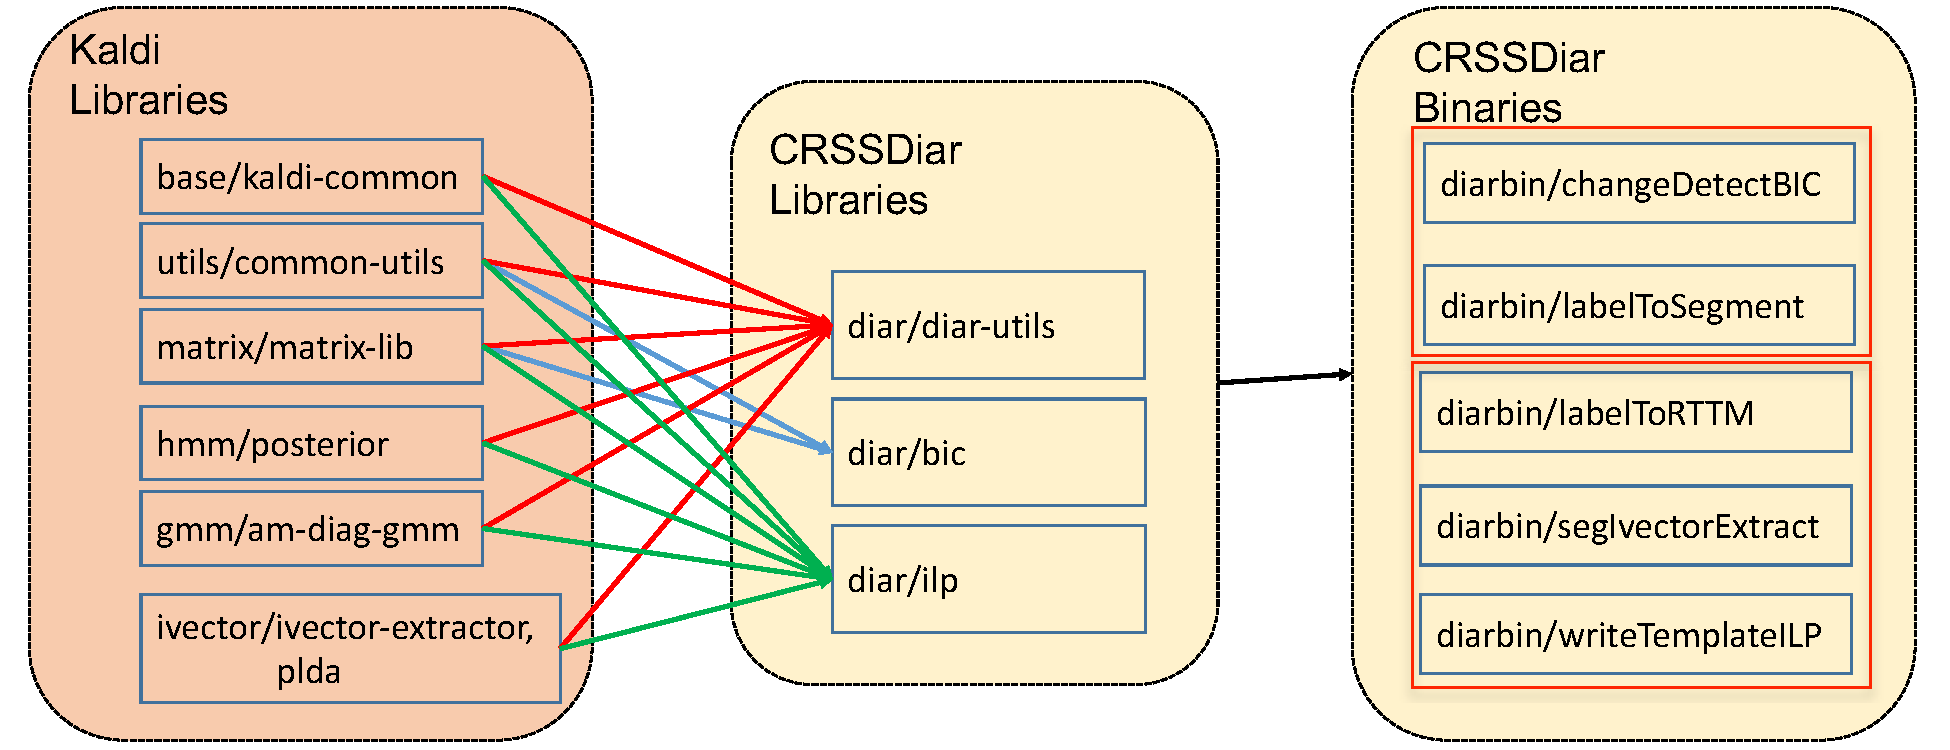
\includegraphics[height = 2in, width=0.8\textwidth]{figures/crssdiar_and_kaldi}
	\caption{ \small CRSS-SpkrDiar components and their relation with Kaldi libraries.  }
	\label{fig:ch5_crssdiar_vs_kaldi}
	\vspace{-3mm}
\end{figure}

\section{Segmentation}
\label{sec:segmentation}
This section briefly describes the layout of the Segmentation component in CRSS-SpkrDiar. 
Traditionally, the approach for speaker diarization has been to first identify speaker change points in an audio stream. 
This is due to the restrictive framework of typical speaker diarization problems. 
The restriction being no prior knowledge of the number or identity of the speakers in the signal. 
Therefore, the solution is to track acoustic features along the signal and detect points at which these features demonstrate significant changes. 

Segmentation in the context of this study is formally defined as detecting the time indexes corresponding to changes in an ordered sequence of acoustic features~\cite{cettolo2005evaluation}. 
One of the most popular speaker change detection algorithms used in speaker diarization is the Bayesian information criterion (BIC), which is briefly described in this section. 
I should point out that BIC segmentation has been thoroughly studied in the research community and several resources are available that substantially cover the essentials required to understand its function in a speaker diarization system~\cite{cettolo2003efficient,cettolo2005evaluation,chen1998BIC}. 
The content here is intended to describe all aspects of CRSS-SpkrDiar and share implementation details for the curious reader. 

\subsection{Bayesian Information Criterion}
\label{ssec:chDiar_secBIC}
The Bayesian information criterion (BIC) is a measure that determines the effectiveness of a given probabilistic model in capturing statistical characteristics of a set of data samples. 
BIC is used in segmentation as a way to quantify the certainty of the existence of a break-point in a given window of the audio. 
Therefore, instead of finding a global solution to the segmentation problem defined in Sect.~\ref{sec:segmentation}, the standard BIC implementation tracks a sliding window in the audio and compares the following two hypotheses: 
\begin{itemize}
	\item $H_0$: The window does not contain a breaking point. 
	\item $H_1$: The window contains exactly one breaking point. 
\end{itemize}

In speaker diarization terms, $H_0$ implies that the window contains one speaker, while $H_1$ implies that two speakers exist. 
BIC segmentation tests these hypotheses by using the following function in a sequence of acoustic features in a window, $\{X_1X_2...X_N\}$, for the hypothesis $H$:
\begin{equation}
BIC(H) = log\mathcal{L}_{M}(H) - P_{M_{N}}, 
\end{equation}
where $\mathcal{L}_{M}(H)$ is the maximum likelihood of the model $M$ under hypothesis $H$. $P_M$ is the BIC penalty function~\cite{schwarz1978BIC} when $M$ is used to parameterize $N$ samples. The indexes correspond to time frames.\footnote{As we know, acoustic features, $X_i$, are calculated over typically $25 msec$ frames. 
The framing used throughout this chapter uses $25 msec$ frames with an increment of $10 msec$. These frames are not to be mistaken with windows used to search for change points.} 
\begin{equation}
P_{M_N} = \frac{F_M}{2}log(N),
\end{equation}
with $F_M$ as the degrees of freedom of the chosen model, $M$. 
When the sequence $\{X_1X_2...X_N\}$ comprises two segments (i.e., $H = H_1$), the break-point is assumed to be an index $i_{max}$ between $1$ and $N$. 
$BIC(H_1)$ is maximized at the break-point $i = i_{max}$. 
This assumption states that breaking the sequence into two sub-sequences $\{X_1X_2...X_{i_{max}}\}$ and $\{X_{i_{max}+1}X_{i_{max}+2}...X_N\}$ maximizes the BIC penalty. 
On the other hand, if the sequence does not contain a break-point (i.e., $H_0$), $i_{max}$ can be assumed equal to $N$. 
The actual measure used in BIC segmentation is the difference between the BIC corresponding to $H_0$ and the BIC of $H_1$. This value is called $\Delta BIC_i$: 
\begin{equation}
\Delta BIC_i = (log \mathcal{L}_{M_i} - P_{M_i}) - (log \mathcal{L}_{M_N} - P_{M_N})
\end{equation}
where $\mathcal{L}_{M_i}$ is short-hand for the maximum likelihood of $H_1$ when the break-point is at index $i$. 
If $\Delta BIC_i > 0$, the model favors $H_1$ at breaking point $i$, and otherwise the model suggests no break-points ($H_0$).  

$\Delta BIC$ Depends on the model chosen for $M$. 
A common choice in speaker diarization is a Gaussian model, which assesses whether the sequence is best described with one covariance matrix ($H_0$) or two ($H_1$). 
In~\cite{cettolo2005evaluation}, $\Delta BIC_i$ is derived for Gaussian modeling with the inclusion of a sensitivity factor $\lambda$. 
\begin{equation}
\label{eq:dbic_gaussian}
\Delta BIC_i = \frac{N}{2} log |\Sigma| - \frac{i}{2} log |\Sigma_1| - \frac{N-i}{2}log |\Sigma_2]| - \lambda P_{M_N}
\end{equation}
where $\Sigma$ is the maximum likelihood estimate of the covariance matrix of $\{X_1X_2...X_N\}$. Similarly, $\Sigma_1$ corresponds to the sequence $\{X_1X_2...X_i\}$ and $\Sigma_2$ to $\{X_{i+1}X_{i+2}...X_N\}$. 
$P_M$ in Eq.~(\ref{eq:dbic_gaussian}) is the BIC penalty of modeling $N$ samples with a Gaussian. 
The number of free parameters in a multi-variate Gaussian is $d + \frac{d(d+1)}{2}$, in which $d$ is the dimension of the acoustic features. 
The degrees of freedom include $d$ values for the Gaussian mean and $\frac{d(d+1)}{2}$ values for the symmetric covariance matrix. 

In addition to identifying whether a window contains one or two speakers, the segmentation module is also expected to return a time index for the change point. 
BIC segmentation returns this value by incrementally increasing the index $i$ until the point at which $\Delta BIC_i$ is positive. 
Once the change point is detected, granted that it exists in the first place, a recursive search is conducted with smaller increments to find the exact change point. 

Now that the background theory of BIC segmentation has been presented, we move on to a description of BIC segmentation in CRSS-SpkrDiar in a module called change-point detection. 

\subsection{Change-Point Detection in CRSS-SpkrDiar}
Change-point detection, or change detection in short, is a tool used to estimate segment boundaries in an audio stream. 
It performs BIC segmentation on speech segments produced from speech activity and overlap detection. 
From here on speech segments refer to segments that may contain multiple non-overlapping speakers or a single speaker. 
The no-overlapping property is implied unless ``overlapped segments'' is used. 
The goal is to split segments at locations where speakers change. 
There is no prior assumption regarding the number of speakers in any given segment. 
The output of change detection, however, will ideally produce smaller segments that each contain only one speaker. 

Given a segment, change detection first examines whether the segment is long enough to compute reliable BIC estimates (as defined in Sect.\ref{ssec:chDiar_secBIC}). 
For segments that are sufficiently long, a sliding window is defined that incrementally grows in size. 
This window will grow until: 1) either a change point is detected using the $\Delta BIC$ measure from Eq.~(\ref{eq:dbic_gaussian}) or 2) the length of the window reaches a maximum acceptable length at which point the window is assumed to contain only one speaker (no change points are detected). 
As mentioned, the window slides until it reaches the end of the segment and returns the change points that were found during the search. 

Every time a change point is detect the window first performs an identical search with more refined search increments until it finds the feature index, $i$, at which $\Delta BIC_i$ is maximized. 
After finding $i_{max}$, the window is reset and continues the search at $i_{max}+1$. 

Figure~\ref{alg:changedetection} shows the pseudo-code for change detection implemented in CRSS-SpkrDiar. 
The algorithm requires a set of user defined parameters that determine the search speed and BIC sensitivity. 
\begin{itemize}
	\item $N_{min}$: minimum window length (in number of frames) used to start search for change point. Segments shorter than this value are not long enough to estimate $\Delta BIC$. 
	\item $N_{max}$: maximum window length. The search window grows incrementally until it reaches this maximum length. If the search window reaches this value before a change point is detected, the algorithm quits the search and declares no change point. 
	\item $N_{margin}$: window margin. These margins are used to assure that sufficient number of frames are available to compute BIC estimates. 
	\item $N_{second}$: refining window length. Once a change-point is detected, the search is refined using a smaller window of this length. 
	\item $N_{shift}$: sliding parameter. The window slides to the right once its length reaches $N_{max}$. 
	\item $N_{grow}$: The incremental growth factor. Every time a window is examined for change points, the window length increases by $N_{grow}$.
	\item $\lambda$: BIC sensitivity factor. The higher this value, the more sensitive $\Delta BIC$ is to changes. 
	\item $lowResolution$: initial search increment used to calculate $\Delta BIC_i$. The value $i$ increments by $lowResolution$ in each iteration.
	\item $highResolution$: refined search increment. After a change point is detected in the initial search, a second search window is created and search with an increment of $highResolution$. 
\end{itemize}

\begin{figure}
\begin{lstlisting}
SplitSegment
// Perform BIC change dectect on single speech segment.
if (Nmin >= segment.Length) 
	return
window.Create(segment.Start + Nmargin,Nmin)

while (window.End <= segment.End) 
	maxBICIndexValue = DeltaBIC(window, lowResolution)
	while (maxBICIndexValue <= 0 & window.Length < Nmax) & window.End <= segment.End) 
		window.GrowWindow(Ngrow)
		maxBICIndexValue = DeltaBIC(window,lowResolution)
		
	while (maxBICIndexValue <= 0 & window.End <= segment.End) 
		window.ShiftWindow(Nshift)
		maxBICIndexValue = DeltaBIC(window,lowResolution);
	
if (maxBICIndexValue.second > 0  & window.End <= segment.End) 
	window.Restart(Nsecond)
	maxBICIndexValueHighRes = DeltaBIC(window, highResolution)
	if (maxBICIndexValueHighRes.second > 0) 
		i_max = maxBICIndexValueHighRes.Index
		bicSegments.Create([segment.Begin,i_max]);
		segment.Begin = i_max + 1;
		window.ResetWindow(segment.Begin,Nmin);
else 
	window.ResetWindow(segment.End - Nmargin + 1, Nmin)
\end{lstlisting}
\caption{Algorithm - change detection using BIC. The algorithm describes the two-step procedure of searching for change points in an audio segment. The first step is to search for change points using larger increments, $lowResolution$. Once the change point is detected, a second, more refined, search is performed in a smaller search window using $highResolution$.}
\label{alg:changedetection}
\end{figure}

An important component of change detection is the {\it segment} data type. 
This class contains all the necessary information to calculate functions used in speaker diarization. 
For example, each {\it segment} contains two variables, {\it Begin} and {\it End} that indicate the start and end frames corresponding to that segment. 
This class also includes functions used to calculate i-Vectors, which will be used extensively in the next section. 
{\it Segments} is considered the core data type used in CRSS-SpkrDiar and is highly compatible with existing Kaldi classes. 

\newpage
\section{Clustering}
\label{sec:clustering}
This section describes the second step in speaker diarization, clustering the segments. 
After single-speaker segments are identified, the speaker diarization system must decide which segments belong to the same speaker. 
This is accomplished without prior knowledge of the number of speakers or their identities. 
The task of grouping segments that belong to the same speaker is known as clustering. 

A number of bottom-up and top-down solutions have been suggested for the clustering step in speaker diarization~\cite{tranterreynolds2006drzoverview,anguera2012DRZreview}. 
Top-down approaches start by assuming that all segments belong to a single cluster and iteratively split clusters into smaller, more exclusive, groups. 
Bottom-up clustering, on the other hand, starts by assuming each sample is a separate cluster and iteratively merges clusters into more inclusive groups. 
The most popular of these is a bottom-up algorithms called hierarchical agglomerative clustering (HAC). 
This approach first assumes that all segments belong to a separate cluster (i.e., speaker) and iteratively merges the two closest clusters. 
A similarity criterion is used to measure the distance between clusters. 
Performance varies depending on the criterion used (e.g., BIC, Kullback-Leibler divergence). 
This iterative process continues until the similarity criterion is no longer satisfied between any two clusters. 
As opposed to the single multivariate Gaussian used to detect change points in the previous section, the clustering process usually uses more sophisticated measures. 
Gaussian mixture models (GMM) have been proven effective in modeling clusters~\cite{zelenak2010albayzin}. 
As clusters merge, the amount of data available to estimate GMM parameters increases. 
Therefore, GMM reliability increases in HAC iterations. 
It is easy to see why using GMMs was not feasible in the segmentation step, since the amount of data was too little to model an entire GMM. 

Despite its popularity, HAC is associated with a number of issues. 
The most important being the error-propagation that occurs during iterations. 
If two segments are incorrectly grouped together in one iteration, the model (e.g., GMM) used to represent the cluster for the next iteration will not accurately represent the speaker identity, and so on. 
This issue has led many to use other top-down clustering approaches, which are less likely to suffer from error-propagation. Examples being K-means~\cite{shum2011exploiting} or spectral clustering~\cite{shum2012spectralclustering, ning2006spectral}. 
To the best of our knowledge, there are no conclusive results that suggest one clustering method over all others for speaker diarization. 
Another important development with regard to clustering has been to use i-Vectors to perform clustering. 
The standard HAC-GMM framework does not use i-Vectors in the clustering process. 
Some developments have been made to use i-Vector distances in an HAC clustering solution. 
The reader should be reminded that the compatibility of CRSS-SpkrDiar with Kaldi allows for a complete integration of i-Vectors with clustering.\footnote{While this manuscript was under preparation, HAC was also added to CRSS-SpkrDiar. The most current version of the software supports both HAC and ILP clustering methods.} 

An increasingly popular algorithm that has been used in speaker diarization has been {\it integer linear programming} (ILP). 
Two reasons that make ILP particularly interesting are: 
\begin{itemize}
	\item Given appropriate formulation, ILP can result in global optimum for some clustering problems. 
	\item A vast bed of research exists for linear programming algorithms. Integrating these solutions into any problem, in this case speaker diarization, provides new insights and advantages. 
\end{itemize}

ILP was introduced as a global optimization solution for the clustering problem in speaker diarization by Rouvier and Meignier~\cite{rouvier2012ilp}. 
An attractive aspect of ILP for speaker diarization is that it is relatively strait-forward to perform ILP clustering on i-Vectors~\cite{dupuy2012ivectorsILP}. 
The implementation in CRSS-SpkrDiar is based on improvements on the original ILP formulation for speaker diarization~\cite{dupuy2014ILPimprovement}. 

The single-speaker segments from change detection can be used to derive i-Vectors. 
As you may recall from Chapter~\ref{chapter:backend}, i-Vectors are fixed-length vectors that represent speaker-specific characteristic of a given audio signal of variable length. 
ILP is a constrained optimization problem that determines which i-Vectors should fall in the same cluster. 
The optimization ensures that:
\begin{enumerate}
	\item all i-Vectors in a cluster are within a predefined distance, $\delta$, of all the other i-Vectors in that cluster. 
	\item the number of clusters is minimal. 
	\item every i-Vector is assigned to one and only one cluster. 
\end{enumerate}

The inherent compatibility of ILP allows formulating the aforementioned conditions in a convex linear programming manner, regardless of the non-linearities of distance metrics. 
The linearity comes from the fact that distance measures are assumed pre-calculated and do not depend on the choice of clusters. 
It was mentioned before that in AHC, the choice of cluster members in each iteration modified the distances, since it affected the cluster model for the next iteration. 
The same applies to top-down clustering, such as K-means. 
However, distances in ILP are constant and do not depend on the cluster labels. 
Therefore, ILP claims to provide a global minimum to the following equation derived form conditions (1) and (2) from the list above: 

for clusters $C \in \{1 ... N\}$:

\begin{equation}
\label{eq:ilp_minimization}
minimize \hspace{0.2in} \frac{1}{\delta}\sum\limits_{i=1}^{N}\sum\limits_{j=1}^{N}dist(i,j)x_{i,j} + \sum\limits_{k=1}^{N}x_{k,k}
\end{equation}
The minimization problem searches for elements of a binary $N\times N$ clustering assignment matrix, in which $N$ corresponds to the number of i-Vectors (i.e., segments) generated in Sect.~\ref{sec:segmentation}. 
The value $x_{i,i}$ is $1$ if the $i^{th}$ i-Vector is identified as a cluster centroid and $0$ otherwise. 
$x_{i,j}$ is $1$ if the $j^{th}$ i-Vector belongs to the cluster whose centroid is $i$. 
The first term in Eq.~(\ref{eq:ilp_minimization}) makes sure that centroids are picked in a way that minimizes the sum of distances of all elements in a cluster from their assigned centroid. 
The distance between the $i$ and $j^{th}$ i-Vectors is $dist(i,j)$. 
Clearly, the optimal solution to only minimize the first term, $\frac{1}{\delta}\sum\limits_{i=1}^{N}\sum\limits_{j=1}^{N}dist(i,j)x_{i,j}$, is to choose all i-Vectors as a centroid, which will undesirably result in $N$ clusters. 
Hence, the second term is introduced to simultaneously minimize the number of clusters. $\sum\limits_{k=1}^{N}x_{k,k}$ is the sum of diagonal elements, also equal to the number of clusters. 
The first term is normalized by a factor $\delta$. 
This normalizing factor is the threshold used as the radius for all clusters. 
To assure that all clustering conditions are satisfied, a set of constraints are added to Eq.~(\ref{eq:ilp_minimization}). 
Some conditions are implied by the formulation, such as: 
\begin{equation}
x_{i,j} \in \{0,1\},  \hspace{1in}  1 \leq i,j \leq N
\end{equation}
which states that the clustering assignment matrix must have binary elements; hence the phrase {\bf integer} linear programming. 
Some constraints are straight-forward, for example each i-Vector can only be assigned to one cluster: 
\begin{equation}
\sum\limits_{i=1}^{N}x_{i,j} = 1, \hspace{1in} 1 \leq i \leq N
\end{equation}
or that all distances should be less that a pre-determined threshold, $\delta$: 
\begin{equation}
d(i,j)x_{i,j} < \delta. \hspace{1in} 1 \leq i,j \leq N
\end{equation}
A more subtle constraint is that an i-Vector $j$ is assigned to a cluster only if the cluster has a centroid. In other words, $j$ can be assigned to $k$ if $k$ is a centroid. 
\begin{equation}
x_{k,j} - x_{k,k} \leq 0. \hspace{1in} 1 \leq k,j \leq N
\end{equation}

The minimization problem can be reformulated into a more compact problem~\cite{dupuy2014ILPimprovement}. 
Using compact solutions with more restrictive constraints reduces the number of variables that need to be solved in the linear programming problem. 
The following formulation increases the speed of the ILP solver by limiting the number of restrictive variables in Eq.~(\ref{eq:ilp_minimization}). For $j \in \{1 ... N\}$ let $K_j = \{k | d(k,j) < \delta\}$ 




\begin{equation}
\label{eq:ilp_minimization_1}
\begin{split}
minimize \hspace{0.2in}& \frac{1}{\delta}\sum\limits_{j=1}^{N}\sum\limits_{k\in K_j}dist(k,j)x_{k,j} + \sum\limits_{k=1}^{N}x_{k,k} \\
subject~to:  \hspace{0.2in}& x_{k,j} \in {0,1}, \hspace{1in} k \in K_j , 1 \leq j \leq N \\
 & \sum\limits_{k\in K_j}x_{k,j} = 1, \hspace{1.2in} 1 \leq j \leq N \\
 & x_{k,j} - x_{k,k} < 0. \hspace{0.5in} k \in K_j , 1 \leq j \leq N`
\end{split}
\end{equation}

The optimzation problem in Eq.~(\ref{eq:ilp_minimization_1}) is implemented in CRSS-SpkrDiar using the GNU linear programming kit (GLPK)~\cite{makhorin2008glpk}. GLPK is an open-source C++ library (As mentioned before, the entire CRSS-SpkrDiar module solely depends on C++ libraries). 
GLPK explicitly reads the objectives, equalities, and inequalities in the form provided in Eq.~(\ref{eq:ilp_minimization_1}). 
To create the input file for GLPK, i-Vectors are extracted from the segments and indexed appropriately. 
A distance matrix (see Sect.\ref{sec:plda_ilp} and \ref{sec:other_distances_ilp}) is calculate using all segment i-Vectors. 
Figure~\ref{fig:ch5_ilp_clustering} summarizes the process of generating the GLPK input, we is called the {\it GLPK Template} in CRSS-SpkrDiar. 

\begin{figure}[ht!]
	\centering
	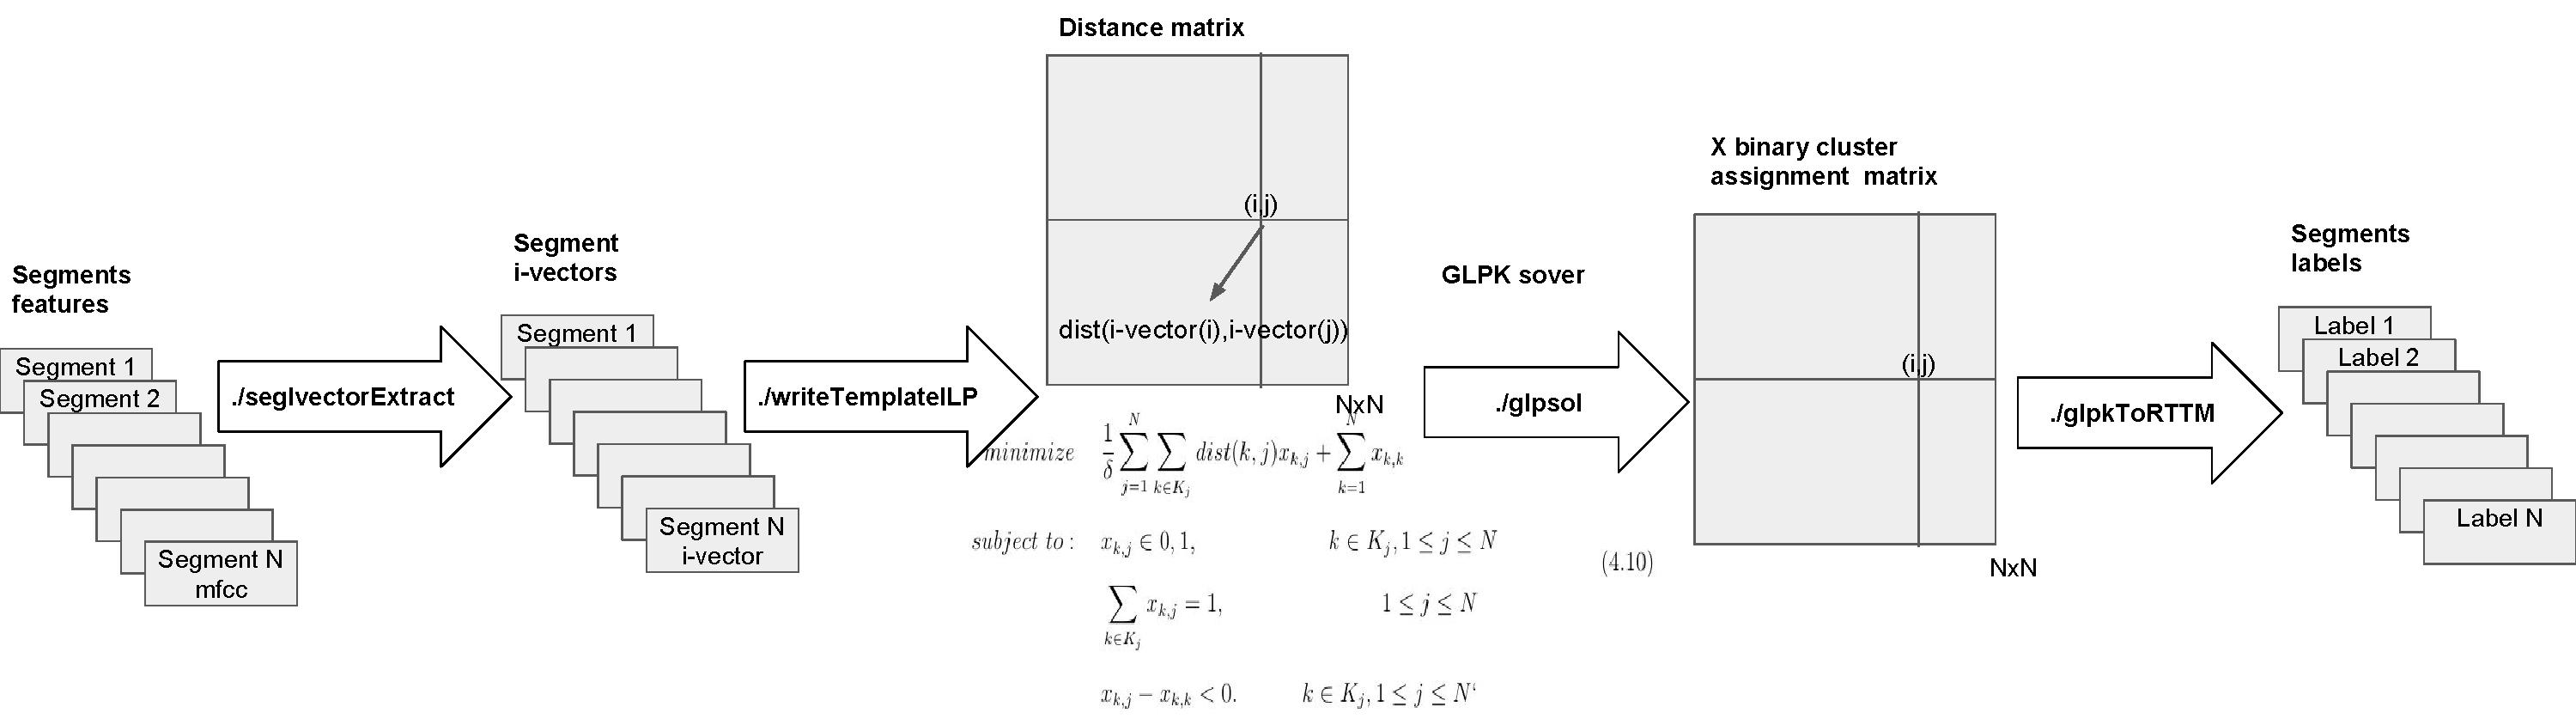
\includegraphics[height = 2.6in, width=1\textwidth]{figures/ilp_clustering_summary}
	\caption{ \small Summary of ILP clustering using CRSS-SpkrDiar. The binary executables used for each step are shown in the figure. }
	\label{fig:ch5_ilp_clustering}
	\vspace{-3mm}
\end{figure}


The descriptions provided in this section were based on existing studies~\cite{mueller2010ILP, rouvier2012ilp,dupuy2012ivectorsILP,dupuy2014ILPimprovement}. 
What was presented here was a brief of summary of existing publications. 
A novel addition in CRSS-SpkrDiar has been in the choice of distance metric, $dist(.,.)$, described in the next section. 

\section{PLDA in ILP clustering}
\label{sec:plda_ilp}
Probabilistic linear discriminant analysis (PLDA) was thoroughly investigated in Chapter~\ref{chapter:backend} as a way to determine whether two individual i-Vectors (or two groups of i-Vectors) belong to the same speaker. 
The same question is faced during the clustering process for speaker diarization. 
Since ILP does not add any restrictions on the distance measures (see Eq.~(\ref{eq:ilp_minimization_1})), PLDA can be used here as the distance metric, $dist(.,.)$. 
This creates a more appropriate setting for the clustering step, which aims to compare speaker identities across segments. 

The use of PLDA in speaker diarization has been proposed in a number of studies~\cite{prazak2011PLDAdrz, silovsky2011PLDAdrz, sell2014PLDAdrz}. 
PLDA proves particularly useful in a class of speaker diarization problems that perform cross-session diarization. 
Cross-session diarization simultaneously clusters segments from several audio streams. 
In this scenario PLDA functions as a channel compensation algorithm. 
CRSS-SpkrDiar proposes to use PLDA as a distance measure to perform global optimization in ILP clustering. 
This is expected to improve performance relative to Mahalanobis and cosine distances previously proposed for ILP clustering~\cite{dupuy2012ivectorsILP,dupuy2014ILPimprovement}. 

CRSS-SpkrDiar accepts labeled background i-Vectors to train a PLDA model (using Kaldi's PLDA class) to calculate distances. 
The function {\it computeDistanceMatrix}  calculates PLDA distances from segment i-Vectors and background i-Vectors in {\it writeTemplateILP}. 
In addition to {\it computeDistanceMatrix} for PLDA, CRSS-SpkrDiar also calculates cosine distance, Mahalanobis distance, and conditional Bayes distance. 
Section~\ref{sec:other_distances_ilp}

\section{Other distance measures}
\label{sec:other_distances_ilp}
In addition to PLDA, three other distance measures are implemented for the clustering procedure in CRSS-SpkrDiar. 

The first is cosine distance, which uses the normalized dot product of i-Vector pairs to define similarity. The cosine distance between two i-Vectors ${\bf v_i}$ and ${\bf v_j}$ is: 
\begin{equation}
\label{eq:cosine_distance}
dist_{cos}(i,j) = \frac{<{\bf v_i} , {\bf v_j} >}{|| {\bf v_i} ||||{\bf v_j}|| }
\end{equation}
Cosine distance in its raw format defined in Eq.~(\ref{eq:cosine_distance}) is slightly incompatible with the distance metric required in Eq.~(\ref{eq:ilp_minimization_1}). 
The problem is that higher cosine distance is associated with closer vectors. Also, $dist_{cos}$ allows negative values. 
ILP minimization, on the other hand, considers lower distance values (starting from $0$) as close vectors and higher values (always positive) as distant. 
Therefore, the cosine metric used in CRSS-SpkrDiar is actually $1 - dist_{cos}(i,j)$. 

The second distance metric is Euclidean distance, defined as the norm-2 distance between ${\bf v_i}$ and ${\bf v_j}$. Similarly, a Mahalanobis distance, which is a weighted Euclidean distance is also applicable. The weight for Mahalanobis distance is calculated from the covariance estimate of all the i-Vectors obtained from segments, ${\bf \Sigma}$. 
\begin{equation}
dist_{mah}(i,j) = \sqrt{({\bf v_i} - {\bf v_j})^T{\bf \Sigma}^{-1}({\bf v_i} - {\bf v_j})}
\end{equation}
For Euclidean distance ${\bf \Sigma} = {\bf I}$. 

The last distance measure is conditional Bayes. This distance was suggested by Rouvier and Meignier~\cite{rouvier2012ilp}} as a substitute for Mahalanobis distance. 
Instead of calculating ${\bf \Sigma}$ from the segment i-Vectors, labeled development i-Vectors are used from an external dataset. 
This measure computes a Mahalanobis distance using the within-class covariance corresponding to development speakers. 
The development data contains groups of i-Vectors from different speakers, for which speaker labels are available. 
The within-class covariance is calculated by averaging the covariance obtained from the i-Vectors of each development speaker. 
The implied assumption here is that all speaker classes have a similar within-class covariance. 
The goal of conditional Bayes is to remove channel-dependent variabilities from the i-Vectors. 

 
\section{Evaluation}
\label{sec:chDrz_evaluation}
This section shows preliminary results from CRSS-SpkrDiar. 
The experiments are conducted on the AMI meeting corpus, briefly described in Chapter~\ref{chapter:backend}. 
AMI consists of audio recordings from meetings, typically $30 min$ sessions. 
The corpus also provides additional background information, including individual speakers' speech recorded from head-set and lapel microphones. 
In addition to audio files, the corpus contains segmentation ground-truth for speaker diarization. 
CRSS-SpkrDiar uses this information to calculate diarization error rates (DER) for each session separately. 
The way CRSS-SpkrDiar addresses different datasets is very similar to Kaldi. 
In that CRSS-SpkrDiar binaries are independent of the data-set, but users can create recipe scripts that are specific to a particular corpus design. 

\subsection{Diarization Error Rates}
\label{ssec:der}
The most popular error rate proposed for speaker diarization is diarization error rate (DER)~\cite{anguera2012DRZreview}. 
This error rate is a combination of three types of errors made by a speaker diarization system. The errors include:  
\begin{itemize}
	\item false alarm errors -- segments that are falsely detected as speech segments,
	\item miss errors -- segments that contain speech from one of the speakers, but are missed (flagged non-speech) by the diarization system, 
	\item speaker error -- clustering error, which incorrectly labels segments, 
\end{itemize}

The last type of error is the most difficult to verify, since the diarization system has no prior knowledge of speakers and therefore assigns its own labels to segments. 
Hence, the labeling produced by the diarization system does not correspond to labels from ground-truth. The figure below shows an example problem. It shows all three types of error in a diarization system (false-alarm, miss, and incorrect labeling of speakers). 
Figure~\ref{fig:ch5_diarization_der} highlights the types of error that are made during diarization. 

\begin{figure}[h!]
	\centering
	\textbf{Speaker Diarization Errors}\par\medskip
	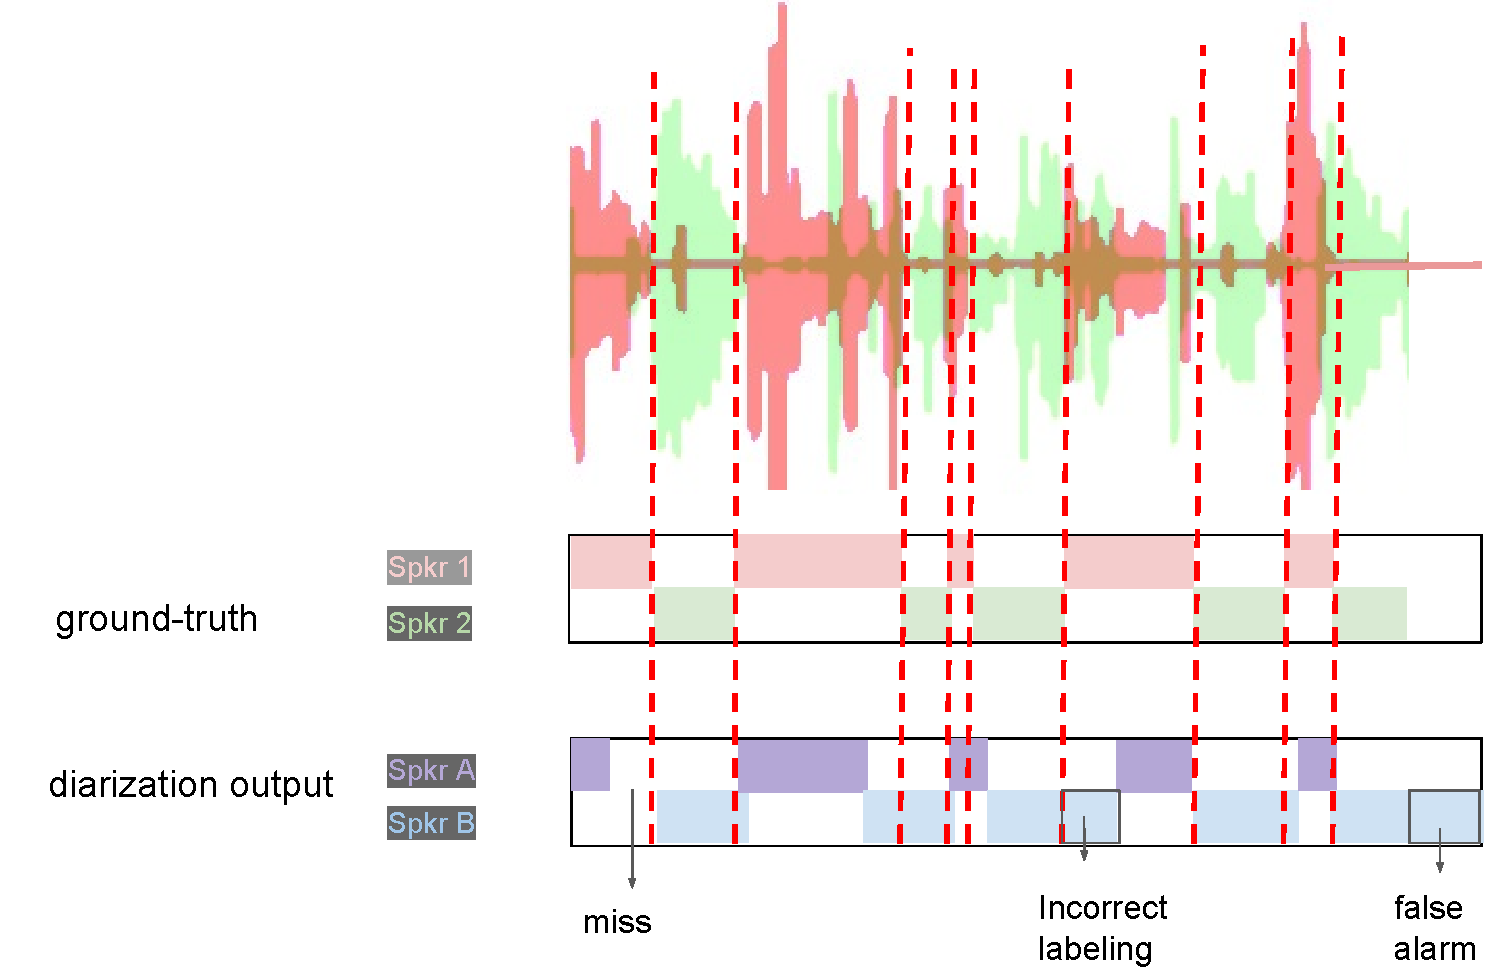
\includegraphics[height = 3.5in, width=1\textwidth]{figures/diarization_example_der}
	\caption{ \small Shows three types of errors made by a diarization system. 1) false alarms: segment that does not contain speech is labeled by diarization system. 2) miss: segment containing speech is not labeled by diarization system. 
		3) incorrect labeling: the third type of error assumes that A is 1 and B is 2. It is up to the diarization error rate calculator to make this assignment.}
	\label{fig:ch5_diarization_der}
	\vspace{-3mm}
\end{figure}

It is also shown that the labels assigned by the speaker diarization system ($A, B$) are different from ground-truth labels ($1, 2$). 
It is up to the diarization error rate calculator to recognize the correct label correspondence, $A:1$ and $B:2$. 
This is done by considering all possibilities, in this case $(A:1,B:2)$ and $(A:2,B:1)$, and returning the assignment that results in minimum labeling error. 


The formulation proposed by NIST for diarization error rate is~\cite{anguera2012DRZreview}:\footnote{Unfortunately, NIST has removed the online evaluation plan from its website. The equations provided here are from Xavier Anguera's PhD thesis~\cite{anguera2007phd}.}
\begin{equation}
DER = E_{spkr} + E_{miss} + E_{fa}, 
\end{equation}
where: 
\begin{equation}
E_{spkr} = \frac{\sum\limits_{s=1}^{S} dur(s)(min(N_{groundtruth}(s),N_{diarization})-N_{correct}(s))}{T_{score}}
\end{equation}
\begin{equation}
E_{fa} = \frac{\sum\limits_{s=1}^S dur(s)(N_{diarization}(s)-N_{groundtruth}(s))}{T_{score}}
\end{equation}
\begin{equation}
E_{miss} = \frac{\sum\limits_{s=1}^S dur(s)(N_{groundtruth}(s) - N_{diarization}(s))}{T_{score}}
\end{equation}
in which $S$ is the total number of segments. The variable $dur(s)$ is the duration of segment $s$. $N_{groundtruth}(s)$ is the number of speakers in segment $s$ provided by the ground-truth. 
$N_{diarization}(s)$ is the number of speakers in segment $s$ hypothesized by the diarization system. 
$N_{correct}(s)$ is the number of speakers correctly matched by the diarization system. 
Finally, $T_{score}$ is the total scoring time. 

CRSS-SpkrDiar uses an evaluation Perl script provided by NIST that calculates DER alongside the individual errors described above. 
This script requires a certain input format for the labels, called rich transcription time marks (RTTM). 
CRSS-SpkrDiar contains labelToRTTM and glpkToRTTM binaries that convert Kaldi vectors to RTTM format. 
The output of the GLPK clustering module can also be converted into RTTM using glpkToRTTM. 

\subsection{Comparing distance measures}

\begin{figure}[b!]
	\vspace{2mm}
	\centering
	\textbf{DER for different distance measures in CRSS-SpkrDiar}\par\medskip
	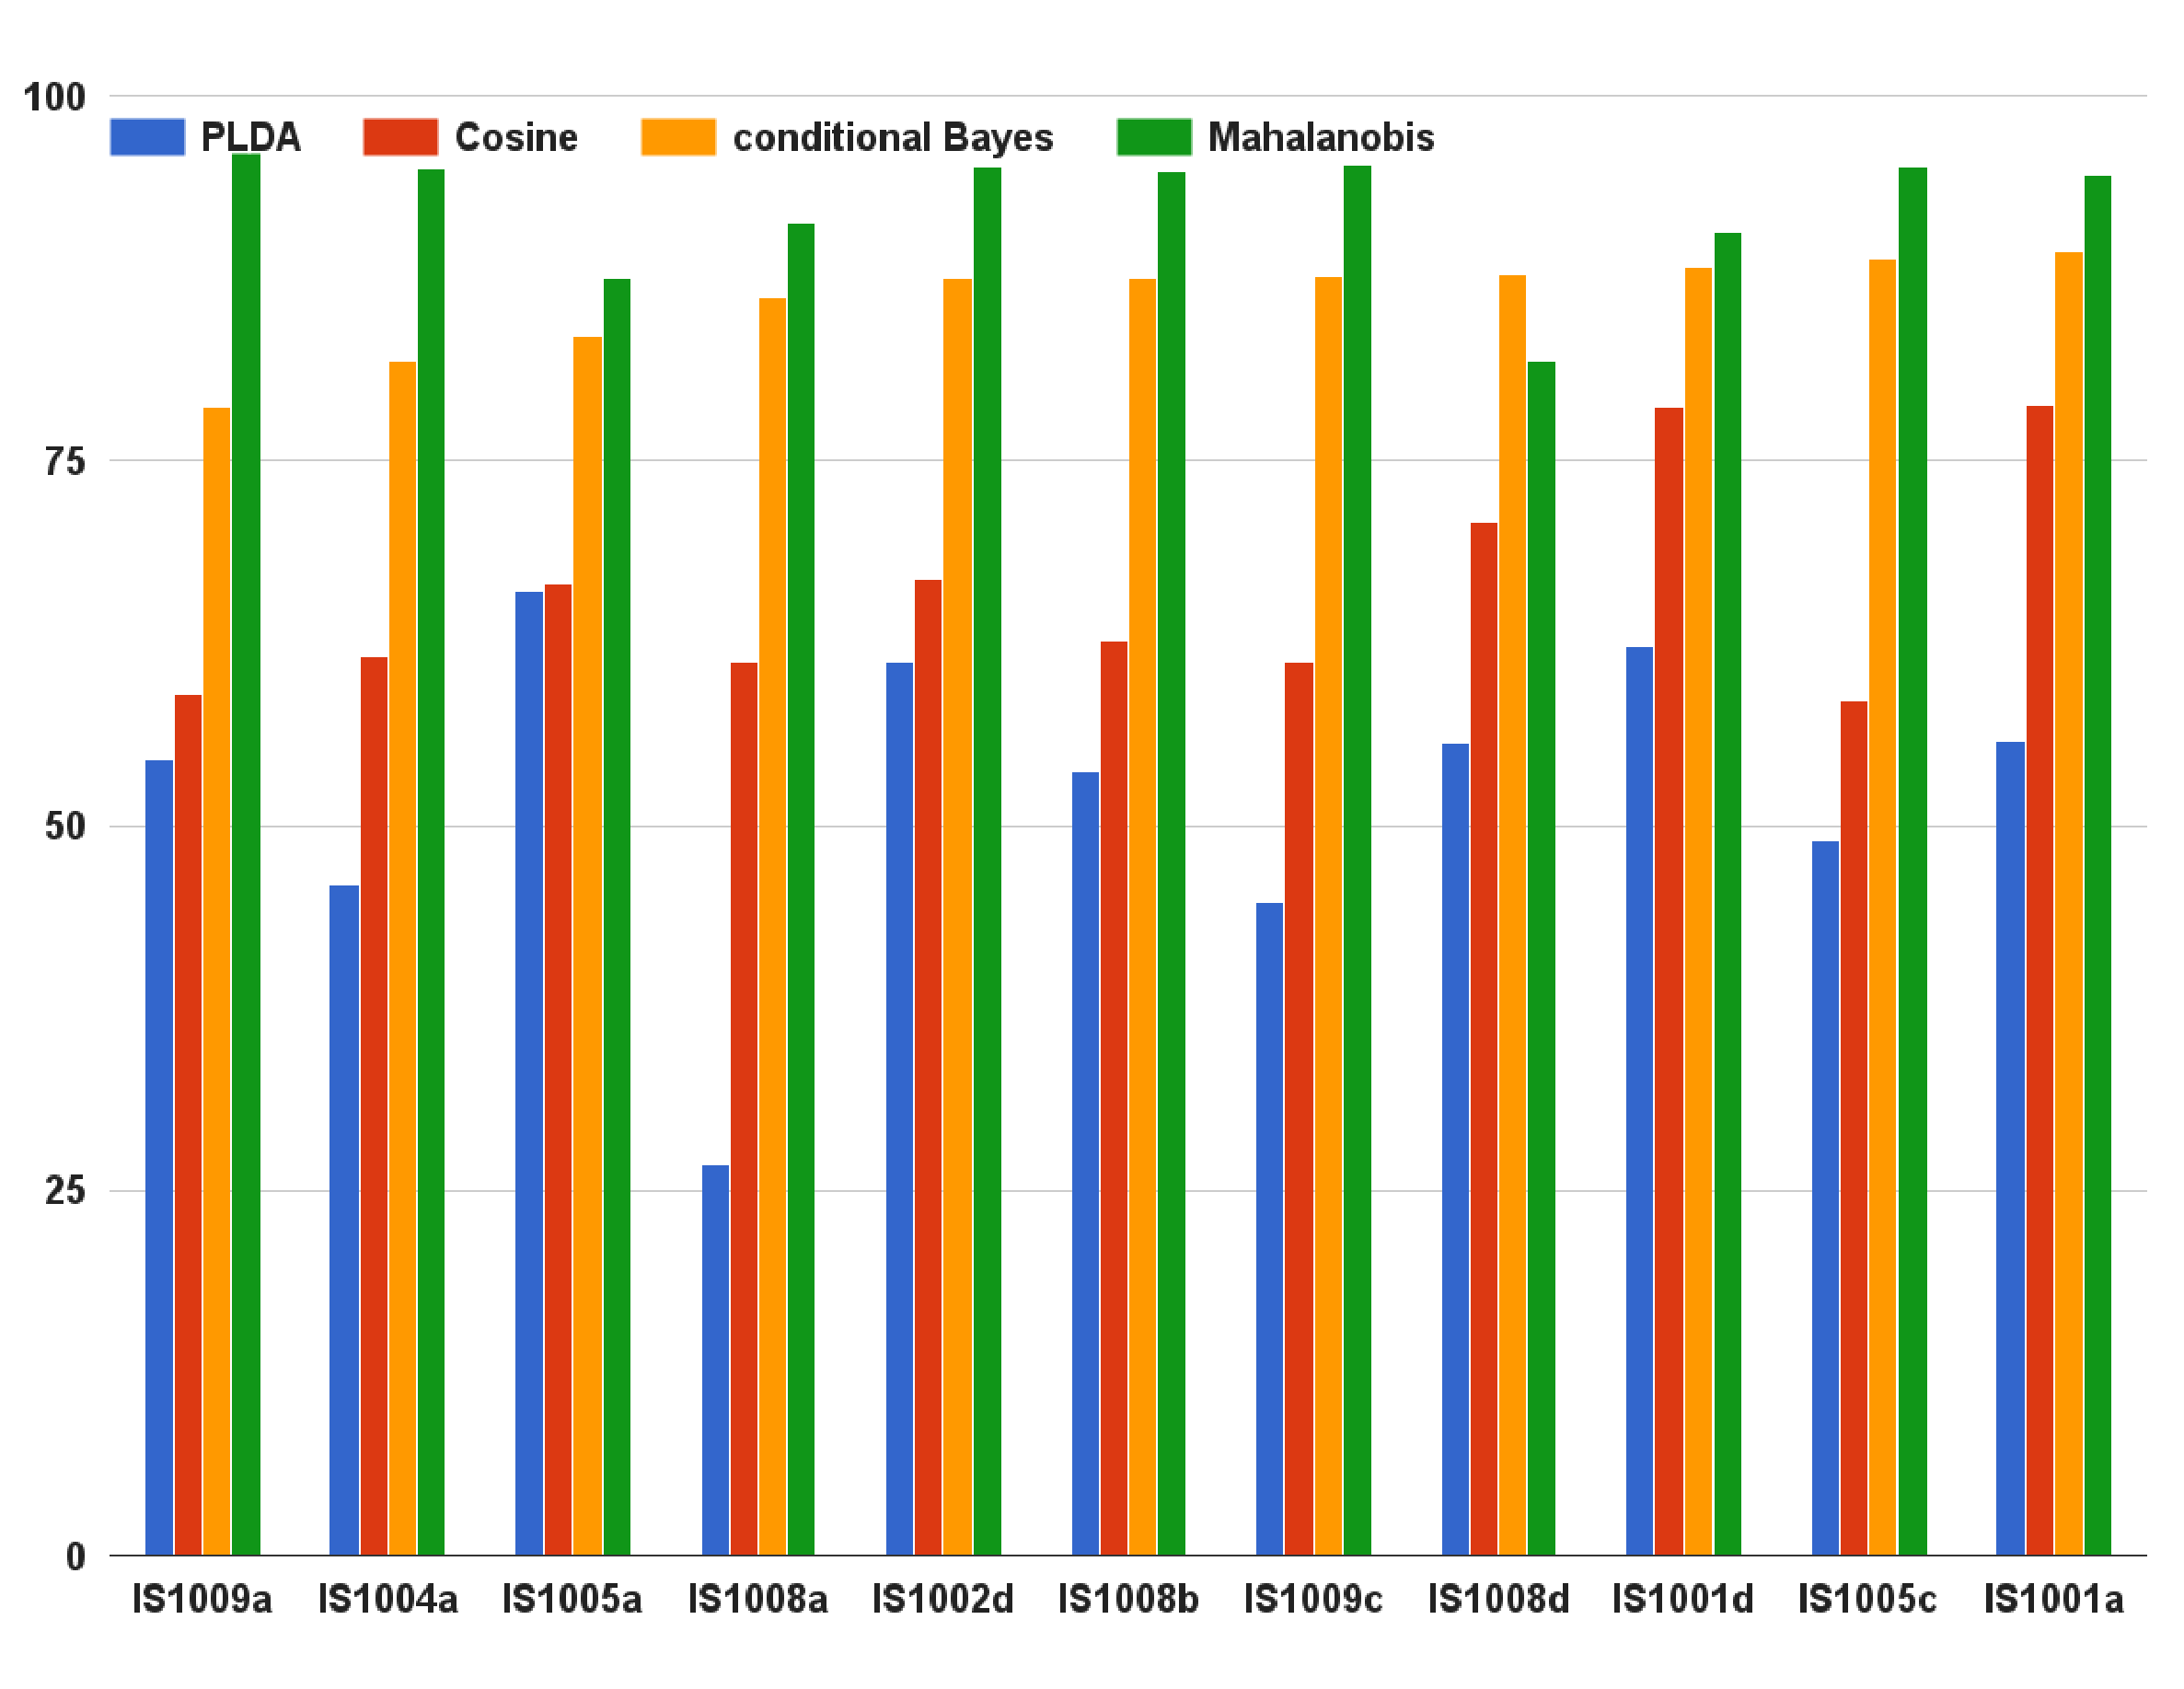
\includegraphics[height = 3.5in, width=1\textwidth]{figures/crssdiar_distances_der}
	\caption{ \small Comparison of diarization error rates calculated for different distance measures implemented in CRSS-SpkrDiar. DER is calculated for 11 AMI meetings (IS1009a-IS1001). Although absolute DER values have considerable room for improvement, it is clear that PLDA scoring significantly outperforms other distance measures.}
	\label{fig:ch5_compare_crssdiar_distances}
\end{figure}

This section briefly compares CRSS-SpkrDiar performance under the various distance measures described in Sect.~\ref{sec:plda_ilp}~and~\ref{sec:other_distances_ilp}. 
Experiments are conducted on AMI meeting data. 
Each meeting recording, referred to as a {\it session}, contains a minimum of 4 speakers. 
Other than the session audio file, no additional information is provided to the diarization system. 
However, as mentioned before some of the distance metrics, PLDA and conditional Bayers, require external data (i.e., development data). 
Development data is provided in the form of i-Vectors from NIST SRE challenges. 
For the purposes of these experiments i-Vectors were extracted for over 600 NIST SRE04,05,06 speakers. 
Multiple i-Vectors from different recordings were used for each speaker to provide sufficient channel variability. 
The PLDA model used here does not perform dimension reduction on the original 100-dimensional i-Vectors. 

Readers are advised not to examine Fig.~\ref{fig:ch5_compare_crssdiar_distances} based on absolute DER values. 
The purpose of this figure is to compare the performance of different distance measures presented in this chapter. 
The novel approach of using PLDA-based scores in ILP clustering significantly outperforms other distance measures. 
Figure~\ref{fig:ch5_compare_crssdiar_distances} also shows that conditional Bayes only slightly outperforms Mahalanobis distance. 
This observation is reasonable, since Mahalanobis and conditional Bayes essentially follow the same form and the difference is in the choice of covariance matrix. 

\section{Future Work}
\label{sec:chDiar_future}
As mentioned throughout this chapter, CRSS-SpkrDiar is a promising new research platform for speaker diarization. 
Every few weeks, we, the developers, receive requests for collaboration and questions about the state of the project from researchers around the globe. 
This chapter provided an outline of CRSS-SpkrDiar modules implemented so far. 
But as mentioned before, CRSS-SpkrDiar is a work in progress, both as a research platform and a means of achieving state-of-the-art speaker diarization performance. 
It was pointed out that speech activity detection and overlap detection modules are integrated into CRSS-SpkrDiar. 
A major improvement to CRSS-SpkrDiar would be to re-implement these components using Kaldi APIs, instead of using existing code in a plug-and-play manner. 
Finally, in addition to the two main components of speaker diarization, segmentation and clustering, some minor additions can help significantly improve performance. 
These additions include: alternative clustering algorithms, Viterbi resegmentation, and GMM-based speaker modeling. 
Considering the current state of CRSS-SpkrDiar and the reported error rates, provided sufficient time and effort, state-of-the-art diarization performance is well within our reach.


\section{Summary}
\label{sec:ch4_summary}
Chapter~\ref{chap:spkr_diar} introduced CRSS-SpkrDiar, a  speaker diarization system. 
The objective of CRSS-SpkrDiar is to create an all-encompassing research platform that supports state-of-the-art speaker and speech recognition, in addition to its primary objective, which is speaker diarization. 
This chapter focused on to main components of a speaker diarization system: 1) segmentation and 2) clustering. 
CRSS-SpkrDiar is considered a work in progress and further studies on this tool-kit are in development. 



\chapter{APPLICATIONS}
\label{chap:applications}

Previous chapters focused more on various technical aspects of co-channel speech and less on integrating the proposed techniques with other applications. 
This chapter highlights collaborative studies that address co-channel speech analysis for two problems: word-count estimation\footnote{Word-count estimation in co-channel speech is a collaboration between myself, Ali Ziaei, Abhijheet Sangwan, and my advisor Prof. John Hansen. At the time of the study, Ali Ziaei was a fellow PhD student at CRSS, Abhijeet Sangwan was (and currently still remains) a research professor in the department of Electrical Engineering at UT-Dallas.} and in-vehicle speech pertaining to driver safety systems\footnote{In-vehicle speech analysis studies are a collaboration with Amardeep Sathyanarayanan, Omid Sadjadi, and Prof. John Hansen. Amardeep and Omid were both PhD students at CRSS during the time of these studies.}. 
I consider these studies a driving force during my work as a PhD student, since research without outside stimulus can sometimes be mundane and out of touch. 
Collaborative studies, on the other hand, open up room for discussion and often lead to constructive feedback. 
Each of the studies presented in this chapter have led to major advancements in this dissertation. 

The contribution of this chapter is:
\begin{itemize}
	\item use overlap detection to improve word-count estimation in real environment noise conditions. 
	\item use overlap detection to predict competitiveness in conversations in in-vehicle speech analysis. 
\end{itemize}
Prior to the study on word-count-estimation, the main overlap detection algorithm developed for this dissertation was Gammatone sub-band frequency modulation (GSFM; see Sect.~\ref{sec:ch2_GSFM} in Chapter~\ref{chapter:front-end}). As we have learned, GSFM is highly susceptible to noisy conditions. 
This observation was made while evaluating overlapped speech detection in Prof-life-log data, a dataset with various types and amounts of noise~\cite{ziaei2013prof}. 
Pyknograms were the solution to a long-lasting effort of developing a robust overlap detection method for noisy conditions (see Sect.~\ref{sec:ch2_Pykno}~and~\ref{sec:ch2_Pykno_vs_GSFM} in Chapter~\ref{chapter:front-end}). 

In-vehicle speech analysis contributed to a significant novelty in this dissertation's perspective in addressing co-channel speech (in terms of distinguishing co-channel speech from overlap). 
Prior to the collaborative study on in-vehicle speech, the sole focus of this dissertation was on examining overlapped speech. 
It was during this project that the importance of other conversational traits, such as turn-takings and speaker response time, became more visible and prompted further investigation. 

The remainder of this chapter provides a brief description of word-count estimation, Sect.~\ref{sec:wce_cch}, and in-vehicle driver safety systems, Sect.~\ref{sec:invehicle}. 


\section{Word-Count Estimation in Co-channel Speech}
\label{sec:wce_cch}
The ability to estimate the number of words spoken by an individual over a certain period of time is valuable in second language acquisition, health-care, and assessing language development. 
Word-count values are also useful in the analysis of massive audio data, such as the Prof-life-log corpus~\cite{ziaei2013prof}. 
Prof-life-log is a speech corpus that contains long durations of audio recordings. In this collection, the primary speaker wears a portable LENA recording device~\cite{lena_device} throughout a work day. 
Although the primary speaker is always the same individual, he frequently interacts with different people. 
An estimate of the primary speaker's speech activity (i.e. word-count) facilitates analyses that predict the level of productivity and helps determine areas in the recording that are more ``valuable'' for further processing. 
The proposed word-count estimator in this study is tested on long duration files from the Prof-Life-Log corpus. 

Establishing a robust automatic framework to achieve high accuracy is non-trivial in realistic scenarios due to various factors such as different conversation styles or types of noise that appear in audio recordings, especially in multi-party conversations (i.e., co-channel speech). 
This section proposes to use overlap detection to estimate the likelihood of overlapping speech in a given audio file in the presence of environment noise. 
The resulting overlap information is embedded into a word-count estimator, which uses a linear minimum mean square estimator (LMMSE) to predict the number of words from syllable rates, which are easier to detect using only acoustic information. 
Figure~\ref{fig:wce_system_overview} shows an overview of the proposed word-count estimator. 
The overlap detection system acts as an augmented module in the system, similarly to how speech activity detection removes silence for the word-count estimation (WCE) system. 

\begin{figure}[t!]
	\centering
	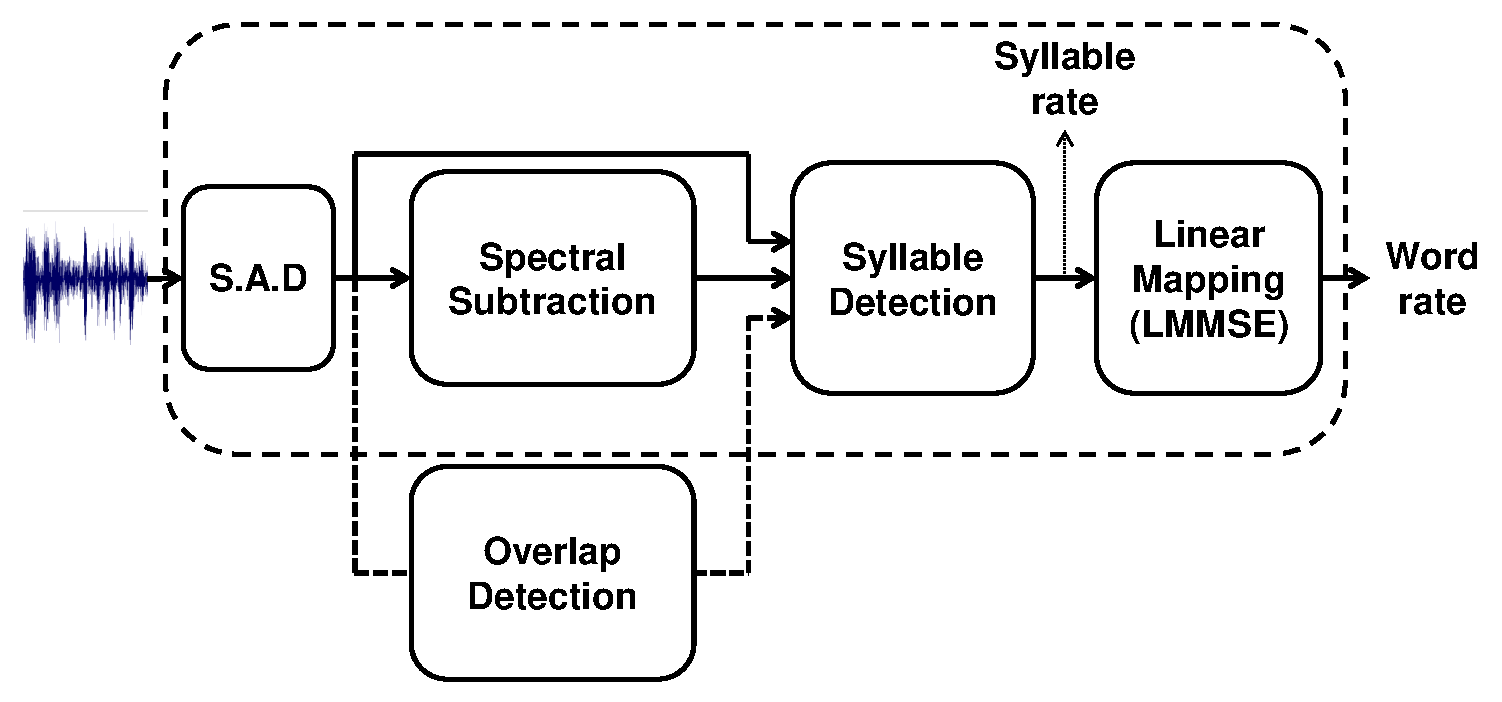
\includegraphics[height = 2.8in, width=1\textwidth]{figures/wce_ovl_SLT2014_systemconfig_figur-crop}
	\vspace{-3mm}
	\caption{Word-count estimation system configuration. The overlap detection system is shown as an addition to the original system.}
	\label{fig:wce_system_overview}
\end{figure}

\subsection{Word-count estimation}
\label{sec:wce}
The word-count estimator is adopted from previous studies~\cite{IS14_wce}, which estimate the number of words per unit time by applying a linear transformation to the syllable rate. 
Syllable rates are calculated based on a modified version of the {\it mrate} algorithm~\cite{Wang_slbl} using acoustic characteristics of the signal: pitch, smoothed spectrogram. 
This algorithm detects the location of syllables in a given speech segment. 
The number of detected syllables per unit time are used to calculate syllable rates throughout the audio. 
As~\cite{IS14_wce} show, the help of alinear minimum mean square estimator (LMMSE) can generate linear coefficients that map syllable rates to the number of words per unit time, as shown below: 
\begin{equation}
\label{eq:lmmse_wce}
{\tilde {\bf a}} = argmin_{\bf a} \Big\{\frac{1}{N}\sum_{\bf a}\big(W_r(n)-{\bf a}S_r(n)\big)^2\Big\},
\vspace{-1mm}
\end{equation}
where $W_r(.)$ and $S_r(.)$ are the word-count and syllable rates at any given time, respectively. 
$n$ indicates the index of a given time segment and $N$ is the total number of segments used to train the linear transformation parameter, ${\tilde {\bf a}}$. 
The transformation parameter, ${\tilde {\bf a}}$, is a vector comprised of a bias factor and a linear coefficient. 
In cases where the bias factor is non-zero, $S_r(n)$ is replaced by $\big[S_r(n) \hspace{2mm} 1\big]^T$. 
The linear transformation parameter(s) can be trained using manually transcribed background conversational data. 
For this study, we rely on a subset of Prof-Life-Log data that has been transcribed for word-counts. 

In~\cite{IS14_wce}, higher accuracy is obtained by introducing speech activity detection (SAD)~\cite{sadjadi2013unsupervised} and spectral subtraction to the front-end of the WCE. 
SAD reduces false-alarms by omitting non-speech regions, a decrease which helps avoid detection errors made by the syllable detector. 
Spectral subtraction enhances speech regions~\cite{boll1979spectralSubtraction}, allowing the syllable detector to identify voiced regions more accurately. 
None of these techniques, however, are able to address the issue of overlapped speech. 
Therefore, the novelty in this study is to use overlap detection as an additional layer of data pruning to reduce false alarms. 

An estimation of the location and amount of overlapped speech in a given speech segment can be combined with SAD labels to supply an additional layer of data pruning before syllable detection. 
Overlap detection is fed to the syllable detector as additional information (see Fig.~\ref{fig:wce_system_overview}).  
First, SAD is performed on the raw data to detect speech locations. 
From SAD labels, non-speech regions are used to estimate the noise level in each short segment and submitted to the spectral subtraction algorithm. 
Speech-only segments are passed to the syllable detector after applying spectral subtraction. 
Finally, syllable rates (calculated by dividing the number of syllables by the segment length) are transformed into word-count rates using LMMSE coefficients. 
In our proposed system, overlap detection outputs are combined with SAD results, to provide an extra layer of data pruning. 

The overlap detection algorithm used in this framework is based on Pyknograms, which are described in Chapter~\ref{chapter:front-end}. 
Pyknograms were chosen here as a robust solution to the highly noisy data in Prof-life-log. 
In Pyknograms, non-resonant speech is emphasized over background noise and unvoiced speech. 
This allows improved performance in noisy conditions, while simultaneously improving syllable detection, due to the high correlation between voiced speech and syllables. 

\begin{table}[b!]
	\centering
	\renewcommand{\tabcolsep}{2.5 mm}
	\renewcommand{\arraystretch}{1.3}
	\vspace{0mm}
	%\vspace{1mm}
	\caption {WCE performance in Prof-Life-Log with respect to overlapped speech.}
	\label{tab:wce_ovl}
	\vspace{2mm}
	\begin{tabular}{p{0.8cm}*{6}{c}}
		\bf $\frac{minimum\hspace{1mm} mean \hspace{1mm} square \hspace{1mm} Error}{\# of words}$\\ \hline \hline
		overlaps & NOT&\hspace{-7mm}removed	&  &     &    5.71\% \\ 
		overlaps&\hspace{1mm} removed	&		&	&     &    \bf3.69\% \\ \hline
	\end{tabular}
	\vspace{-1mm}
\end{table} 

Word rates are extracted from 5 days of prof-life-log recordings. 
Each day contains roughly 6 to 8 hours of audio, labeled to include the transcriptions of the primary speaker's speech, speaker labels (primary vs. secondary), and the type of environment in which the recordings take place. 
We have mostly concentrated on environments that are more likely to contain overlapped speech, such as multi-party meetings and conferences.
The sampling frequency from the LENA device is $44.1kHz$, which we have down-sampled to $8kHz$. Table~\ref{tab:wce_ovl} shows over $35\%$ improvement in relative mean square error after removing overlapped regions. 


\newpage
\section{In-vehicle Conversation Analysis}
\label{sec:invehicle}
Many in-vehicle conversations are beneficial in keeping drivers alert and active, however there are also instances where a competitive conversation may adversely influence driving performance. 
Identifying such scenarios can improve vehicle safety systems by fusing the knowledge obtained from conversational speech analysis and vehicle dynamic signals. 
This section briefly describes how smart portable devices can be incorporated to create a unified platform and record in-vehicle speech as well as vehicle dynamic signals required to evaluate driving performance. 
This study shows that turn-takings and overlapped speech segments, as conversational speech cues, under certain conditions deviate from normal driving patterns. 

Auditory based distraction caused by in-vehicle conversations is difficult to investigate. The main issue being that not all speech activity is considered distractive to drivers. 
The study in \cite{ESPA} used speech activity detection to track the impact of any speech activity on driving performance. 
The conclusion being that although some impact is observed, driving performance is highly affected by the type of conversation. 
In this study, we further investigate the possible consequences of drivers' involvement in \emph{competitive} conversations while driving. 
It is expected that active engagement conversations results in deviations from usual driving patterns, which are identified through the analysis of different driving maneuvers. 

\subsection{System Description}
\label{sec:system_description}
\vspace{3mm}
Performing certain secondary tasks while driving is likely to adherently impact driving performance. 
Some tasks are inevitable or difficult to restrict, such as controlling the navigation system. 
However, other secondary tasks such as engaging in a conversation with other passengers or cell-phone conversations can be controlled if they are determined to compromise driving performance. 
This sections shows a feedback system which not only evaluates variations in driving performance but also helps mitigate the influence of in-vehicle speech if it is found to adversely influencing the driving performance (see Figure~\ref{fig:system_description_fig}). 
There are two separate subsystems in the proposed framework. 
The first subsystem evaluates the driving performance by identifying maneuvers and then comparing them with the driver's regular driving patterns. 
If a maneuver is recognized as ``abnormal'', the driver's in-vehicle speech involvement is monitored to see whether that is the cause for unusual driving behavior. 

\begin{figure}[h]	
	\centering
	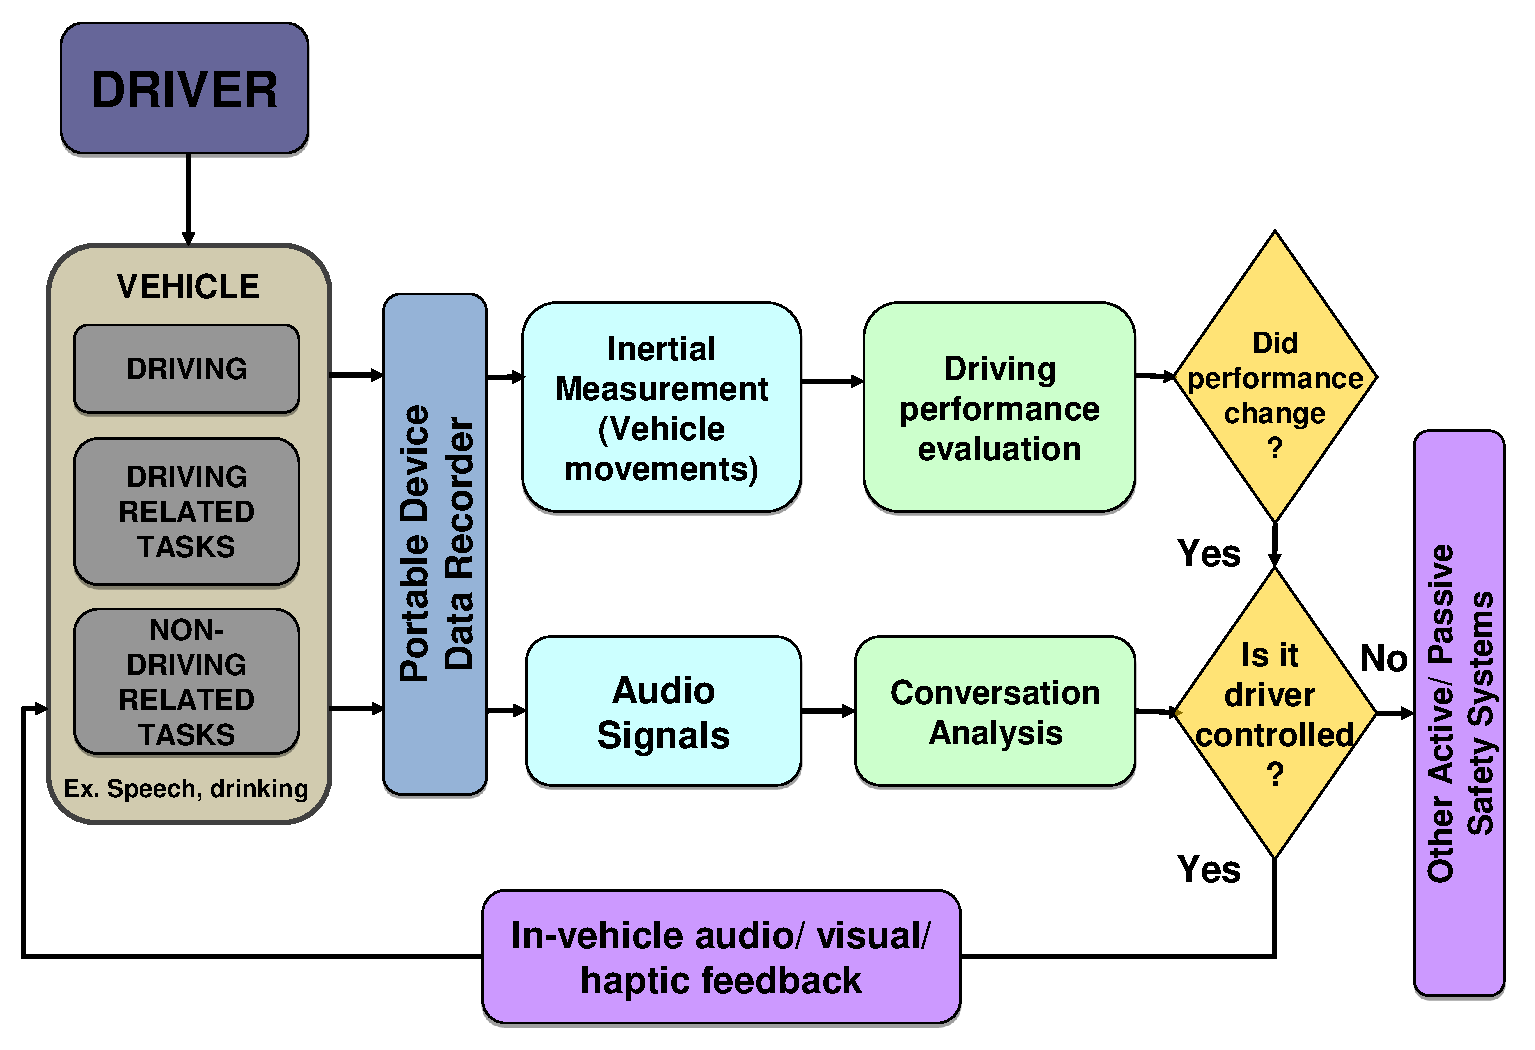
\includegraphics[width=\linewidth]{figures/system_description-crop}
	\caption {System description}
	\label{fig:system_description_fig}
\end{figure}

The second subsystem evaluates the driver's involvement in conversations. 
An addition to previous studies on in-vehicle speech~\cite{ESPA} is that rather than considering any in-vehicle speech activity, the emphasis here is on the driver's involvement in conversations. 
This involvement is analyzed by measuring the amount of overlapped speech segments as well as turn-taking rates during conversations. 
One of our objectives was to demonstrate that these two metrics are reliable indicators of the driver's focus on speaking as opposed to the primary task, which is driving. 
If in-vehicle speech activity is identified to adversely impact the driver's performance, it can be controlled passively by providing an initial warning feedback to the driver and/or co-passengers to halt the conversation until the vehicle state returns back to normal. 
Monitoring driving performance continues and any secondary tasks performed by the driver, other than those essential to driving, could be sequentially cut off. 
The uniqueness of this system is the ability to identify driving performance variations and isolate the source of distraction. 

The technical details of the driving evaluation system falls beyond the scope of this dissertation. 
For the curious reader, it suffices to know that performance is measured by statistically modeling driving maneuvers using vehicle dynamic signals (e.g., steering wheel angle, speed, acceleration)~\cite{sathyanarayana2013belt}. 
Maneuvers form the basic building blocks of driving routes, hence analyzing them can be employed as a key component in understanding driving performance. 
Variations in driving performance can be recorded by observing how each maneuver is executed and comparing the characteristics of maneuvers that fall under the same category. 

\subsection{Conversation Analysis}
\label{sec:conversation_analysis}
As mentioned in Section~\ref{sec:system_description}, the purpose of utilizing audio data is to analyze the conversation taken place in the vehicle and determine whether it is causing driver distraction. 
We speculate that the level of competitiveness in a conversation should correlate with driving performance. 
In order to measure competitiveness in a conversation, two features are utilized. 
The first is the turn-taking rate. 
An increase in the number of turn takings per time unit can imply that speakers are taking interest in the conversation. 
Additionally, the amount of overlapped speech is considered a potential competitiveness feature~\cite{Schegloff}. 

By now the readers are likely familiar with overlap detection algorithms, but turn-taking has not been covered in this thesis. 
Although there are more sophisticated ways of estimating turn-takings rates in a conversation (using speaker diarization). 
This study uses speech activity detection (SAD) to detect start and end-points of active speech regions in a conversation. 
The start-points are labeled as the triggering points of a turn in the conversation. 
Since this definition for turn taking may not always imply that both speakers are involved in a conversation, for example in instances when one of the speakers pauses in between sentences, the amount of overlapped speech in regions with a high turn taking rate is used to assure that both speakers are involved. 


\vspace{3mm}
\section{Data Description}
\label{sec:data_description}
Since this study focuses on understanding the influence of in-vehicle speech on the driver, care should be taken to minimize influence from other modalities on the driver.  
An experimental setup was conducted that allowed drivers operate the UTDrive vehicle under real-traffic conditions~\cite{pongtep2007utdrive}. 
The data was collected under similar weather and traffic conditions for all drivers and the route consisted of residential areas and highways and took place in an average of twenty minutes per session. 
In the past few years, the research community has shown an increasing interest in using portable devices (sensor loaded smartphones and tablets) to instrument a vehicle and use it as a pseudo-data collection platform. 
It has also been shown that using sensor data from these portable devices yields to comparable results in maneuver recognition CAN-bus signals obtained from instrumented vehicles~\cite{sathyanarayanaITSC2012,sathyanarayanaSAE2013}. 
In this study, data was collected in the UTDrive instrumented vehicle (UTDrive) along with the portable device mounted in the car \cite{sathyanarayanaITSC2012}. However, only the sensor information from the portable device has been used for the entire analysis.
Using a 10.1" Samsung Galaxy Tablet and an Android OS as the portable device platform, an Android application has been developed to collect all the available sensor information on the device synchronously. 
The available sensors and derived information include a camera, microphone, accelerometer, gyroscope, magnetometer, orientation, compass and GPS signals. 
A detailed description of the UTDrive App for portable device and the sensor information can be found in\cite{sathyanarayanaITSC2012}. 


Data were designed with the intention to create competitive behavior in the driver. 
Drivers were asked to perform tasks, which activate their competitiveness and involvement in order to increase the amount of overlapped speech~\cite{Schegloff} and turn-takings. 
However, the fact that the purpose of the study was to collect competitive conversations was hidden from the drivers to avoid self-consciousness. 
The driving route was divided into four segments, repeated in two phases. 
In the first phase, the driver drives through the complete route without performing any secondary task to become familiar with the route and the vehicle. 
In the second phase the driver is asked to perform a different task in each segment of the route. 
Four different tasks are chosen to include as many variations of conversational speech as possible. 
The tasks are described below:

\begin{figure}[h!]
	%\vspace{-5mm}
	\centering
	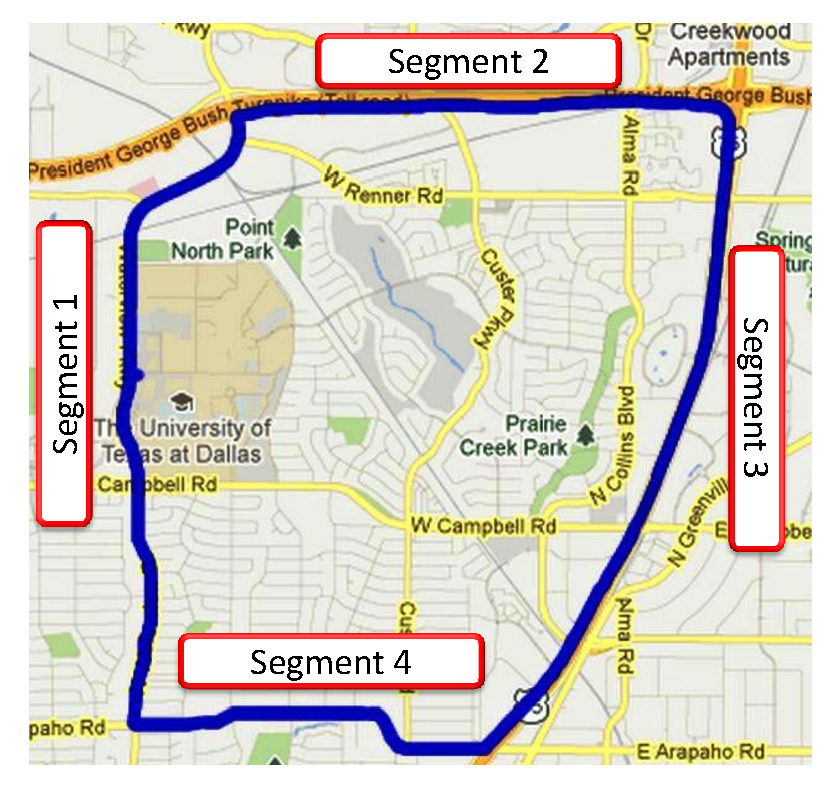
\includegraphics[width=0.6\linewidth]{figures/route_map-crop}
	\caption {Driving route with different conversational task segments.}
	\label{fig:map}
	%\vspace{-5mm}
\end{figure}

\begin{itemize}
	
	\item Segment 1: At the beginning, in order to “break the ice” the passengers will initiate a simple conversation by asking the driver questions about casual topics such as the weather (Other topics may be chosen).
	\item Segment 2: In this segment one of the passengers picks an object and the driver and the other passenger are supposed to guess the object using the hints provided to them. Whoever guesses first is the winner. This game is chosen to increase turn-taking and overlapping speech segments.
	\item Segment 3: A set of TIMIT sentences are played through a portable tablet and the driver is required to repeat each sentence before the next sentence is played.
	\item Segment 4: An argument is initiated by one of the passengers. This second conversation is more involved compared to that in segment 1. The difference here is that the driver’s opinion on a debatable topic is asked and based on his/her answer, the passengers take the other side and try to argue on the subject.
	Each of the tasks described above takes place on one of the legs in the route as labeled on the map in Figure~\ref{fig:map}.
	
\end{itemize}




\subsection{Experimental results}
An advantage of this experimental setup over previous studies~\cite{sathyanarayanaITSC2012, sathyanarayanaSAE2013,ESPA} is that both the in-vehicle speech data and the data required for maneuver recognition are recorded by the portable device. 
This results in a more concise and cost effective data acquisition platform.

Statistical information from the inertial measurement sensors such as accelerometer and gyroscope of the portable device were extracted on a per frame basis (once per second). 
Statistical information such as maximum lateral acceleration, mean of the vehicle speed, variance of yaw-gyroscope (refer to \cite{sathyanarayanaITSC2012} for a detailed list) form the dominant feature space used in training the maneuver specific models. 
Using Support Vector Machines (SVM), the maneuver segments are recognized and classified with a high average accuracy of over $90\%$. 
Once classified, driving performance is evaluated for each maneuver according to its class. 
Thresholds are appropriately set in the feature space to identify any abnormal or risky driving patters. 
Examples of the driving performance evaluation is shown in Figure~\ref{fig:driving_performance}. 
This figure compares a drivers performance on the same route with and without the stimulus of competitive conversations. 
The regions marked green are locations where the driver drove similar to his usual driving pattern. Yellow regions correspond to where the driver showed slight variations in the driving pattern. 
The red regions are locations where the driver executed an abnormal or risky maneuver. 
All regions concur with the visual and perceptual verification obtained by looking at the video from the data recordings. 

\begin{figure*}[h!]
	%\vspace{-5mm}
	\centering
	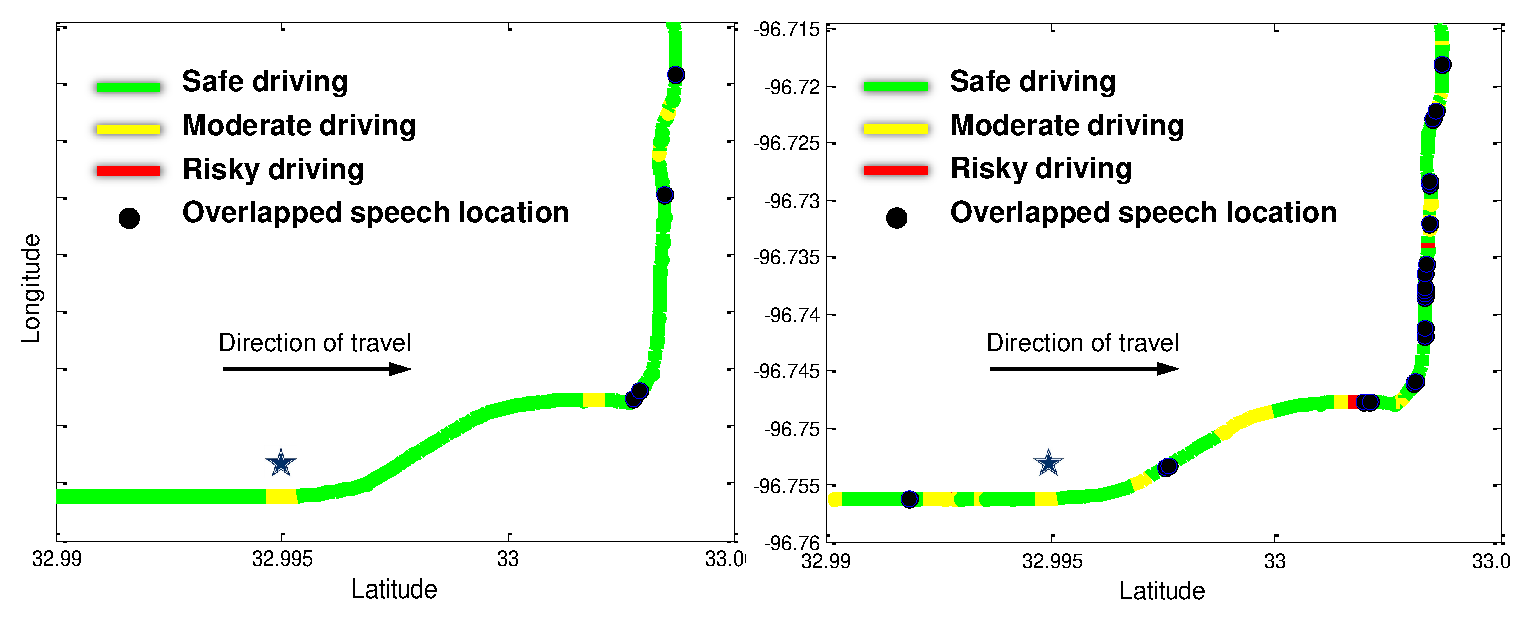
\includegraphics[scale=0.6]{figures/driving_and_overlap}
	\vspace{-5mm}
	\caption {Driving performance evaluation on a section of the route in two phases. Left (phase 1)-  performance with minimal conversations. Right (phase 2)- performance drop as a result of the increase in the amount of overlapping speech.}
	\label{fig:driving_performance}
	\vspace{-5mm}
	%\vspace{-5mm}
\end{figure*}


As Figure~\ref{fig:driving_performance} suggests, there are some instances in the route where no direct relationship is observed between overlapped speech and performance-drop, see the area marked by a star in the figure. 
This was expected, since there are always other sources that can cause irregularities in the driver's maneuver execution patterns. 
Hence, speech related features should be analyzed in more detail to confirm that the conversation is the source of distraction. 
With this intention, the patterns of turn-takings and overlapped speech segments were jointly investigated over time. 
Turn-taking and overlapped speech rates are defined as below:
\begin{equation}
ovl_{rate} = \dfrac{\textrm{Number\: of\: overlapped\: samples\: in\: window}}{\textrm{window\: length}} \nonumber
\end{equation}
\begin{equation}
tt_{rate} = \dfrac{\textrm{Number\: of\: turntakings\: in\: window}}{\textrm{window\: length}} \nonumber
\end{equation}

Figure~\ref{fig:turntaking_and_overlap} depicts the average turn-taking and overlapped speech rate in conversations before observing significant drop in driving performance. 
Each plot belongs to a different scenario. 

\begin{figure*}[h!]
	\vspace{-5mm}
	\centering
	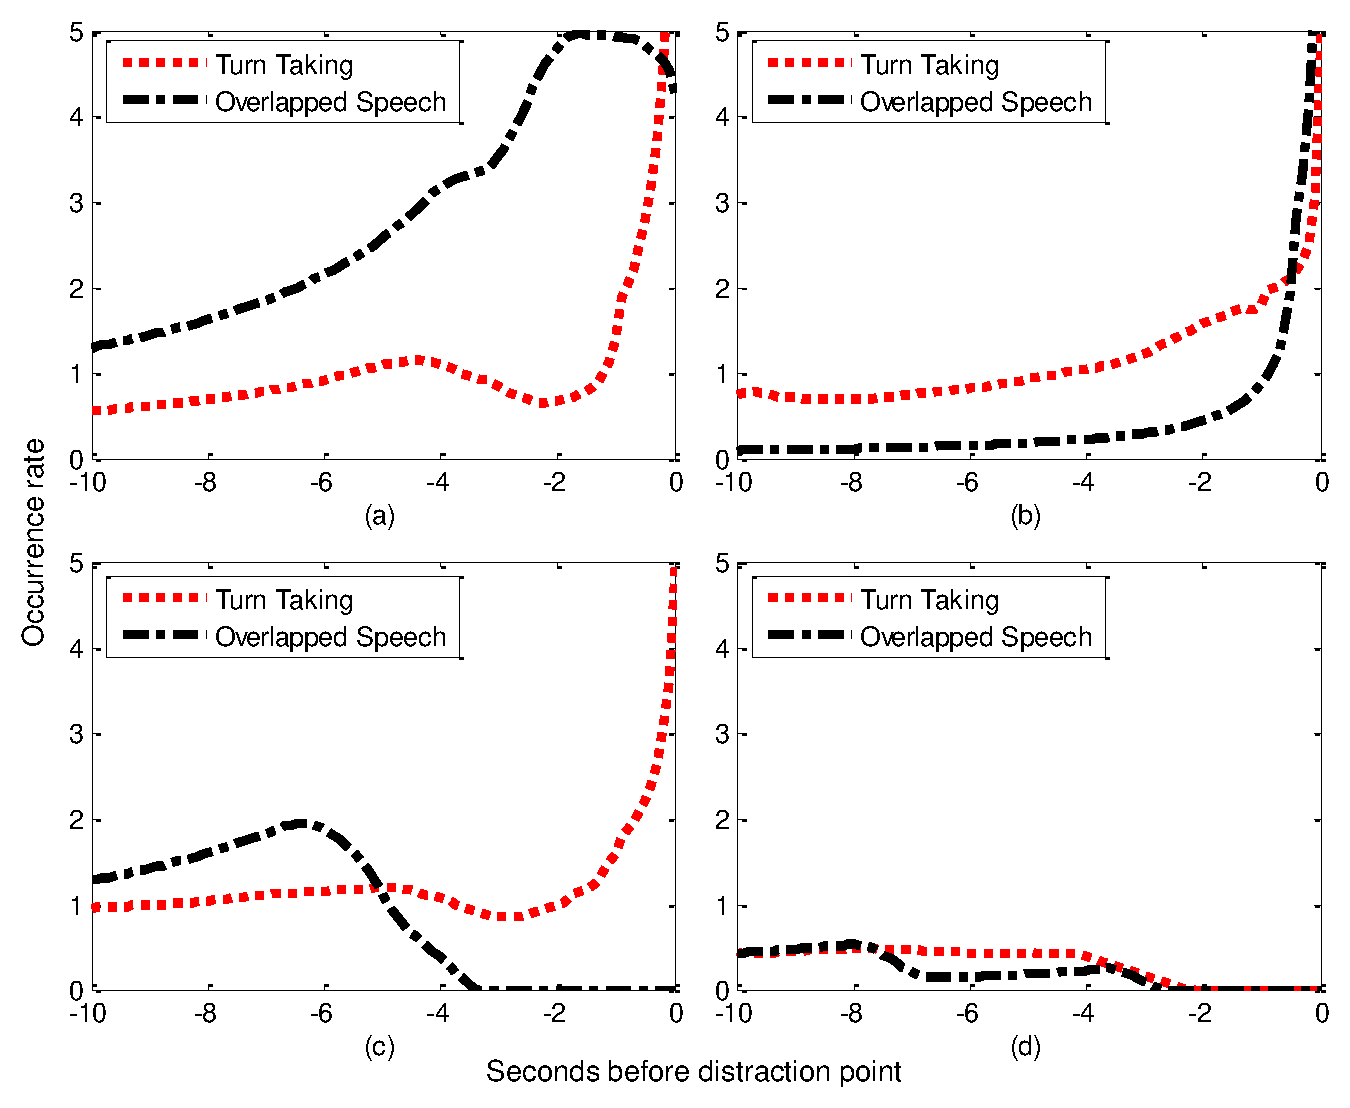
\includegraphics[scale=0.5]{figures/ttr_and_ovl}
	\caption {Turn-taking and overlapping speech rate before observing the first major drop in performance in different scenarios.}
	\label{fig:turntaking_and_overlap} 
	%\vspace{-5mm}
\end{figure*}

\newpage
If both the turn-taking and overlapped speech rates increase before the performance drops, the conversation can be a potential source of distraction. 
Figures~\ref{fig:turntaking_and_overlap}-a and b are more interesting, since both features increase with time. 
Figure~\ref{fig:turntaking_and_overlap}-c was also observed in our experiments, where the overlapped speech rate increases and goes back to $0$ per second before driving performance drops. 
Figure~\ref{fig:turntaking_and_overlap}-d shows an instance where turn-taking and overlapped speech rate significantly drop prior to any changes are observed in driving performance, lowering the possibility that the conversation being the source of distraction. 

\newpage
\section{Summary}
\label{sec:ch4_summary}
The final chapter highlights a selection of collaborative studies between co-channel speech analysis and other signal processing applications. 
The content was presented in the form of an applications chapter. 
The first section describes how overlap detection can be integrated into a word-count estimation system to reduce false-alarm errors in detecting syllables. 
The second section uses co-channel speech analysis, namely turn-taking rate estimation and overlap detection, to measure speakers' attentiveness in conversations. 
The predicted ``attentive'' is used in a driver safety system to identify in-vehicle conversations that jeopardize driver and passenger safety. 


\chapter{CONCLUSIONS}

This study presented a detailed description of co-channel speech analysis in the context of speaker recognition. 
As repeatedly mentioned throughout the course of this thesis, co-channel speech refers to single-channel audio signals with more than one speaker. 
Great care was taken to highlight the difference between overlap and co-channel speech. 
While co-channel refers to any signal with more than one speaker, overlap refers to parts of co-channel audio where more than one speaker is speaking. 
The distinction between overlap and co-channel is the first contribution of this thesis. 
Although this contribution may appear trivial at first glance, it was shown that the majority of co-channel research considers overlap synonymous to co-channel speech, a misconception that reduces the applicability of some attempts to compensate overlapped speech in speaker recognition. 
In other words, addressing overlap in co-channel speech is not sufficient for a large class of speaker recognition problems. 
This narrative is carried out throughout the first few investigations of this study. 

The study considers the impact of overlapped speech on speaker recognition performance. 
Speaker recognition is typically manifested through speaker verification experiments. 
It was shown that replacing single-speaker audio data with overlapped data reduces verification performance to up to one order of magnitude. 
For example, equal error rates increase from 1.5\% for single-speaker audio from the GRID corpus to approximately 23\% for overlapped data (depending on the nominal signal-to-interference ratio). 
This observation shows the legitimacy of past studies in prioritizing overlap relative to other forms of co-channel data. 
The traditional approach to deal with such drastic performance drop is to measure/detect overlapped segments in speaker recognition experiments. 
Therefore, the second stage of this study provides an extensive investigation of overlap detection methods. 

Overlap detection provides a unique perspective in highlighting the differences between single-speaker and overlapped speech. 
The algorithms proposed in this study focus on the harmonic structure of speech. 
Speech harmonics have traditionally been used as a way to identify overlapped speech. 
The fact that speaker recognition is highly influenced by voiced speech further motivates this approach. 
Harmonics are an important component of voiced speech and therefore, harmonic based analyses of overlapped speech fits well with the theme of this study. 
The two methods proposed for overlap detection are: 1) Pyknograms and 2) Gammatone sub-band frequency modulation (GSFM). 
Pyknogram extraction is a 2 step process of obtaining a binary mask for time-frequency units corresponding to the amplitude spectrogram. 
Frequencies across the spectrogram are first estimated using the Teager Energy Operator (step 1). 
The estimated frequencies are then pruned to only include prominent resonances (step 2). 
Pyknograms provide two important features that are useful for overlap detection: 1) unlike many existing speech representations, Pyknograms do not depend on the number of speakers; 2) Pyknograms are effective in suppressing non-harmonic speech, which provides robust performance in noisy conditions. 
In addition to Pyknograms, GSFM was also proposed as a way to magnify the presence of multiple harmonics in time-frequency units. 
GSFM incorporates the non-linearity of sinusoidal frequency modulation to obtain frequency modulation spectra. 
The relative roll-off of FM spectra is then used to summarize the information in each time-frequency unit. 
Evaluations show that although in controlled conditions GSFM outperforms Pyknograms for overlap detection, under noisy conditions Pyknograms are significantly more reliable. 

In addition to introducing overlap detection methods, a novel technique is proposed that uses overlap detection decisions as quality measures for speaker recognition experiments. 
Using overlap detection as quality measures (aka meta-data) is more desirable compared to the traditional approach, which is to detect and remove overlapped segments. 
The advantage of quality measures is in the fact that not all overlapped speech should be thrown away, especially with limited data. 
The algorithm used to fuse quality measures with speaker recognition decisions is called Q-stack, which concatenates multiple scores and summarizes the final speaker verification decision using support vector machine (SVM) certainties. 
Fusing overlap meta-data with speaker verification scores relatively reduces speaker verification error rates by approximately 20\%. 

The study also focused on evaluating speaker recognition performance in co-channel speech. 
It was shown that although overlap is damaging to speaker recognition performance, the impact of co-channel is much more significant. 
In the case of Switchboard2 telephone conversations, the impact due to non-overlapping co-channel speech is over 18\% absolute increase in EER (single-speaker performance is 5\%). 
Meanwhile, the increase in EER due to overlapped speech is slightly over 2\%. 
This puts the impact of overlap vs. co-channel speech in perspective for real conversational speech. 
In an effort to compensate co-channel in realistic speaker recognition probelms, a standard i-vector/PLDA system was evaluated. 
Many approaches were investigated to improve probabilistic linear discriminant analysis (PLDA) for co-channel speech. 
1) One method was to add co-channel data to PLDA training, called mixed PLDA. 
Mixed PLDA was presented to treat speaker interference in the same manner PLDA addresses channel mismatch.
2) A second method was dual-eigenvoice PLDA (dePLDA). dePLDA uses two identical eigenvoice matrices to model within- and between-speaker variability. The difference between dePLDA and standard PLDA is in replacing the eigen-channel matrix with a second eigen-voice. 
3) The study also introduced co-channel aware PLDA (caPLDA), which proposed alternative formulations to PLDA for speaker recognition in co-channel speech. 
These alternative formulations replace within-speaker variability with a linear combination of between- and within-speaker covariances. 
Different coefficients are investigated in the proposed linear combination framework. 
Results show that although some performance improvement is obtained by the proposed caPLDA. 
dePLDA on the other provides significant improvement over mixedPLDA and standard PLDA.  

A speaker diarization research platform is presented in this study, called CRSS-SpkrDiar. 
Speaker diarization addresses the problem of ``who spoke when?'', which is a relevant question for co-channel signals. 
Therefore, diarization is considered an important aspect of speaker recognition in co-channel speech. 
In a sense, most of this thesis considered speaker recognition over entire co-channel signals, while speaker diarization addresses speaker recognition within a co-channel signal. 
CRSS-SpkrDiar is a C++ library that includes the implementation of state-of-the-art speaker diarization techniques. 
This study presents the main components of CRSS-SpkrDiar while providing sufficient details related to speaker diarization in general. 
CRSS-SpkrDiar is considered a major contribution of this comprehensive study on co-channel speech and is presented as a stepping stone for future work. 






\chapter{Appendix: i-Vector/PLDA speaker recognition}
\label{appendix:ivector_plda_spkr_id}
This appendix is presented for the curious reader who is interested in becoming more familiar with the i-Vector/PLDA speaker recognition platform. 
This is in no means a comprehensive introduction for this type of system, rather its function is to provide context for proposed systems in Chapter~\ref{chapter:backend}. 
Speaker recognition in i-Vector/PLDA system is implemented in a way to fall in the speaker verification framework. 
Much like a GMM-UBM system, each decision provides a likelihood ratio verifying whether a train speaker matches audio from a test speaker. 
An i-Vector/PLDA system typically trains a speaker model (i.e., i-Vector) using multiple training files. 
Unlike GMM-UBM, test speakers are also represented by speaker models. 
Therefore, train and test speakers are treated similarly in an i-Vector/PLDA system. 
Figure~\ref{fig:ivector_plda} summarizes a typical i-Vector/PLDA system~\cite{dehak2011front}. 

\begin{figure}[h!]
	\centering
	\vspace{0mm} 
	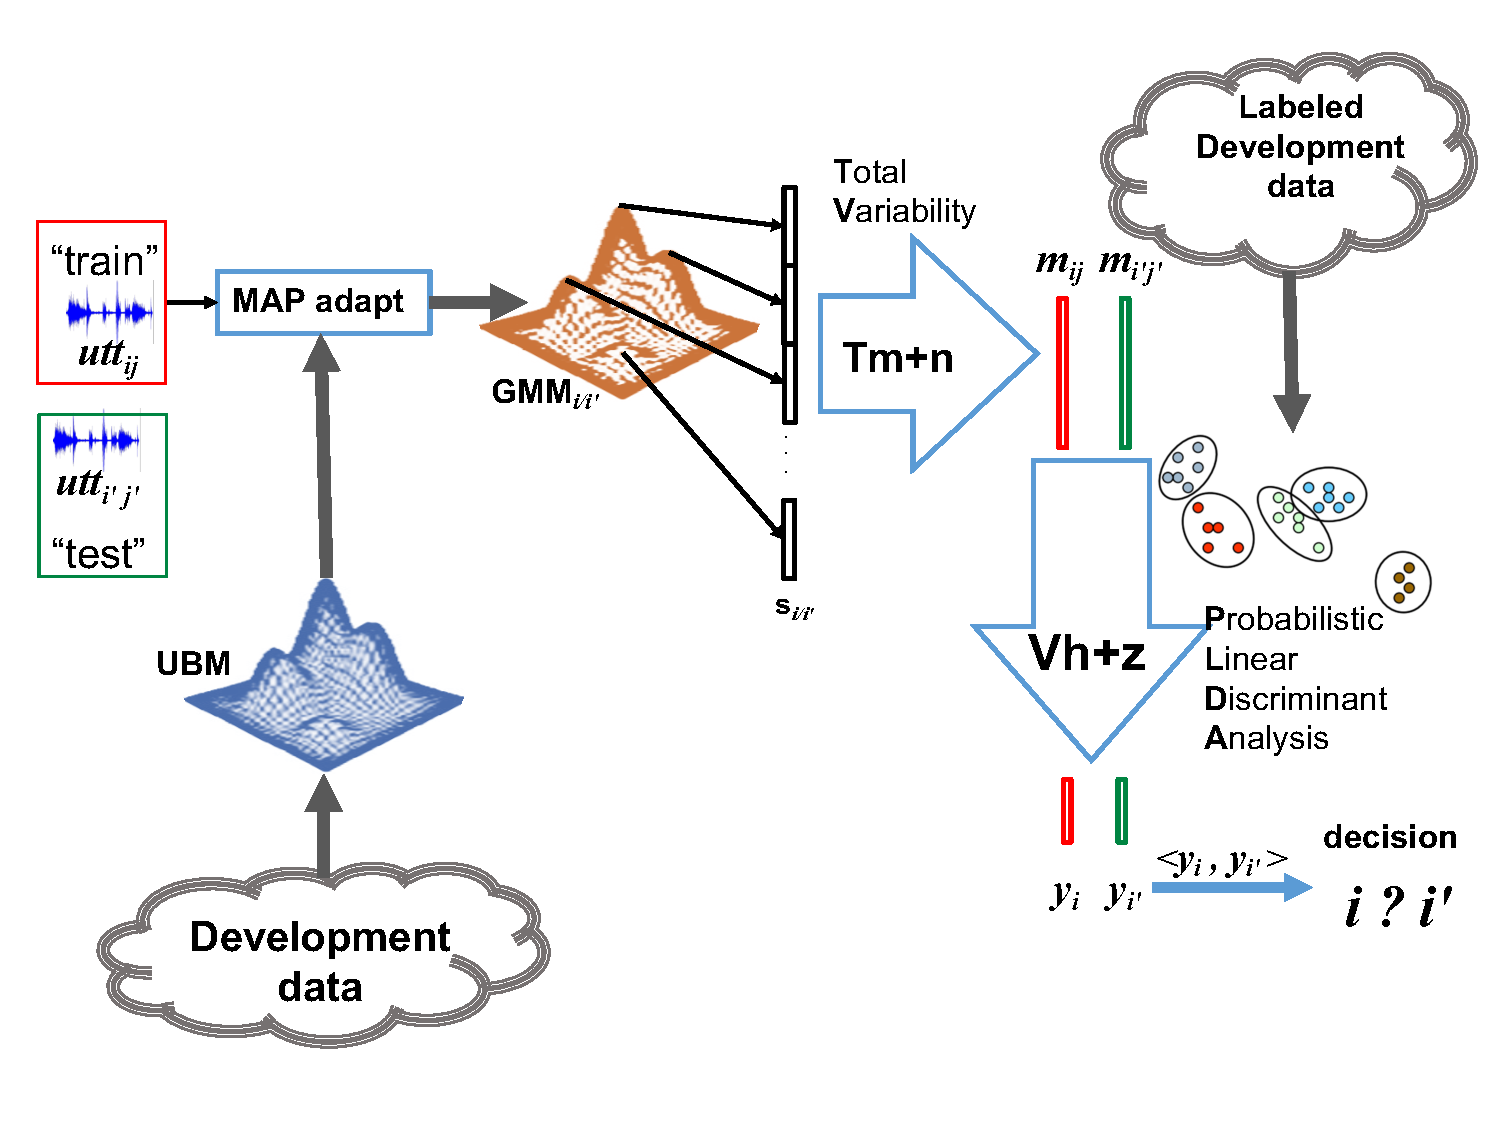
\includegraphics[height = 4in, width=0.9\textwidth]{figures/ivector_plda}
	\vspace{-3mm}
	\caption{\it Overview of i-Vector/PLDA system.}
	\label{fig:ivector_plda}
	\vspace{-3mm}
\end{figure}

The first step is extract to i-Vectors from a collection of audio files (or a single audio file), provided for each speaker. 
i-Vectors are obtained by compressing Gaussian mean super-vectors. 
Super-vectors are a concatenation of GMM means. 
Since GMMs are typically composed of 512 (or more) Gaussian mixtures, the concatenated GMM means result in incredibly large super-vectors (36-dimensional MFCC means $\times$ 512 Gaussian mixtures). 
Therefore, i-Vectors can be viewed as a dimension reduction technique to reduce the dimension of super-vectors. 
This is done through a factor analysis process that represents super-vectors as factor loadings of a Total Variability (TV) matrix. 
The factor loading weights are called i-Vectors (denoted ${\bf m}$ in Fig.~\ref{fig:ivector_plda}). 
TV matrix can be trained using unlabeled development data (typically the same data used to train the UBM). 

An i-Vector is provided for the train and test components in each trial. 
The next step is to compare these two i-Vectors to determine whether they represent the same speaker. 
Many methods have been proposed to compare i-Vectors, the most popular of which is probabilistic linear discriminant analysis (PLDA). 
PLDA has been thoroughly explained in Chapter~\ref{chapter:backend}, but it can also be viewed as a factor analysis method to remove certain (unwanted) variabilities from the i-Vectors. 
The likelihood ratio provided by PLDA is typically used to determine the certainty to which the system believes the two i-Vectors from a trial belong to the same speaker. 


\begin{thesisbib}
\bibliography{refs.bib}
\end{thesisbib}  % <-- THIS LINE IS REQUIRED!

\begin{vita}
Navid Shokouhi was born in Ahvaz, Khuzestan, Iran on June 9, 1989, to Hossein Shokouhi and Manzar Mohammadi. 
His parents decided to move to Australia soon after he was born.
%He was raised bilingual, speaking Farsi at home with his parents and English at school and with his friends. 
At the age of 9 he and his parents moved back to Ahvaz, where his father was hired as an Assistant Professor of Linguistics in Shahid Chamran University. 
Navid attended Amirkabir University of Technology (AUT) in Tehran as a Bachelors student in Electrical Engineering in 2007. 
He graduated with a Degree in Electrical Engineering in 2011. 
As a senior undergraduate student he worked with Dr. Hamid Sheikhzadeh for his final project. 
There he was introduced to basic principles of speech signal processing. 
His undergraduate senior project at AUT was on voice conversation and speech synthesis. 
In the Fall of 2011 he moved to the United States to pursue a PhD degree under the supervision of Prof. John H. L. Hansen at the University of Texas at Dallas (UTD). 
In the Center for Robust Speech Systems (CRSS) at UTD he primarily focused on speaker recognition, specifically in multi-speaker environments. 
He participated in a number of NIST Speaker Recognition Evaluations during his time as a PhD student at CRSS. 
In 2013 he was awarded the IBM best student paper award by the IEEE signal processing society alongside three other student co-authors for a paper in ICASSP 2013 on the CRSS system for speaker recognition in the 2012 NIST SRE challenge. 
In the Summer of 2015 he was recruited as an intern at ToyTalk Inc., where he developed speech processing tools for mobile platforms. 
He is expected to graduate with a PhD degree in Electrical Engineering -- Signal Processing from the University of Texas at Dallas in 2016. 
\end{vita}

\end{document}

